\documentclass[
    % -- opções da classe memoir --
    12pt,                % tamanho da fonte
    %openright,            % capítulos começam em pág ímpar (insere página vazia caso preciso)
    oneside,            % twoside para impressão em verso e anverso. Oposto a oneside
    a4paper,            % tamanho do papel.
    % -- opções da classe abntex2 --
    %section=TITLE,        % títulos de capítulos convertidos em letras maiúsculas
    %section=TITLE,        % títulos de seções convertidos em letras maiúsculas
    %subsection=TITLE,    % títulos de subseções convertidos em letras maiúsculas
    %subsubsection=TITLE,% títulos de subsubseções convertidos em letras maiúsculas
    % -- opções do pacote babel --
    english,            % idioma adicional para hifenização
    french,                % idioma adicional para hifenização
    spanish,            % idioma adicional para hifenização
    brazil                % o último idioma é o principal do documento
    ]{abntex2}

% ---
% Pacotes básicos
% ---
\usepackage{lmodern}            % Usa a fonte Latin Modern            
\usepackage[T1]{fontenc}        % Selecao de codigos de fonte.
\usepackage[utf8]{inputenc}        % Codificacao do documento (conversão automática dos acentos)
\usepackage{indentfirst}        % Indenta o primeiro parágrafo de cada seção.
\usepackage{lastpage}            % Usado pela Ficha catalográfica

\usepackage{color}                % Controle das cores
%\usepackage[demo]{graphicx}
\usepackage{graphicx}            % Inclusão de gráficos
\usepackage{microtype}             % para melhorias de justificação
\usepackage{amsmath}


\usepackage[position=bottom]{subfig}
%\usepackage[hang]{subfigure}
%\usepackage{subfigure}

%\usepackage[utf8]{inputenc}
\usepackage{algorithm}
\usepackage{algpseudocode}
%\usepackage{algorithm2e}

\makeatletter
\renewcommand{\ALG@name}{Algoritmo}
\makeatother
\renewcommand{\listalgorithmname}{Lista de Algoritmos}

\usepackage[brazil]{babel}
\usepackage[justification=centering]{caption}

%\newcommand\algorithmicprocedure{\textbf{procedure}}
%\newcommand{\algorithmicendprocedure}{\algorithmicend\ \algorithmicprocedure}
%\makeatletter
%\newcommand\PROCEDURE[3][default]{%
%  \ALC@it
%  \algorithmicprocedure\ \textsc{#2}(#3)%
%  \ALC@com{#1}%
%  \begin{ALC@prc}%
%}
%\newcommand\ENDPROCEDURE{%
%  \end{ALC@prc}%
%  \ifthenelse{\boolean{ALC@noend}}{}{%
%    \ALC@it\algorithmicendprocedure
%  }%
%}
\newenvironment{ALC@prc}{\begin{ALC@g}}{\end{ALC@g}}
\makeatother

\algnewcommand\algorithmicforeach{\textbf{for each}}
\algdef{S}[FOR]{ForEach}[1]{\algorithmicforeach\ #1\ \algorithmicdo}


% adicionado por Ting
\setlength{\marginparwidth}{2cm}
\usepackage{todonotes}
%\usepackage{soul}
\usepackage[normalem]{ulem}
\usepackage{hyperref}

%\setlength\afterchapskip{\lineskip}




% ---
        
% ---
% Pacotes adicionais, usados apenas no \^{a}mbito do Modelo Can\^{o}nico do abnteX2
% ---
\usepackage{lipsum}				% para gera\c{c}\~{a}o de dummy text
\usepackage{nomencl}
\usepackage{amsmath}
\usepackage{bbm}
\usepackage{multirow}
\usepackage{rotating}
\usepackage{pdfpages}
%\usepackage[font=footnotesize]{subfig}
\usepackage{booktabs}
\usepackage{pdflscape}
\usepackage{chngcntr}
\usepackage{amsmath,amsfonts,amssymb}

\usepackage{algorithm}

\usepackage{amsmath,amsfonts,amssymb}


%\let\printglossary\relax
%\let\theglossary\relax
%\let\endtheglossary\relax

\usepackage[nonumberlist,acronym,nomain]{glossaries} % nonnumberlist nao mostra as paginas nas quais os acronimos aparecem no texto
%\newglossary[tlg]{simbolos}{tld}{tdn}{Lista de símbolos}
% Generate the glossary
%\makeglossaries


\counterwithin{figure}{chapter}
\counterwithin{table}{chapter}
% Pacotes de citações
% ---
\usepackage[brazilian,hyperpageref]{backref}     % Paginas com as citações na bibl
\usepackage[alf]{abntex2cite}    % Citações padrão ABNT

\usepackage{unicamp}

% ---
% CONFiguraÇÕES DE PACOTES
% ---

% ---
% ConFigurações do pacote backref
% Usado sem a opção hyperpageref de backref
\renewcommand{\backrefpagesname}{Citado na(s) página(s):~}
% Texto padrão antes do número das páginas
\renewcommand{\backref}{}
% Define os textos da citação
\renewcommand*{\backrefalt}[4]{
    \ifcase #1 %
        Nenhuma citação no texto.%
    \or
        Citado na página #2.%
    \else
        Citado #1 vezes nas páginas #2.%
    \fi}%
% ---

%Redefinições de comando para pseudocódigo - Portugues
% Declaracoes em Português
%\algrenewcommand\algorithmicend{\textbf{fim}}
%\algrenewcommand\algorithmicdo{\textbf{faça}}
%\algrenewcommand\algorithmicwhile{\textbf{enqua%nto}}
%\algrenewcommand\algorithmicfor{\textbf{para}}
%\algrenewcommand\algorithmicif{\textbf{se}}
%\algrenewcommand\algorithmicthen{\textbf{então}%}
%\algrenewcommand\algorithmicelse{\textbf{senão}%}
%\algrenewcommand\algorithmicreturn{\textbf{devo%lve}}
%\algrenewcommand\algorithmicfunction{\textbf{fu%nção}}
%
%% Rearranja os finais de cada estrutura
%\algrenewtext{EndWhile}{\algorithmicend\ %\algorithmicwhile}
%\algrenewtext{EndFor}{\algorithmicend\ %\algorithmicfor}
%\algrenewtext{EndIf}{\algorithmicend\ %\algorithmicif}
%\algrenewtext{EndFunction}{\algorithmicend\ %\algorithmicfunction}
%
%% O comando For, a seguir, retorna 'para #1 -- %#2 até #3 faça'
%\algnewcommand\algorithmicto{\textbf{até}}
%\algrenewtext{For}[3]%
%{\algorithmicfor\ #1 $\gets$ #2 \algorithmicto\ %#3 \algorithmicdo}

% ---


% ---
% Informações de dados para CAPA e FOLHA DE ROSTO
% ---

%\tipotrabalho{Relatório de Qualificação de Mestrado}
% O preambulo deve conter o tipo do trabalho, o objetivo,
% o nome da instituição e a área de concentração

% ---


% ---
% Configurações de aparência do PDF final

% alterando o aspecto da cor azul
\definecolor{blue}{RGB}{41,5,195}

% informações do PDF
\makeatletter
\hypersetup{
         %pagebackref=true,
        pdftitle={\@title},
        pdfauthor={\@author},
        pdfsubject={\imprimirpreambulo},
        pdfcreator={LaTeX with abnTeX2},
        pdfkeywords={abnt}{latex}{abntex}{abntex2}{trabalho acadêmico},
        colorlinks=true,               % false: boxed links; true: colored links
        linkcolor= blue,              % color of internal links
        citecolor=blue,                % color of links to bibliography
        filecolor=magenta,              % color of file links
        urlcolor=blue,
        bookmarksdepth=4
}
\makeatother
% ---

% ---
% Espaçamentos entre linhas e parágrafos
% ---

% O tamanho do parágrafo é dado por:
\setlength{\parindent}{2cm}

% Controle do espaçamento entre um parágrafo e outro:
\setlength{\parskip}{0.2cm}  % tente também \onelineskip

\setlength\afterchapskip{\lineskip}

\titulo{Renderização Interativa de Funções de Distribuição de Orientação em Ambiente de Visualização Multimodal}
\autor{Daniel Xavier Silva}
\orientador{Profa. Dra. Wu Shin-Ting}
\local{Campinas}
\data{2021}
\instituicao{%
  UNIVERSIDADE ESTADUAL DE CAMPINAS
    \par
    Faculdade de Engenharia Elétrica e de Computação
  %Departamento de Engenharia de Computação e Automação Industrial - DCA\par
  %Faculdade de Engenharia Elétrica e de Computação - FEEC
  }
  \tipotrabalho{Dissertação (Mestrado)}
  \preambulo{Dissertação apresentada à Faculdade de Engenharia Elétrica e de Computação da Universidade Estadual de Campinas como parte dos requisitos exigidos para a obtenção do título de Mestre em Engenharia Elétrica, na Área de Engenharia de Computação.}

% ---
% compila o indice
% ---
\makeindex
% ---

% ----
% Início do documento
% ----

\begin{document}



% ----------------------------------------------------------
% ELEMENTOS PRÉ-TEXTUAIS
% ----------------------------------------------------------
% \pretextual

% ---
% Capa
% ---
% ---

\imprimircapa
% ---
% Folha de rosto
% (o * indica que haverá a ficha bibliográfica)
% ---
\imprimirfolhaderosto*
% ---

% ---
% Inserir a ficha bibliografica
% ---
\begin{fichacatalografica}
    \vspace*{\fill}
    \begin{center}
        \textsc{Inclua aqui o pdf com a ficha catalogr\'{a}fica fornecida pela BAE.}
    \end{center}
    \vspace*{\fill}
    %\includepdf{fig_ficha_catalografica.pdf}
\end{fichacatalografica}

% Isto é um exemplo de Ficha Catalográfica, ou ``Dados internacionais de
% catalogação-na-publicação''. Você pode utilizar este modelo como referência.
% Porém, provavelmente a biblioteca da sua universidade lhe fornecerá um PDF
% com a ficha catalográfica definitiva após a defesa do trabalho. Quando estiver
% com o documento, salve-o como PDF no diretório do seu projeto e substitua todo
% o conteúdo de implementação deste arquivo pelo comando abaixo:
%
% \begin{fichacatalografica}
%     \includepdf{fig_ficha_catalografica.pdf}
% \end{fichacatalografica}
% \begin{fichacatalografica}
%     \vspace*{\fill}                    % Posição vertical
%     \hrule                            % Linha horizontal
%     \begin{center}                    % Minipage Centralizado
%     \begin{minipage}[c]{12.5cm}        % Largura
    
%     \imprimirautor
    
%     \hspace{0.5cm} \imprimirtitulo  / \imprimirautor. --
%     \imprimirlocal, \imprimirdata-
    
%     \hspace{0.5cm} \pageref{LastPage} p. : il. (algumas color.) ; 30 cm.\\
    
%     \hspace{0.5cm} \imprimirorientadorRotulo~\imprimirorientador\\
    
%     \hspace{0.5cm}
%     \parbox[t]{\textwidth}{\imprimirtipotrabalho~--~\imprimirinstituicao,
%     \imprimirdata.}\\
    
%     \hspace{0.5cm}
%         1. Palavra-chave1.
%         2. Palavra-chave2.
%         I. Orientador.
%         II. Universidade xxx.
%         III. Faculdade de xxx.
%         IV. Título\\             
    
%     \hspace{8.75cm} CDU 02:141:005.7\\
    
%     \end{minipage}
%     \end{center}
%     \hrule
% \end{fichacatalografica}


% \includepdf{folhadeaprovacao_final.pdf}
%
% --- Inserir folha de aprova\c{c}\~{a}o ---

% Isto \'{e} um exemplo de Folha de aprova\c{c}\~{a}o, elemento obrigat\'{o}rio da NBR
% 14724/2011 (se\c{c}\~{a}o 4.2.1.3). Voc\^{e} pode utilizar este modelo at\'{e} a aprova\c{c}\~{a}o
% do trabalho. Ap\'{o}s isso, substitua todo o conte\'{u}do deste arquivo por uma
% imagem da p\'{a}gina assinada pela banca com o comando abaixo:
%
% \begin{folhadeaprovacao}
% \includepdf{folhadeaprovacao_final.pdf}
% \end{folhadeaprovacao}
%
\begin{folhadeaprovacao}

  \begin{center}
    COMISS\~{A}O JULGADORA - TESE DE DOUTORADO
    %\textsc{Inclua aqui a folha de assinaturas.}
\end{center}
\noindent
\begin{minipage}{\textwidth}\SingleSpacing
Candidato(a): Daniel Xavier Silva     RA: 229988

Data de defesa: XX de MES de 202X

T\'{i}tulo da Tese: "XXXXXXXXXXXXXXXXXXXXXXXXXXXXXXX"
\vspace{2cm}

Profa. Dra. Xxxxxxxxxx (Presidente)

Profa. Dra. xxxxxxx

Profa. Dra. xxxxxxx

Profa. Dra. xxxxxxxxx

Profa. Dra xxxxxxxxxxxx

\vspace{2cm}

A Ata de Defesa, com as respectivas assinaturas dos membros da Comissão Julgadora, encontra-se no SIGA (Sistema de Fluxo de Dissertação/Tese) e na Secretaria de Pós-Graduação da Faculdade de Engenharia Elétrica e de Computação.
\end{minipage}

\end{folhadeaprovacao}
% ---

% ---
% Dedicatória
% ---
\begin{dedicatoria}
   \vspace*{\fill}
   \centering
   \noindent
   \textit{!!Eu dedico este trabalho} \vspace*{\fill}
\end{dedicatoria}
% ---

% ---
% Agradecimentos
% ---
% ---
\begin{agradecimentos}
    !!O presente trabalho foi realizado com apoio do CNPq, Conselho Nacional de Desenvolvimento Científico  e Tecnológico – Brasil.
\end{agradecimentos}

% ---
% Epígrafe
% ---
\begin{epigrafe}
    \vspace*{\fill}
	\begin{flushright}
		\textit{``Escreva aqui a sua ep\'{\i}grafe (Opcional)''\\
		(Cita\c{c}\~{a}o)}
	\end{flushright}
\end{epigrafe}
% ---

% ---
% RESUMOS

%% resumo em português
\setlength{\absparsep}{18pt} % ajusta o espaçamento %dos parágrafos do resumo
\begin{resumo}

A ressonância magnética ponderada por difusão (DWI) é uma modalidade de imageamento que mensura a difusão de fluidos. Aplicada ao cérebro, o DWI é único no que diz respeito à quantificação deste fenômeno na água em tecido vivo. Na substância branca do cérebro, a difusão tem a mesma direção preferencial de suas fibras, o que possibilita a inferência da sua arquitetura \textit{in-vivo} e de forma não-invasiva. Para este fim, há métodos de imageamento que modelam este fenômeno, sendo o imageamento por tensor de difusão (\textit{Diffusion Tensor Imaging}, DTI) o mais conhecido e difundido clinicamente. A partir do tensor, métricas, como informações referentes à direção preferencial de difusão, possibilitam o inferimento da arquitetura da substância branca e tornam viável estudos e diagnósticos. No entanto, o modelo utilizado no DTI falha no mapeamento do comportamento difusão em regiões de substância branca onde há duas ou mais populações de fibras localizadas no mesmo \textit{voxel}. Face a este problema, grupos de pesquisa passaram a propor métodos de mais alta ordem para modelar a difusão com o objetivo de superar o problema do DTI e possibilitar o inferimento da arquitetura da substância branca de forma mais precisa. Este trabalho tem como objetivo a integração de um método de alta ordem em um ambiente de visualização multimodal interativo para processamento de volumes de difusão, e sua visualização interativa em glifos. Apresentamos uma introdução aos métodos de alta ordem e sua motivação e detalhamos a implementação computacional do método Amostragem Generalizado no Espaço-Q (\textit{Generalized Q-Space Imaging}, GQI). Afim de proporcionar uma visão tridimensional dos dados obtidos através do método, desenvolvemos um algoritmo interativo acelerado por GPU que mapeiam os dados provenientes de métodos de alta ordem em glifos. Os glifos propiciam a inferência da trajetória de fibras subjacentes e avaliação dos dados gerados, que é fundamental para pesquisa na área.


\vspace{\onelineskip}
\noindent\textbf{Palavras-chave}: imageamento generalizado no espaço-Q, HARDI, ressonância magnética ponderada por difusão, renderização de glifos, computação gráfica, plotagem polar esférica
\end{resumo}
\pagebreak
%
%% resumo em inglês
\begin{resumo}[Abstract]
 \begin{otherlanguage*}{english}
 
Diffusion-weighted magnetic resonance (DWI) is an imaging modality that measures fluid diffusion. Applied to the brain, DWI is unique when it comes to quantifying this phenomenon in water in living tissue. In the white matter of the brain, the diffusion has the preferential direction of its fibers, which allows the inference of its \textit{in-vivo} architecture and noninvasively. For this purpose, there are imaging methods that model this phenomenon, and the diffusion tensor imaging (DTI) is the most well-known and clinically disseminated. From the tensor metrics, such as information regarding the preferred direction of diffusion, it is possible to infer the white matter architecture and make studies and diagnoses viable. However, the model used in DTI cannot resolve regions of white matter where there are two or more fiber populations in the same voxel. Facing this problem, research groups started to propose higher-order methods to model a diffusion in order to overcome the DTI problem and make it possible to infer the white matter architecture more precisely. This work aims to integrate a high-order method in an interactive multimodal visualization environment for processing diffusion volumes, and its interactive visualization in glyphs. We present an introduction to high-order methods and their motivation and detail the computational implementation of the Generalized Q-Sampling Imaging. In order to provide a three-dimensional view of the data obtained through the method, we developed an interactive GPU-accelerated algorithm that maps the data from the high-order method into glyphs. The glyphs provides the inference of the underlying fiber trajectory and evaluation of the generated data, which have great utility for the research in the area.

\vspace{\onelineskip}
\noindent\textbf{Palavras-chave}: Generalized Q-Sampling Imaging, HARDI, diffusion-weighted magnetic resonance imaging, glyph rendering, computer graphics, spherical polar plot
 \end{otherlanguage*}
\end{resumo}


% ---
% inserir lista de ilustrações
% ---
\pdfbookmark[0]{\listfigurename}{lof}
\listoffigures*
\cleardoublepage
% ---

% ---
% inserir lista de tabelas
% ---
\pdfbookmark[0]{\listtablename}{lot}
\listoftables*
\cleardoublepage
% ---

% ---
% inserir lista de abreviaturas e siglas
% ---
\begin{siglas}
\item[DWI] \textit{Diffusion Weighted Magnetic Resonance Imaging} (Ressonância Magnética Ponderada por Gradientes de Difusão)
  
\item[DTI] \textit{Diffusion Tensor Imaging} (Imageamento por Tensor de Difusão)

\item[HARDI] \textit{High Angular Resolution Diffusion Imaging} (Imageamento de difusão por alta resolução angular)

%\item[FA] \textit{Fractional Anisotropy} (Anisotropia Fracionada)

%\item[QBI] \textit{Q-Ball Imaging}

\item[MRI] Magnetic Resonance Imaging (Imageamento por Ressonância Magnética)

%\item[CST] \textit{Corticospinal Tract} (Trato Corticoespinhal)

\item[GQI] \textit{Generalized Q-Sampling Imaging} (amostragem generalizada no espaço Q)

%\item[ROI] \textit{Region of Interest} (Região de Interesse)

\item[ODF] \textit{Orientation Distribution Function} (Função de Distribuição de orientação)

\item[fODF] \textit{Fiber Orientation Distribution Function} (Função de Distribuição de Orientação de Fibra)

\item[dODF] \textit{Diffusion Orientation Distribution Function} (Função de Distribuição de Orientação de Difusão)

%\item[ISMRM]    \textit{International Society for Magnetic Resonance in Medicine} (Sociedade Internacional para Ressonância Magnética em Medicina)

\item[UNICAMP] Universidade Estadual de Campinas

%\item[SLF] \textit{Superior Longitudinal Fasciculus} (Fascículo Longitudinal Superior)

%\item[CC] Corpo Caloso

%\item[GFA] \textit{Generalized Fractional Anisotropy} Anisotropia Fracionada Generalizada

\item[DSI] \textit{Diffusion Spectrum Imaging} (Imagemento por Espectro de difusão)

\item [CPU] \textit{Computer Processing Unit} (Unidade de Processamento Computacional)

\item [GPU] \textit{Graphics Processing Unit} (Unidade de Processamento Gráfico)
\end{siglas}


% ---

% ---
% inserir lista de símbolos
% ---

% ---

% ---
% inserir o sumario
% ---
\pdfbookmark[0]{\contentsname}{toc}
\tableofcontents*
\cleardoublepage
% ---



% ----------------------------------------------------------
% ELEMENTOS TEXTUAIS
% ----------------------------------------------------------
\textual



\chapter{Introdução}
\label{sec:introducao}

A difusão molecular é um processo físico que se refere ao movimento aleatório de moléculas de fluídos que resultam da sua energia térmica \cite{lebihan2006}. 
Pode-se categorizar o movimento de difusão em relação ao meio da sua ocorrência em difusão isotrópica e anisotrópica. A difusão isotrópica é quando a difusão é igual em todas as direções. Ela ocorre em um meio que não oferece obstáculos (Fig. \ref{fig::intro_difusao_isotropica}). Enquanto na difusão anisotrópica, o meio apresenta restrições ao movimento (Fig. \ref{fig::intro_difusao_anisotropica}).

No cérebro, o processo de difusão ocorre majoritariamente com moléculas de água e difere significantemente da difusão isotrópica \cite{lebihan2006}. As moléculas interagem com os corpos celulares de neurônios (substância cinzenta) e feixes de dendritos e axônios (substância branca).
Há diferenças na forma de ocorrência da difusão nas substâncias branca e cinzenta do cérebro. Na substância cinzenta, a característica da difusão é altamente complexa devido à sua organização em camadas, o que torna a interpretação do fenômeno bem desafiadora. A substância branca, por sua vez, é composta por fibras organizadas em um conjunto coerente e compactado que faz a conexão entre neurônios localizados em diferentes partes do cérebro, o que faz a difusão ter um comportamento proeminente ao longo da direção do feixe de fibras \cite{DTI_Handbook}.

A ocorrência da difusão na direção dos feixes se deve aos obstáculos impostos pelas fibras, no qual permite que a água na região entre fibras se difunda predominantemente na direção do feixe, e encontre menos obstáculos em comparação a direções mais próximas das direções perpendiculares às fibras. As barreiras ilustradas em Fig. \ref{fig::intro_difusao_anisotropica} são análogas 
às barreiras impostas pela substância branca sobre a água no cérebro.


\begin{figure}[ht]
\centering
\captionsetup[subfloat]{farskip=0pt,nearskip=0pt}
    \subfloat[Tempo = 0]{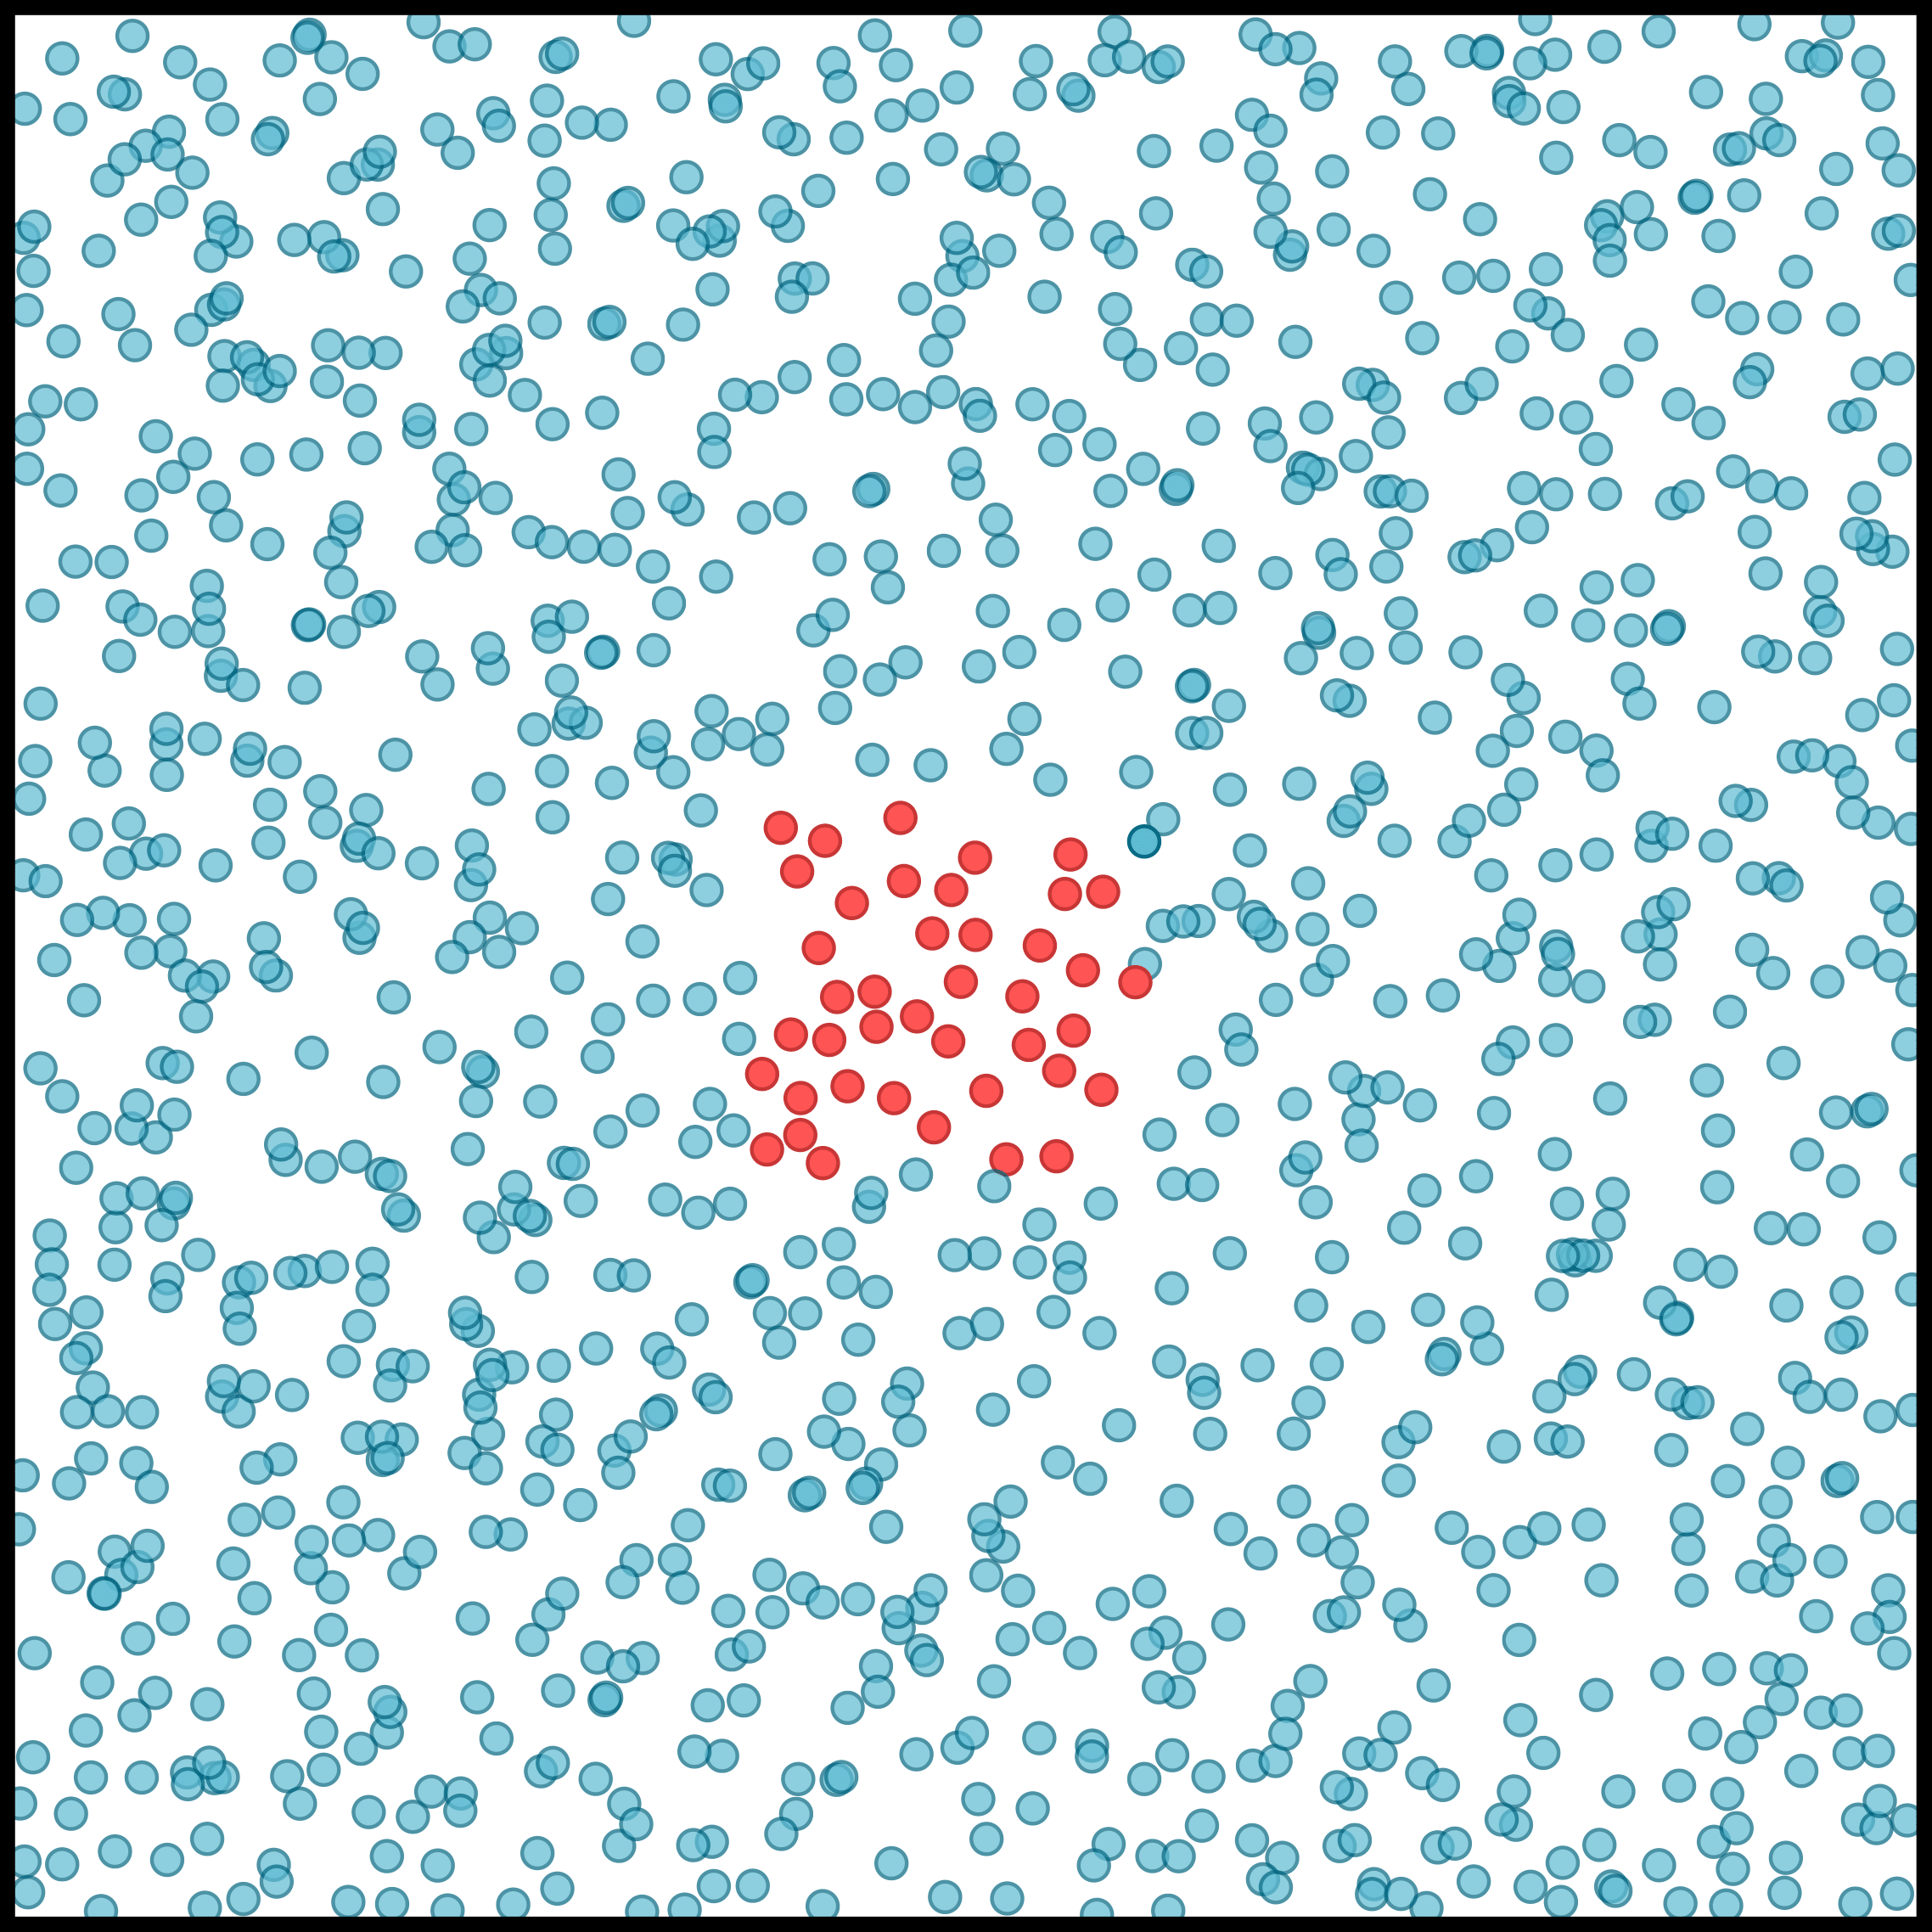
\includegraphics[width=.25\linewidth, angle=0]{figs/Introducao/Difusao_isotropica/water_molecule_t0.png}
    \label{fig::intro_difusao_isotropica_0}
    }
    \subfloat[Tempo = t]{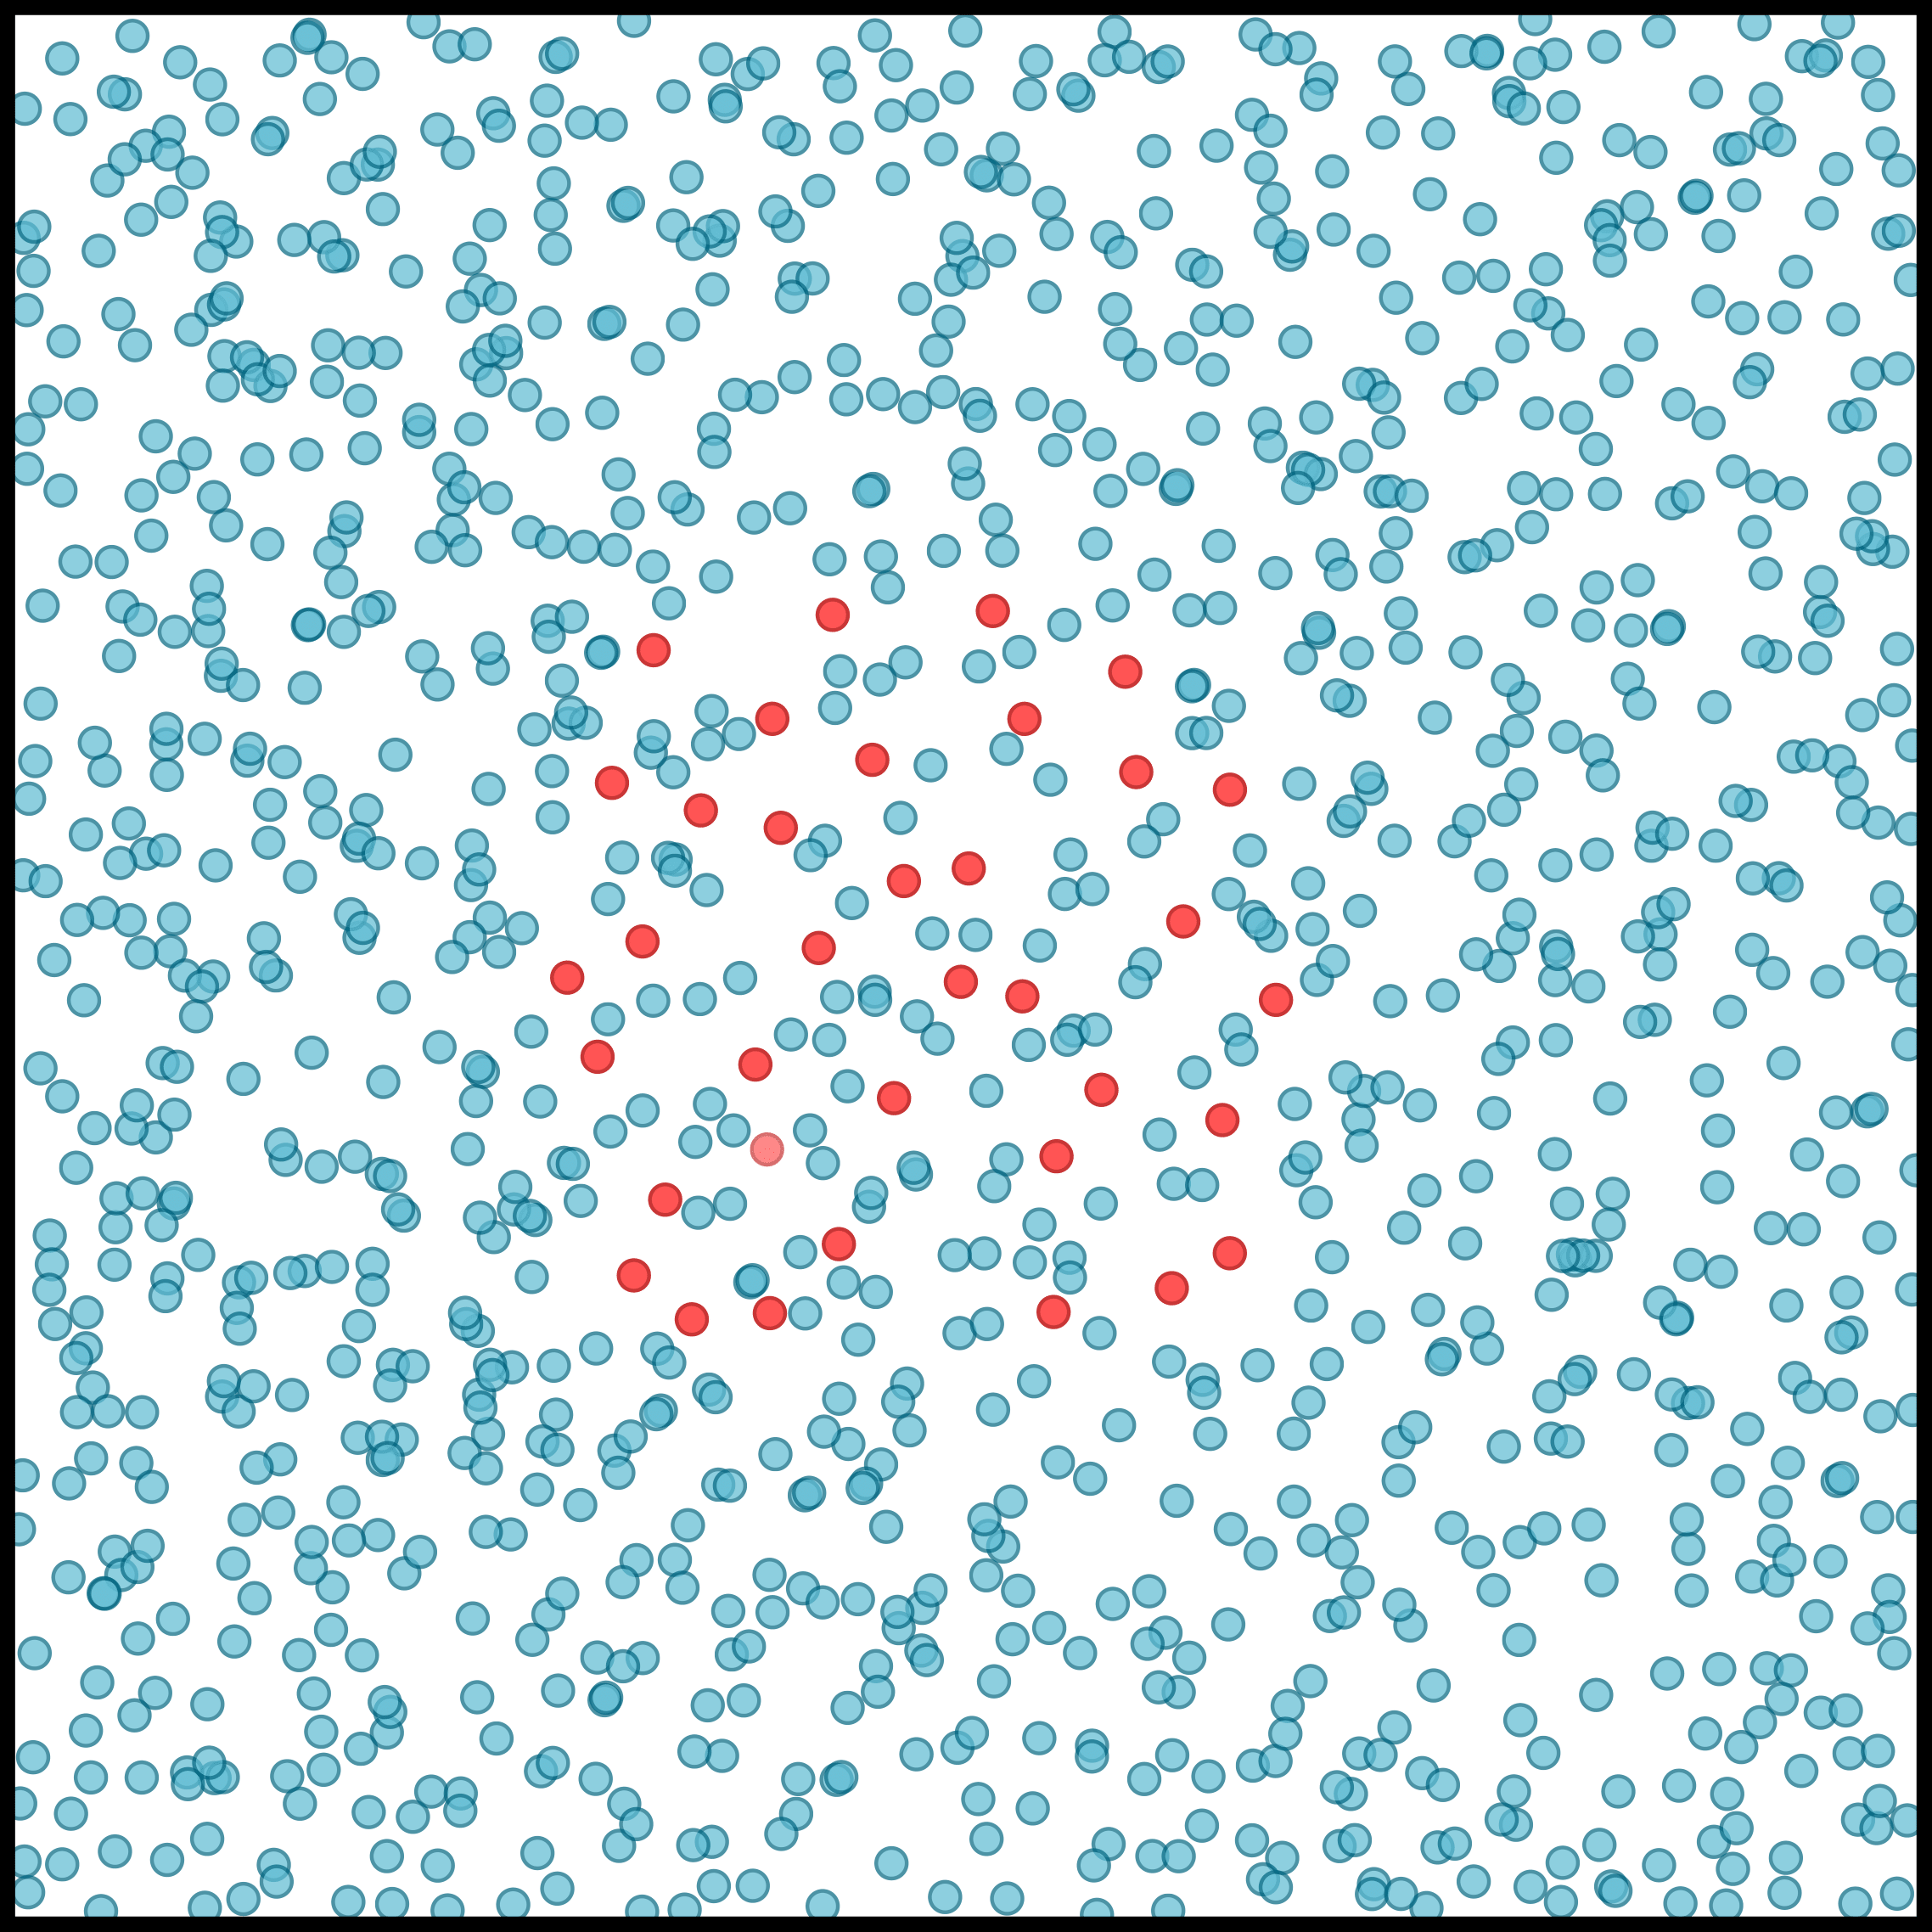
\includegraphics[width=.25\linewidth, angle=0]{figs/Introducao/Difusao_isotropica/water_molecule_t1.png}
    \label{fig::intro_difusao_isotropica_1}
    }
    \subfloat[Tempo = 2t]{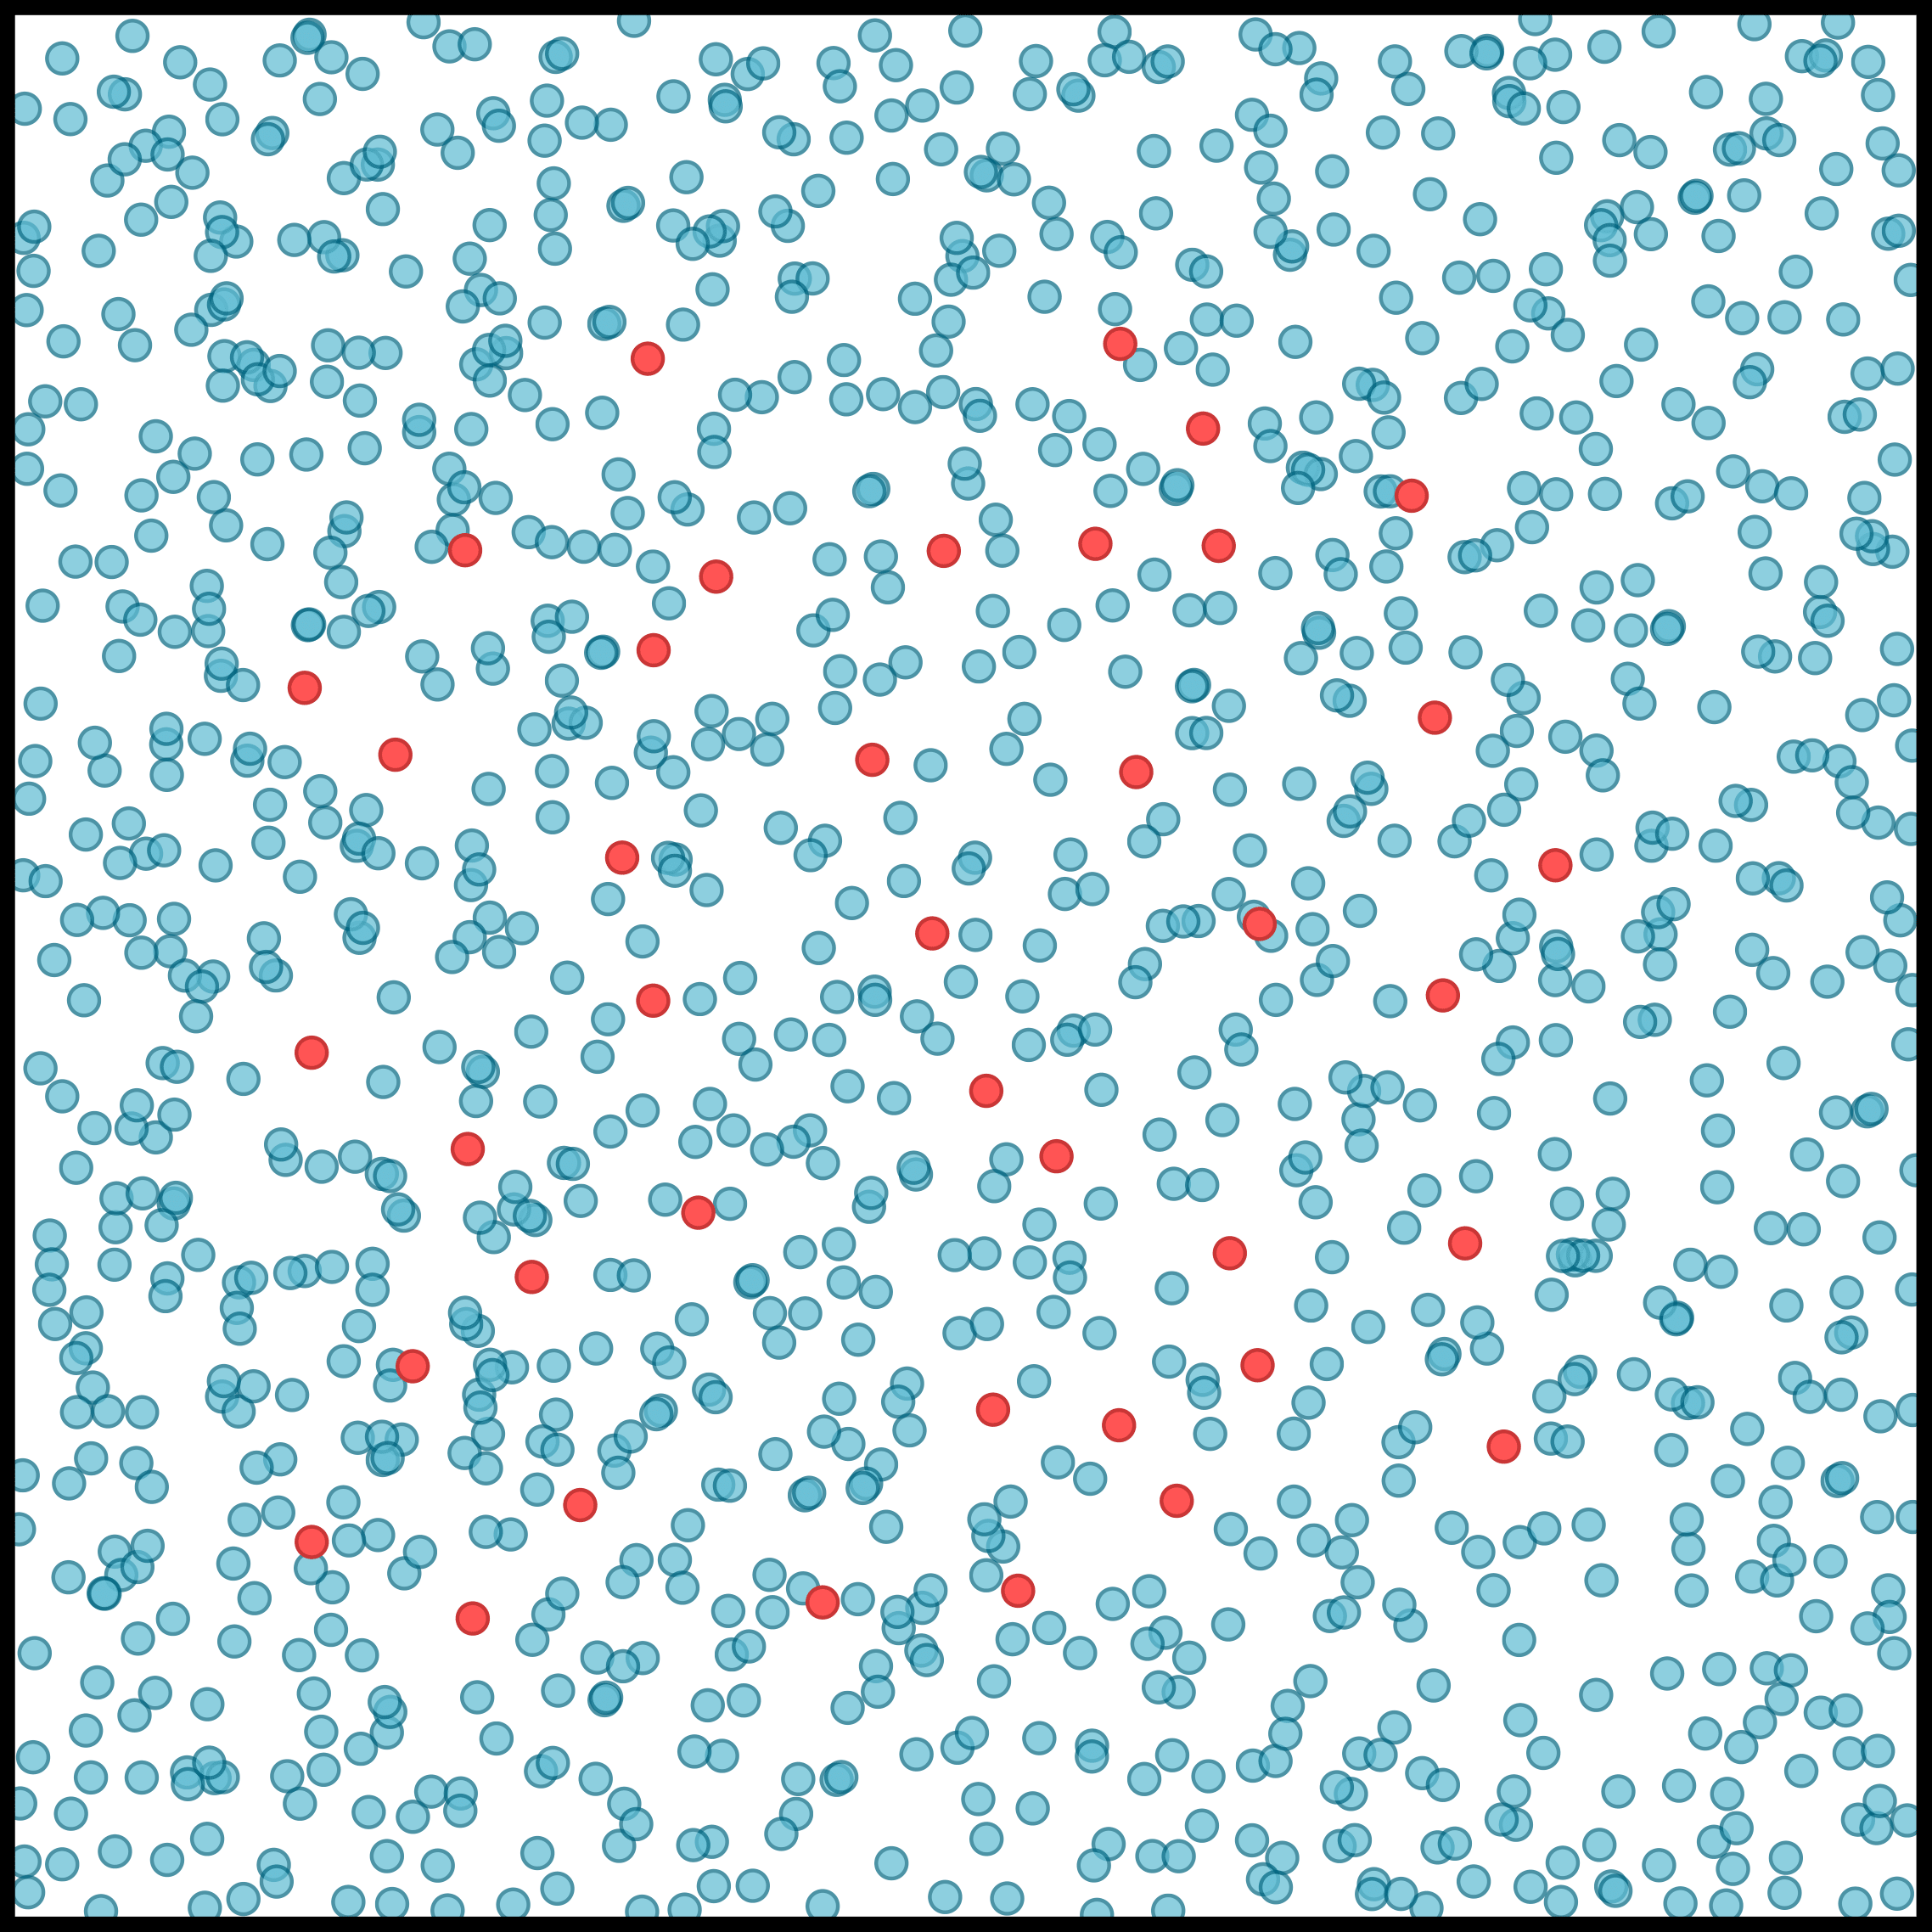
\includegraphics[width=.25\linewidth, angle=0]{figs/Introducao/Difusao_isotropica/water_molecule_t2.png}
    \label{fig::intro_difusao_isotropica_2}
    }
    \caption{Ilustração visual da difusão isotrópica. Os pontos azuis e vermelhos representam moléculas de fluidos. As moléculas em vermelho, inicialmente concentradas, se movimentam sem uma direção preferencial. \\ Fonte: \cite{voltoline2016}}
    \label{fig::intro_difusao_isotropica}
\end{figure}

\begin{figure}[ht]
\centering
\captionsetup[subfloat]{farskip=0pt,nearskip=0pt}
    \subfloat[Tempo = 0]{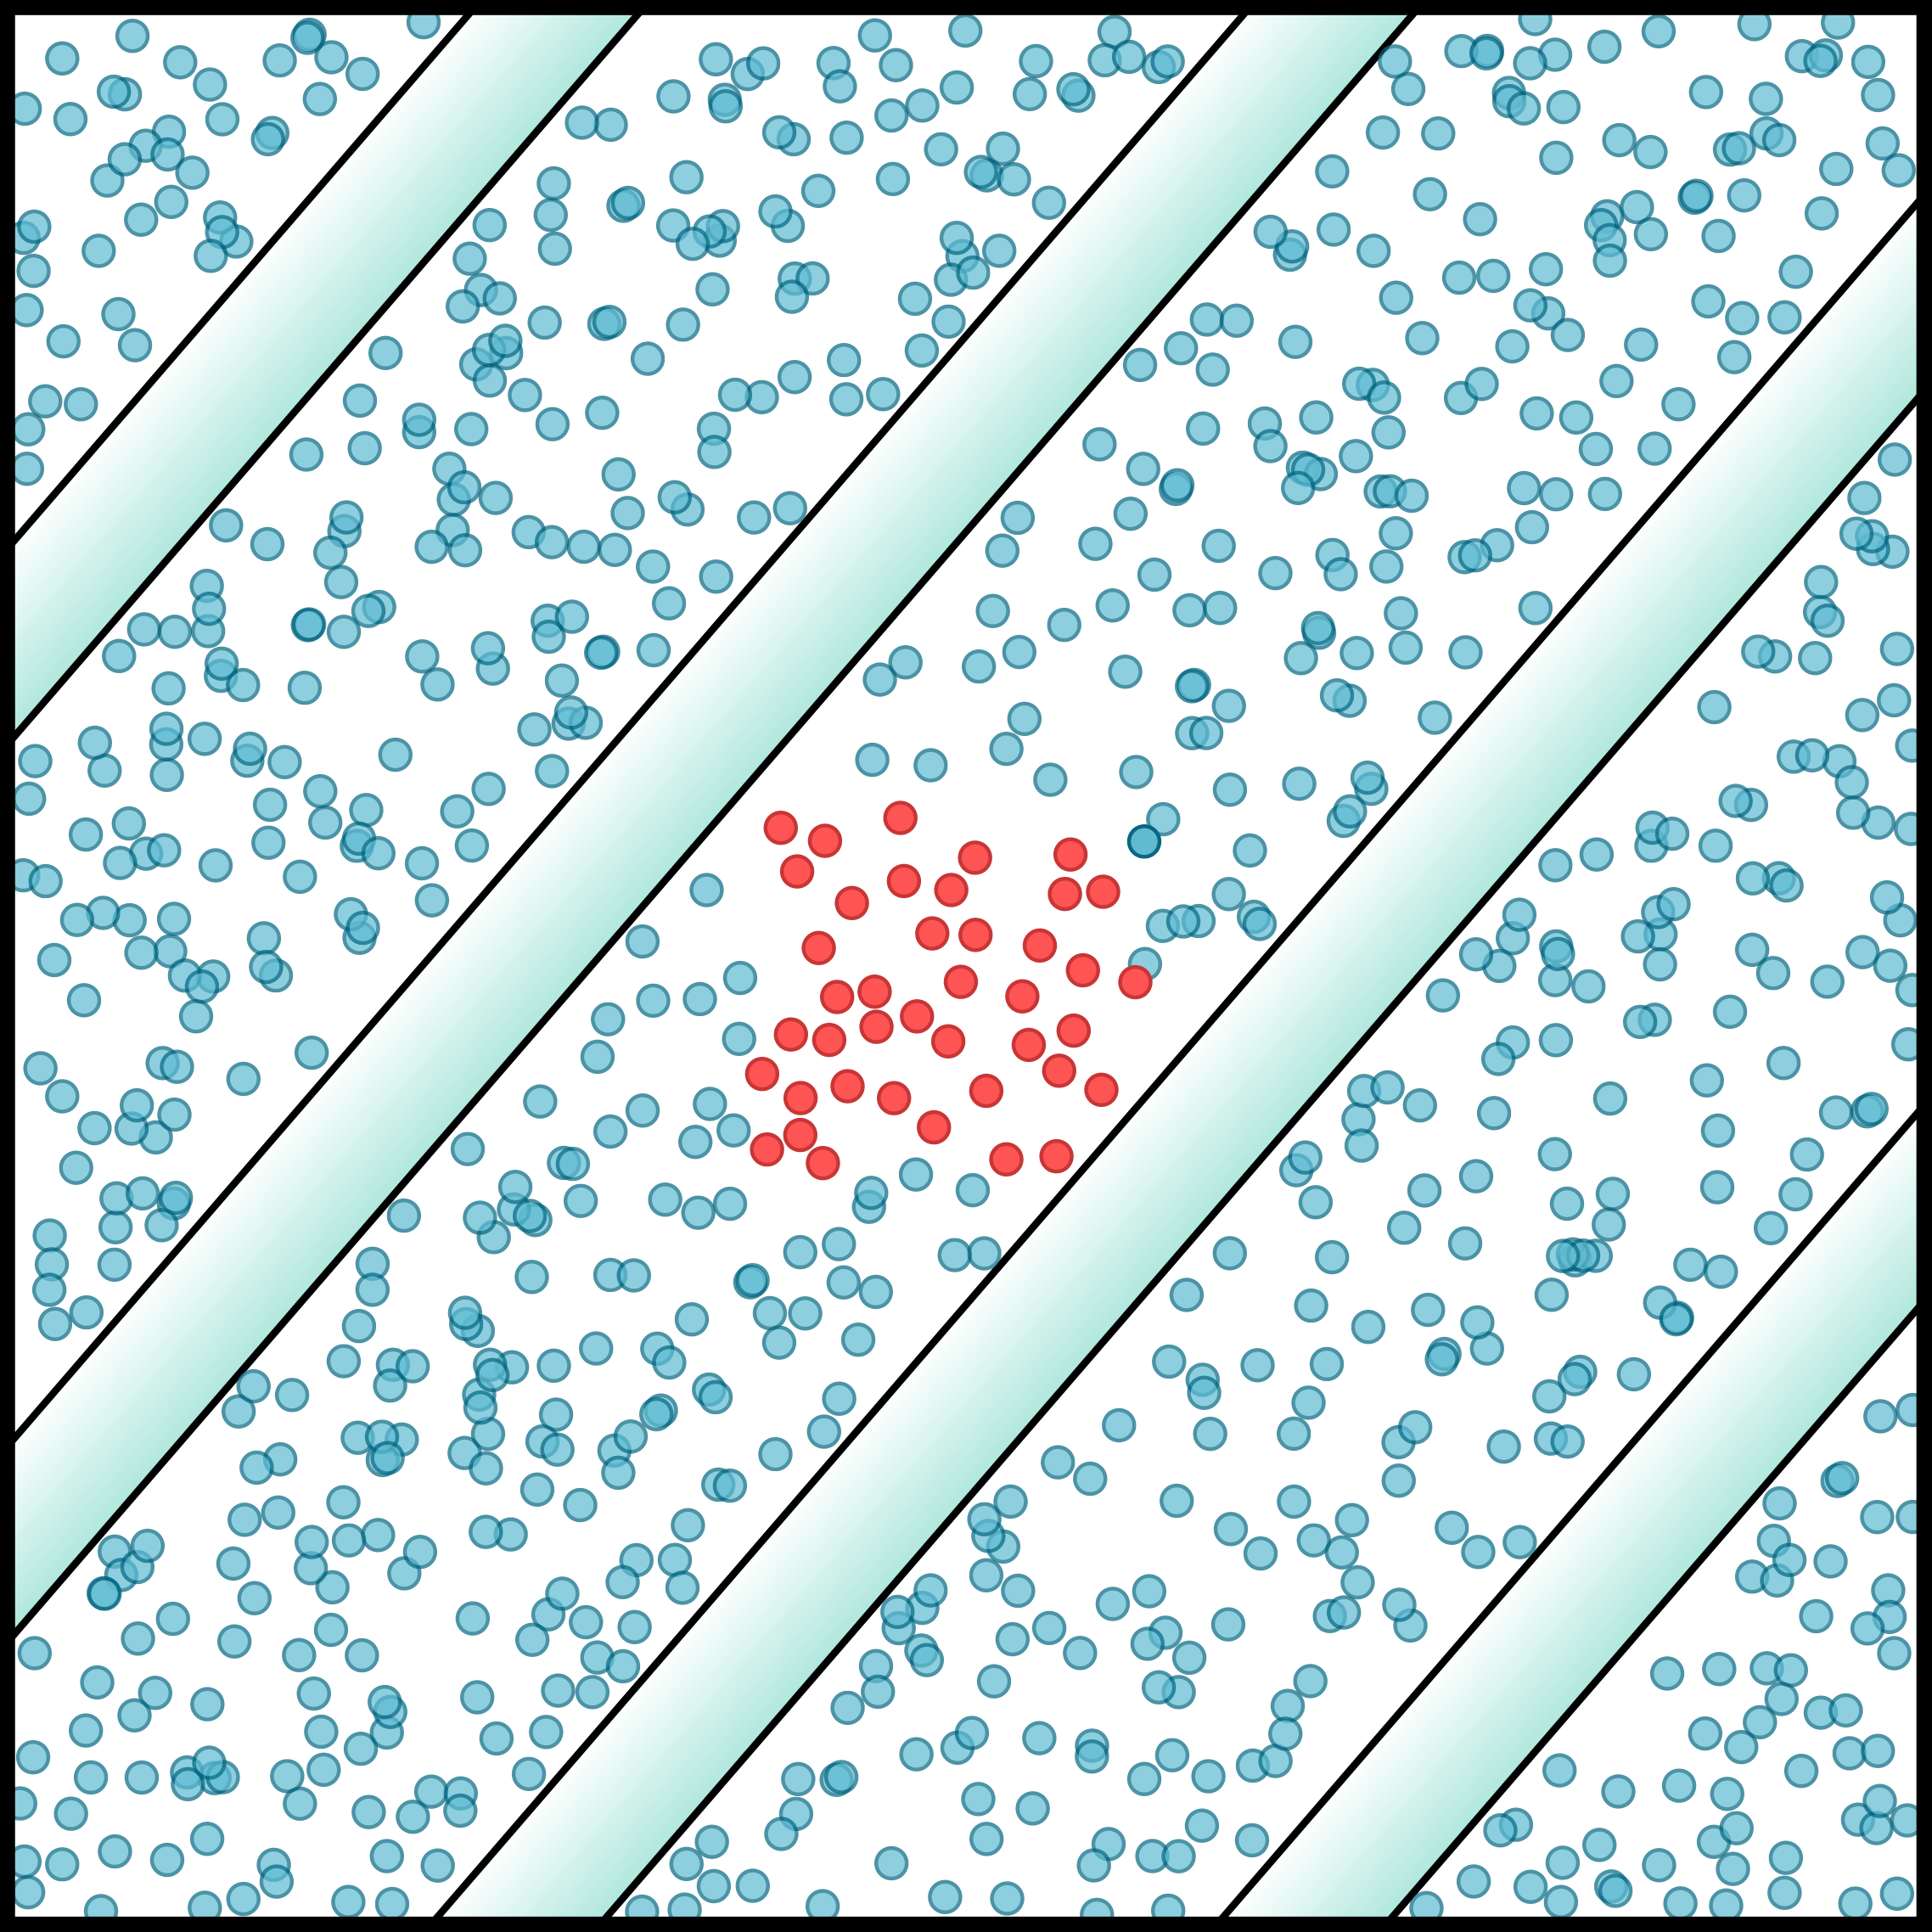
\includegraphics[width=.25\linewidth, angle=0]{figs/Introducao/Difusao_anisotropica/water_molecule_anisotropic_t0.png}
    \label{fig::intro_difusao_anisotropica_0}
    }
    \subfloat[Tempo = t]{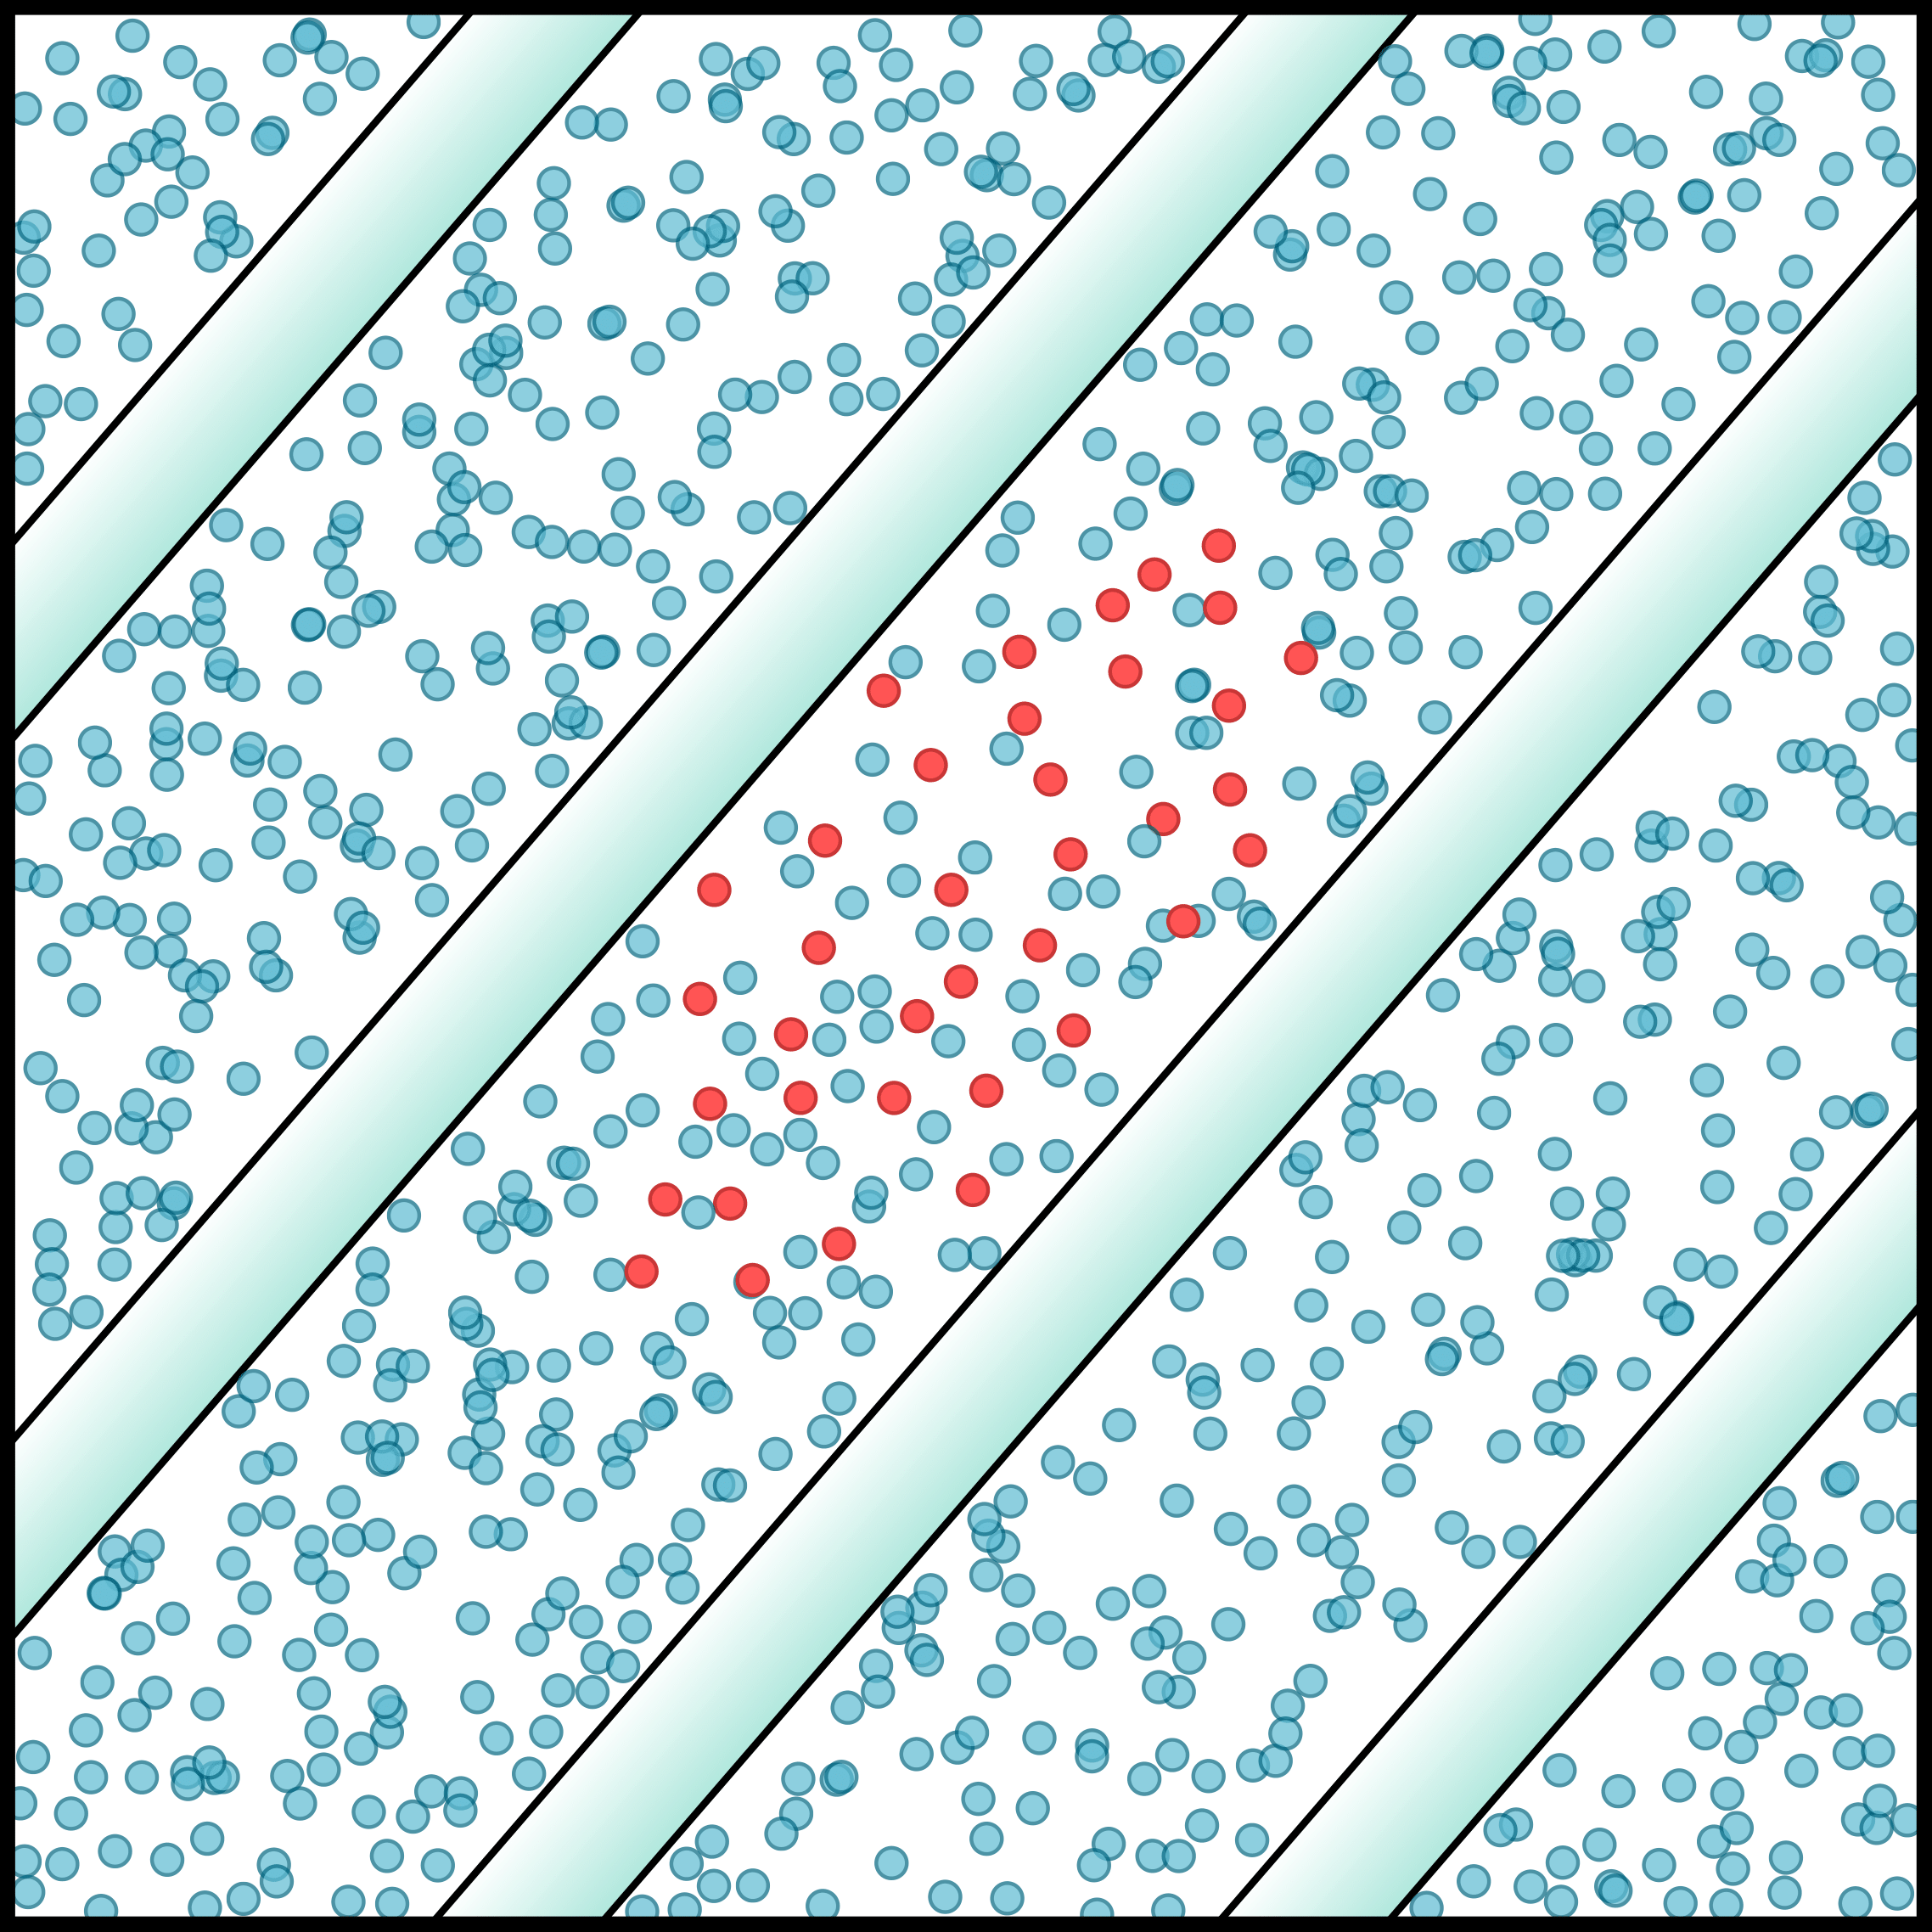
\includegraphics[width=.25\linewidth, angle=0]{figs/Introducao/Difusao_anisotropica/water_molecule_anisotropic_t1.png}
    \label{fig::intro_difusao_anisotropica_1}
    }
    \subfloat[Tempo = 2t]{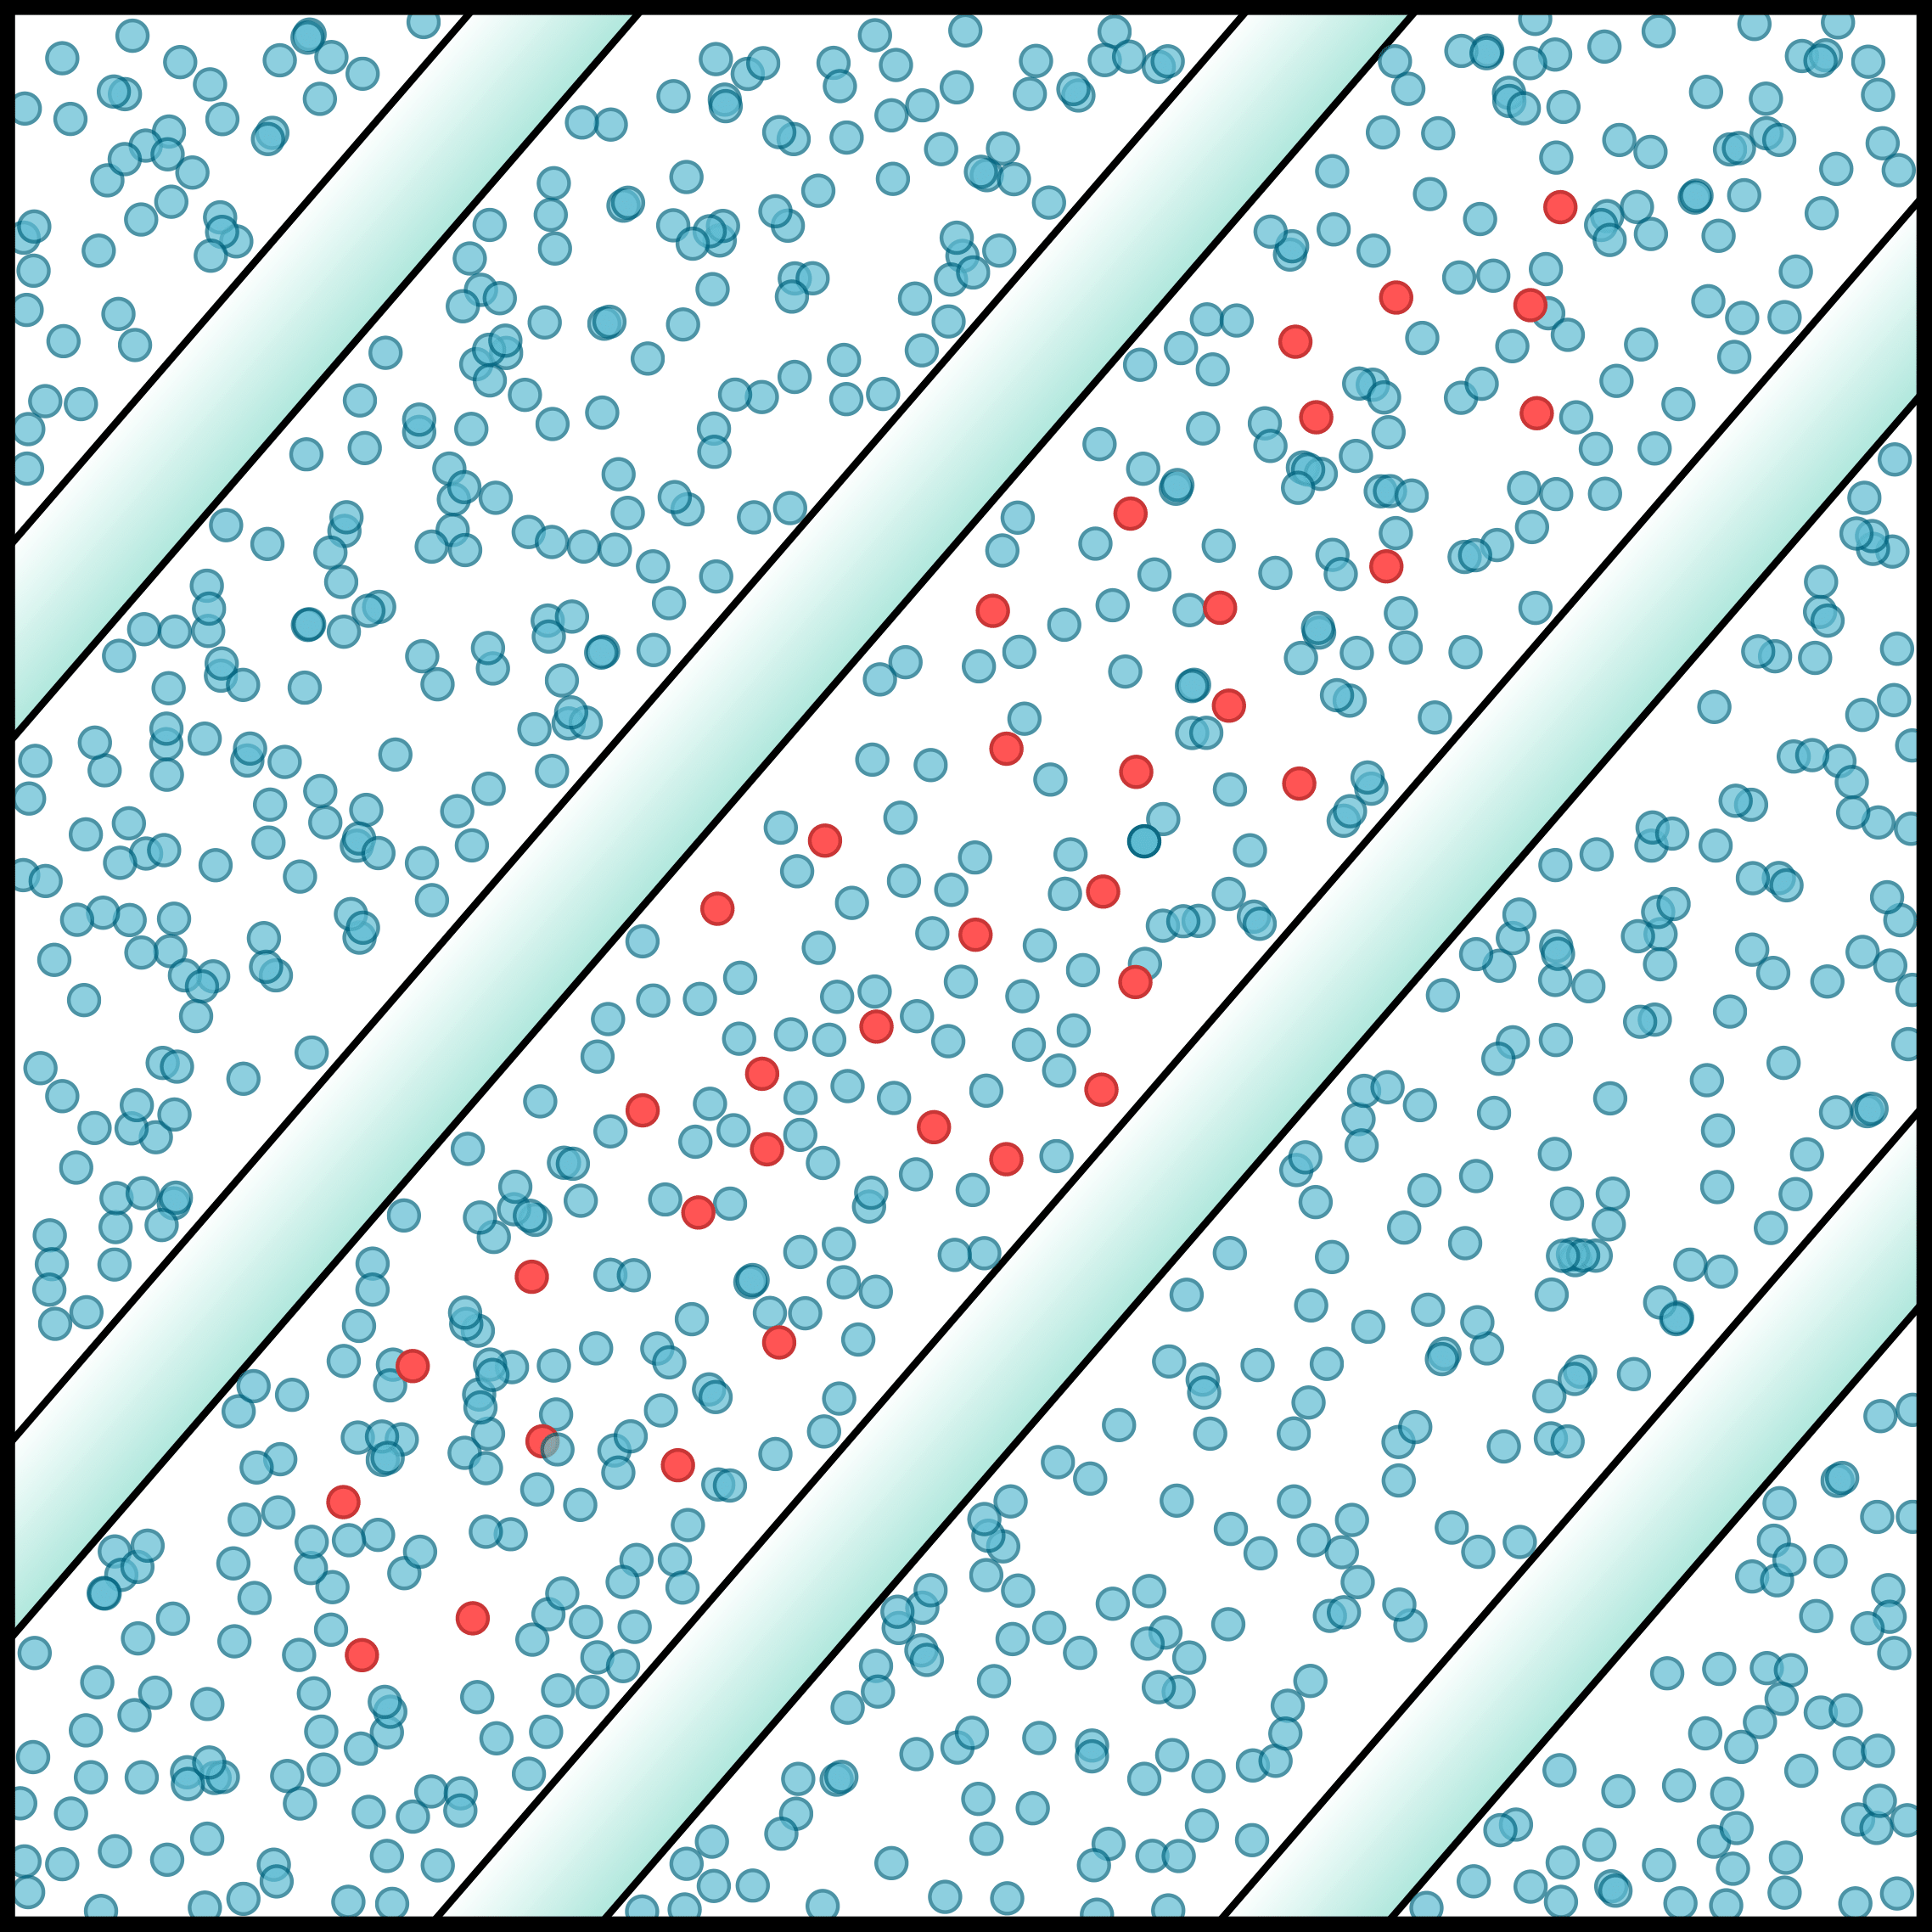
\includegraphics[width=.25\linewidth, angle=0]{figs/Introducao/Difusao_anisotropica/water_molecule_anisotropic_t2.png}
    \label{fig::intro_difusao_anisotropica_2}
    }
    \caption{Ilustração visual da difusão anisotrópica. Os pontos azuis e vermelhos representam moléculas de fluidos. As moléculas em vermelho, inicialmente concentradas, se movimentam de forma predominante em uma direção devido às restrições físicas em seu entorno. \\ Fonte: \cite{voltoline2016}
    }
    \label{fig::intro_difusao_anisotropica}
\end{figure}



%\todo{Por quê}
A medição das características de difusão da água no cérebro pode fornecer informações sobre a substância branca quanto à direção de fibras e conectividade do cérebro. Esta medição é possível através da ressonância magnética ponderada por difusão (\textit{diffusion-weighted magnetic resonance imaging} - DW-MRI ou DWI), que é no estado-da-arte o único meio não-invasivo a permitir tal informação. O DWI mede sinais de movimento browniano das moléculas de água dentro das amostras de um cérebro submetido a diferentes campos magnéticos.



%O DWI é uma forma de ressonância magnética que gera contraste a partir da difusão das moléculas de água em determinadas direções \cite{DTI_Handbook}. %A partir do sinal adquirido, há ferramentas que  possibilitam o seu mapeamento em  fibras nervosas do cérebro humano \textit{in-vivo}.

%A ressonância magnética ponderada na sequência de difusão (\textit{diffusion-weighted magnetic resonance imaging} - DW-MRI ou DWI) é uma sequência de ressonância magnética que mensura a difusão das moléculas de água em determinadas direções \cite{DTI_Handbook}. A partir do sinal adquirido, há ferramentas que  possibilitam o seu mapeamento em  fibras nervosas do cérebro humano \textit{in-vivo}.

%!!A forma mais comum para gerar o DWI é através da sequência e pulsos PGSE (\textit{Pulsed Gradient Spin Echo}).


%Na aquisição do DWI, é escaneado um conjunto de volumes em que cada um possui a ponderação de único gradiente de difusão associado a um valor-b\footnote{O valor-b é uma métrica de sensitividade para difusão e é função de parâmetros da aquisição do DWI, como função da intensidade, duração e o intervalo de tempo dos gradientes de ponderação de difusão. Quanto maior o seu valor, maior o decaimento do sinal relativo à difusão.}, e, adicionalmente, um ou mais volumes sem ponderação de gradiente, denominado volume b0. A quantidade de volumes ponderados para diferentes direções de gradiente é denominada de resolução angular.

Há diversas técnicas para sumarizar os sinais coletados em potenciais caminhos de fibras nervosas (tractografia). Essas técnicas são objeto de pesquisa desde o início dos anos 90 \cite{descoteaux2015}. Há também pesquisas na área de visualização em métodos de imageamento aplicados a aquisições DWI, tanto no que diz respeito à criação de glifos representativos do comportamento de difusão, quanto à reconstrução das fibras do cérebro.

O método de imageamento mais amplamente utilizada para estes fins é chamada de imageamento por tensor de difusão (DTI - \textit{Diffusion Tensor Imaging}), proposto por \citeonline{Basser1994}. %\sout{há mais de 25 anos}\textcolor{red}{desde os primeiros trabalhos seminais ...}.
Representando a difusão molecular de água como um modelo Gaussiano de dispersão,  o DTI consiste em um mapeamento, por amostra, dos sinais de difusão em tensores de ordem 2, representados por matrizes 3x3 simétricas. A informação referente ao processo de difusão é comumente extraída dos três autovetores e autovalores dessas matrizes.

%\sout{Há pesquisas na área de visualização em métodos de imageamento aplicados a aquisições DWI, tanto no que diz respeito à criação de glifos representativos do comportamento de difusão, quanto à reconstrução das fibras do cérebro -- denominada tractografia.}

\citeonline{Basser1994} e \citeonline{Kindlmann2004} propuseram glifos representativos que sintetizam a difusão por amostra a partir do DTI. A Fig. \ref{fig::intro_ex_DTI_glifos} ilustra glifos propostos por \citeonline{Kindlmann2004}, denominados superquádricos. Esses glifos são gráficos de funções superquádricas cujos coeficientes e expoentes refletem os autovalores e autovetores dos tensores de difusão.

A visualização do comportamento de difusão por amostra facilita a análise local dos sinais escaneados, mas o objetivo final da maioria das aplicações são os feixes de fibras que conectam de forma plausível as amostras locais de difusão. Técnicas usadas para tal reconstrução são conhecidas por tractografia. As fibras reconstruídas podem ser representadas por linhas, como ilustrado na Fig. \ref{fig::intro_ex_DTI_tractografia}. Algoritmos de tractografia baseados em DTI foram propostos, por exemplo, por \citeonline{Weinstein1999} e \citeonline{basser2000}. Eles consistem essencialmente em conectar as amostras pelas direções dos autovetores de tensores de difusão locais até um critérios de parada ser satisfeito. Estes critérios são relacionados à chegada da linha em regiões fora de matéria branca ou do cérebro serem satisfeitos. Esta modalidade de tractografia é categorizada por determinística \textit{streamline}. Informações adicionais sobre as diferentes abordagens em tractografia podem ser encontradas em \cite{tournier2011, DTI_Handbook}.

\begin{figure}[ht]
\captionsetup[subfloat]{farskip=0pt,nearskip=0pt}
    \subfloat[Tensores de difusão representado por glifos superquádricos em uma fatia axial do cérebro na região do corpo caloso. As cores representam a direção predominante de difusão onde vermelho é esquerda-direita, azul é superior-inferior e verde é anterior-posterior]{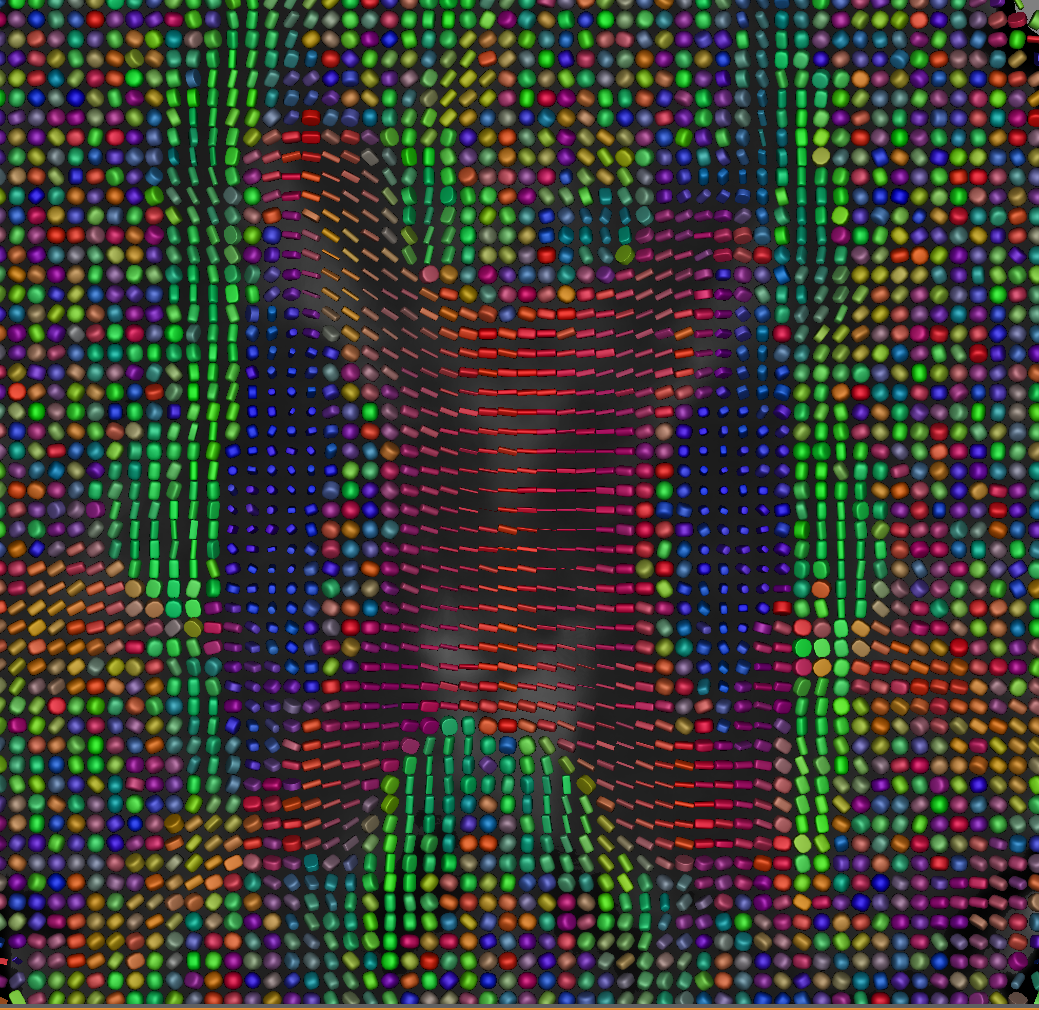
\includegraphics[width=.52\linewidth, angle=0]{figs/Introducao/ex_DTI_Superquadrica.png}
    \label{fig::intro_ex_DTI_glifos}}
    \hfill
    \subfloat[Trato fascículo inferior fronto-occipital (IFOF). A cor predominantemente verde indica sua trajetória, que ocorre na direção anterior-posterior. As linhas são reconstruídas com base no proposto por \citeonline{Weinstein1999} ]{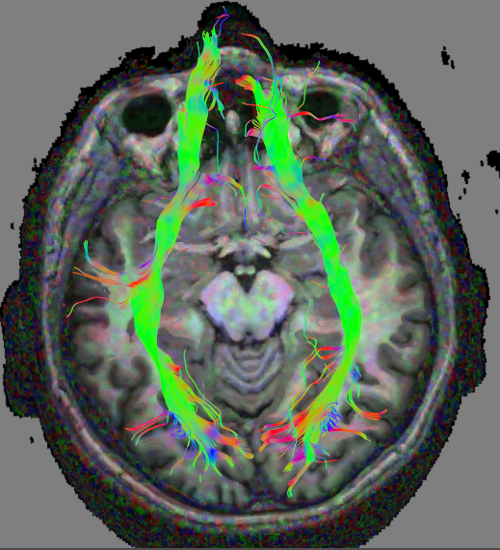
\includegraphics[width=.46\linewidth, angle=0]{figs/Introducao/ex_DTI_tractography.png}
    \label{fig::intro_ex_DTI_tractografia}}
    \caption{Ilustração de resultados de pesquisa na área de visualização em ressonância magnética de difusão utilizando o DTI.}
    \label{fig::intro_ex_DTI}
\end{figure}

%\todo[inline]{ Confira se as literaturas citadas abaixo são relacionadas com glifos e tractografia ... para não tirar o foco. Além de glifos, há várias formas de visualizar os dados dos tensores. Muitos trabalhos visualizam somente FA, ADC, etc.}

% \textcolor{magenta}{
% A partir da visualização de dados extraídos dos tensores, há estudos que buscam inferir sobre a substância branca e utilizá-las em diferentes estudos e diagnósticos. Como alguns exemplos, temos:
% \begin{itemize}
%     \item evidência de correlações de métricas do DTI com a degeneração do cérebro causada pela esclerose lateral amiotrófica e o seu potencial uso como biomarcador \cite{cirillo2012, baek2020};
%     \item diagnósticos de isquemia cerebral aguda em estágios iniciais, o que não é possível com MRI convencionais \cite{dong2004};
%     \item aplicação de métricas e tractografia à redes cognitivas na epilepsia do lobo temporal \cite{leyden2015}
% \end{itemize}
% }

Devido a sua natureza de modelagem, o DTI apresenta limitações. O modelo Gaussiano descreve bem regiões de fibras em que o comportamento de difusão ocorre predominantemente em uma direção. Em pontos que contém múltiplas fibras e que estão dispostas nas mais variadas configurações (por exemplo: cruzamento, bifurcação, fusão, espalhamento, \todo{toque? \textcolor{green}{A expressão que o pessoal usa é essa... o formato das fibras é:  )( é o nome toque não dá essa impressão  }} ``beijo'') o modelo Gaussiano não sintetiza de forma correta o comportamento da difusão, impedindo o cômputo das direções plausíveis para reconstrução de uma fibra de interesse \cite{fillard2011, daducci2014}. Há uma estimativa que entre 66\% a 90\% da substância branca do cérebro contém múltiplas configurações de cruzamento de fibra \cite{descoteaux2015} e a limitação do DTI é um obstáculo para traçar caminhos plausíveis de fibras do cérebro.

Cientes das limitações do DTI, pesquisadores da área propuseram métodos de imageamento com modelos matemáticos mais avançados e descritivos do processo de difusão, os quais passaram a demandar aquisições de \todo{Escreveria qtdes para mostrar "mais".}com uma quantidade maior de amostras de sinais de difusão por \textit{voxel} em comparação às aquisições utilizadas para o DTI. %Tais aquisições são denominadas imagem de difusão por \todo{Ou simplesmente alta resolução como Q-Space Imaging (QSI)}alta resolução angular  (HARDI - \textit{High Angular Resolution Diffusion Imaging}). 
A tese de doutorado de David Tuch \cite{tuch2002} é o trabalho seminal da área.




%  do tensor de difusão representam três direções ortogonais cujos respectivos autovalores representam a magnitude de difusão, que são máximos para restrição de ortogonalidade.

%\todo[inline]{Abstraindo o que você escreveu ... há duas linhas de empenho: visualização dos sinais de difusão por amostra (modelagem local da geometria das fibras) e/ou por fibra (modelagem global da conectividade das amostras). É melhor colocar Fig 1.1 e 1.2 uma ao lado da outra. Facilita análise comparativa.}








%\begin{figure}[ht]
%
%\centering
%\includegraphics[width=.485\linewidth, %angle=00]{figs/Introducao/ex_DTI_Superquadric%a.png}
%\centering
%\caption{Tensor de difusão representado por %glifos superquádricos em uma fatia axial do %cérebro na região do corpo caloso. As cores %representam a direção predominante de difusão %onde vermelho é esquerda-direita, azul é %superior-inferior e verde é %anterior-posterior}
%\label{fig::intro_ex_DTI_Superquadrica}
%\end{figure}

%\begin{figure}[ht]
%\centering
%\includegraphics[width=.485\linewidth, %angle=00]{figs/Introducao/ex_DTI_tractography%.png}
%\caption{Trato fascículo inferior %fronto-occipital (IFOF). A cor %predominantemente verde indica sua %trajetória, que ocorre na direção %anterior-posterior}
%\label{fig::intro_ex_DTI_Tractografia}
%\hfill
%\end{figure}




%\section{Motivação}
%\label{ssec:motivation}



%Uma aquisição DWI é considerada HARDI se há 45 ou mais gradientes de ponderação de difusão. Esta modalidade de aquisição se diferencia de uma aquisição DTI, que costuma possuir entre 6 a 32 direções \cite{descoteaux2015}.


%\todo{\url{https://www.researchgate.net/figure/Sampling-schemes-in-q-space-a-Cartesian-sampling-dedicated-to-diffusion-spectrum_fig3_319558026}}.

Durante a década de 2000, foram propostos métodos de imageamento mais descritivos do processo de difusão que o DTI, como demonstram os trabalhos conduzidos por Tuch \cite{tuch2002}, \cite{TuchQBall2004}, Tournier et al. \cite{tournier2007}, Wedeen et al. \cite{wedeen2005} e Yeh et al. \cite{yeh2010}. Estes métodos tinham como objetivo principal resolver o problema de cruzamento de fibras, assim superando as limitações do DTI. Para diferenciá-los do DTI, neste trabalho chamaremos estes métodos de imageamento de \textsf{métodos alta ordem}.

%Durante a década de 2000, foram propostos métodos de imageamento mais descritivos do processo de difusão que o DTI . Alguns deles consistem na abordagem multi-tensor \cite{tuch2002}, o \textit{Q-Ball Imaging} (QBI) \cite{tuch2002, Kindlmann2004}, \textit{constrained spherical deconvolution} (CSD) \cite{tournier2007}, \textit{diffusion spectrum imaging} (DSI) \cite{tuch2002,wedeen2005} e a amostragem generalizada do espaço Q (GQI - \textit{generalized Q-space sampling}) \cite{yeh2010}.  no qual padrões de fibras subjacentes podem ser inferidos. Para diferenciá-los do DTI, neste trabalho chamaremos estes métodos de imageamento de \textbf{métodos HARDI}.

%Uma ODF, no contexto de DWI, consiste em uma função que associa um conjunto de direções a um valor escalar de difusividade. A representação em forma de glifos para ODFs geralmente consistem na plotagem polar esférica (\textit{spherical polar plot}) de uma ODF min-max normalizada no intervalo [0, 1] \cite{TuchQBall2004}, conforme mostrado na Fig. \ref{fig::ex_glifo_hardi}. Chamaremos esta categoria de glifos neste trabalho de \textbf{glifos ODF}. A renderização interativa desses glifos é um ponto principal deste trabalho e os trabalhos de \citeonline{shattuck2008} e \citeonline{peeters2009, almsick2011} trazem diferentes abordagens para este fim.

%\begin{figure}[h]
%   \centering
%       \addtolength{\leftskip} {-2cm} % increase (absolute) value if needed
%    \addtolength{\rightskip}{-2cm}
%
%    %\vspace*{3mm}
%    \centering
%    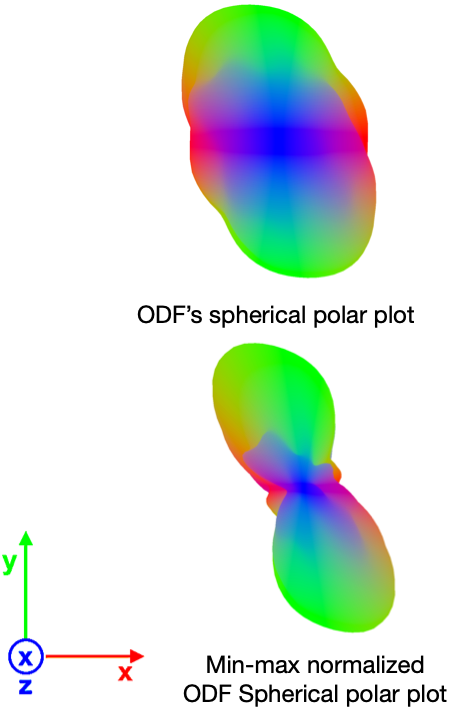
\includegraphics[width=.35\linewidth, angle=0]{figs/Introducao/SphericalMeshModulation.png}
%   \caption{Plotagem polar esférica de uma ODF e sua versão min-max normalizada. A normalização enfatiza a direção dominante de difusão. As cores representam a direção no espaço da superfície, onde o vermelho representa horizontal; verde, a vertical; e azul a direção normal ao plano da tela.}
%    \label{fig::ex_glifo_hardi}
%\end{figure}

\todo[inline]{Não entendi a parte em magenta ... O texto que adicionei não se conecta com ela. "em uma função" é muito vaga. Pelo menos explicita qual tipo de função ... \textcolor{green}{feito!}}

Os métodos usualmente sintetizam os sinais de difusão locais em uma função de distribuição de orientação (\textit{Orientation Distribution Function}, ODF). Estas funções associam uma direção, representada pelo vetor unitário $\mathbf{\hat{u}}$, a um valor escalar de probabilidade $\psi(\mathbf{\hat{u}})$ representativo de difusão \cite{TuchQBall2004, wedeen2005} ou de fibra \cite{Tournier2004DirectEO, tournier2007}. %O primeiro uso desta categoria de funções é documentado por \citeonline{tuch2002}, que mostra que há uma relação de Fourier tridimensional entre os sinais de difusão para a função de difusão. Adicionalmente, o conteúdo direcional da difusão é obtido através através da integração na coordenada radial da função de difusão.

Em ambas as modalidades de ODF, a informação sobre a distribuição de fibras subjacente é extraída de um conjunto de direções feita através do cômputo dos máximos locais das ODFs, nos quais, se aplicados a estas funções reconstruídas a partir de aquisições com uma relação sinal ruído razoável, tendem a ser bem modeladas \cite{fillard2011}.

%\textcolor{red}{Foi demonstrado por ??? \cite{???} que, sem pré-condicionar o comportamento de difusão a um modelo matemático, é possível reconstruir uma função de distribuição, também conhecida por função de densidade de probabilidade, de \todo{orientações?}direções de fibras subjacentes às amostras dos sinais escaneados.} 
%\sout{Os métodos definem transformadas que são aplicadas nas amostras dos sinais de difusão em cada \textit{voxel} em uma função, na qual a distribuição de direções de fibra subjacentes podem ser inferidas.} \textcolor{magenta}{A extração geralmente é feita através da detecção de máximos locais \todo{quais?}destas funções, nos quais, se aplicados sobre aquisições com uma relação sinal ruído razoável, tendem a modelar bem \todo{qual distribuição?}}

A partir da extração de direções fibras subjacentes, tem sido possível gerar tractografias mais coerentes com os tratos reais e que levem em consideração mais nuances do sinal de difusão que o DTI, especialmente em regiões que contém as mais diversas configurações de múltiplas de fibras. Entre os trabalhos que trazem evidências da melhoria da tractografia utilizando métodos de alta ordem, temos:

\begin{itemize}
    \item \citeonline{berman2009} evidencia a melhor reconstrução da conectividade do trato motor na presença de tumor;
    \item \citeonline{bucci2013} evidencia um melhor delineamento do trato corticoespinhal utilizando um método de alta ordem em comparação ao DTI, com validação por estimulação cortical;
    \item \citeonline{kuhnt2013} documenta a melhora da tractografia das radiações ópticas em pacientes com glioma.
\end{itemize}
Mesmo com estas evidências, aquisições e métodos de alta ordem não são popularmente utilizadas clinicamente.


%A partir das ODFs, a direção local de fibras em um \textit{voxel} é modelada de forma adequada pela extração de seus máximos locais \cite{fillard2011}, sendo assim a base para algoritmos de tractografia.  %\textcolor{red}{Porém, (comentar o que falta ainda para popularizar o seu uso clínico em relação a DTI) ...}

No uso clínico, o DTI é ainda muito mais utilizado que métodos alta ordem. As vantagens do DTI se referem a sua aquisição, que requer uma quantidade de dados menor, implicando em um menor tempo para ser feita, e a popularidade de aplicativos que processam DWI por este método de imageamento. Adicionalmente, o DTI demanda uma menor quantidade memória para armazenar parâmetros intrínsecos ao seu método comparados aos métodos de alta ordem e, geralmente o cômputo de parâmetros relacionados em diferentes aplicações, como o próprio cômputo do método, renderização de glifos e tractografia, são computacionalmente menos exigentes. Face a estas dificuldades, a comunidade ainda não desenvolveu  um aplicativo que justifique os tempos de aquisição mais longos \cite{descoteaux2015}.

%Falar de tratos que HARDI resolve e DTI não?

%Em tractografia, tanto baseada em DTI, quanto HARDI, há avanços no entendimento de patologias, como esclerose múltipla, mal de Parkinson, esquizofrenia e derrame \cite{SCHILLING2019194}, e mesmo com essas aplicabilidades, há muitos desafios na área.

%Embora os máximos de ODF obtidas através de métodos HARDI consigam resolver os problemas que dizem respeito à estimativa de direções de fibras de forma local, os métodos não inferem sobre a configuração de fibras -- por exemplo, se as diferentes fibras se cruzam ou se "beijam" \cite{SCHILLING2019194}. A busca por informações adicionais para inferir a natureza da configuração entre múltiplas fibras em diferentes regiões é uma oportunidade ainda em aberto.

%%RELER O ARTIGO DO SCHILING E MOSTRAR OPORTUNIDADES 



%\todo[inline]{Sugiro mencionar aqui o artigo de Schilling et al. mostrando os desafios ainda em aberto.}

\section{Motivação e Objetivos}
\label{ssec:motivation}

Motivados pela maior fidelidade na tractografia dos métodos de alta ordem no mapeamento de tratos em comparação aos tratos reais, nosso grupo de pesquisa tem a intenção de desenvolver um sistema de visualização interativa que mapeia ODFs em glifos e um algoritmo de tractografia interativo baseado na distribuição direcional local de fibras, como ilustrado no fluxograma da Fig. \ref{fig::flowchart_vmtk_hardi}.

Possuímos um ambiente de visualização multimodal para volumes médicos, chamado VMTK-Neuro \cite{VMTKNeuro}. O aplicativo renderiza em tempo real volumes de ressonância magnética (\textit{magnetic resonance imaging} - MRI) e possui ferramentas de exploração 3D para volumes DWI a partir do DTI, no qual há as funcionalidades de renderização interativa de glifos superquádricos e a funcionalidade de tractografia (Fig. \ref{fig::intro_ex_DTI}). Usando o ambiente como infraestrutura, consideramos que o próximo passo para pesquisa no DWI leva em consideração a implementação de um método de alta ordem e a exploração de seus dados objetivando o desenvolvimento de algoritmos de reconstrução de fibras.

\begin{figure}[ht]
   \centering
       \addtolength{\leftskip} {-2cm} % increase (absolute) value if needed
    \addtolength{\rightskip}{-2cm}

    %\vspace*{3mm}
    \centering
    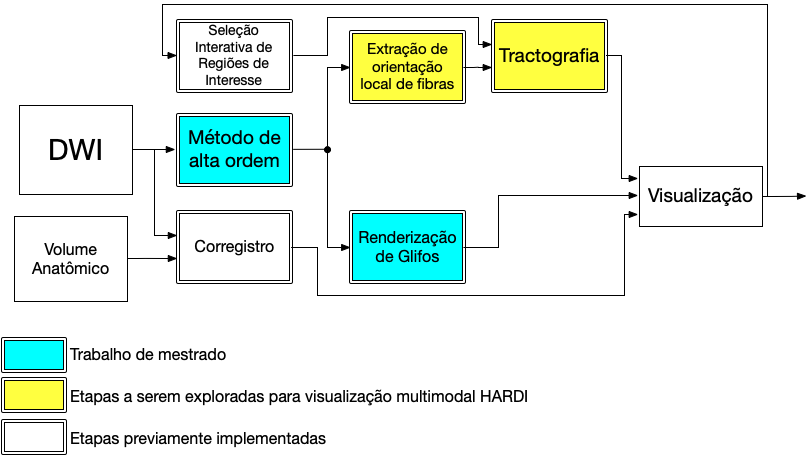
\includegraphics[width=.9\linewidth, angle=0]{figs/Introducao/fluxograma_VMTK_HARDI.png}
    \caption{Fluxograma do ambiente de visualização multimodal para método de alta ordem para DWI. Os capítulos \ref{chapter::metodos_hardi} e \ref{chap::renderizacao_interativa_de_perfis_de_difusao} trazem o detalhamento dos blocos destacados em azul.}
    \label{fig::flowchart_vmtk_hardi}
\end{figure}

%\section{Objetivos}
%\label{sec::objetivos}
Baseados no fluxograma da Fig. \ref{fig::flowchart_vmtk_hardi}, podemos esquematizar os passos para visualização de ODFs em glifos e tractografia em:

\begin{enumerate}
    \item a implementação de um método de imageamento de alta ordem para difusão;
    \item a visualização multimodal dos dados que descrevem a difusão através do método em glifos;
    \item Cômputo da distribuição de fibras subjacentes \textit{voxel} a \textit{voxel}; e
    \item implementação de um algoritmo de tractografia
\end{enumerate}


Cumprindo estes objetivos, estaremos aptos a fazer pesquisas na área de tractografia baseadas em métodos de alta ordem, tanto no que diz respeito a contribuição em métodos e algoritmos, quanto em aplicações clínicas. Sobre métodos de tractografia, \citeonline{SCHILLING2019194} menciona os desafios, oportunidades e limitações nesta área de tractografia, e menciona que a próxima evolução em tractografia há de vir a partir do uso de outras fontes de informação, no qual podemos ter futuras conjecturas para investigação em como podemos utilizar dados co-registrados em adição ao DWI para dar passos adicionais nesta área.

% do uso de métodos de alta ordem em tractografia sobre os desafios da área, temos a intenção de dar 

%Todas as implementações e experimentos do trabalho são realizados no aplicativo VMTK-Neuro (\textit{Visual Manipulation ToolKit for Neuroimages}) \cite{VMTKNeuro}, que é um ambiente de visualização exploratória multimodal multi-plataforma desenvolvida e mantida pelo grupo de pesquisa da Faculdade de Engenharia Elétrica e de Computação da UNICAMP ao qual faço parte. O \textit{software} renderiza em tempo real volumes de ressonância magnética (\textit{magnetic resonance imaging} - MRI) e possui ferramentas de exploração 3D para volumes DWI a partir do DTI, no qual há funcionalidade de exploração local a partir de glifos superquádricos e tractografia (Fig. \ref{fig::intro_ex_DTI}). 



%renderiza em tempo real volumes de ressonância magnética (\textit{magnetic resonance imaging} - MRI) e possui ferramentas de exploração 3D para volumes DWI a partir do DTI, no qual há funcionalidade de exploração local a partir de glifos superquádricos e tractografia (Fig. \ref{fig::intro_ex_DTI}).

%\todo[inline]{A motivação não está bem contextualizada, principalmente depois de ler um parágrafo só sobre as vantagens de DTI no uso clínico. Talvez caiba aqui uma referência em que os autores falam sobre desafios para tornar HARDI popular no uso clínico ... que justificaria o seu trabalho.}

%Nosso grupo de pesquisa tem a intenção de fazer um ambiente exploratório para volumes de difusão através de um método de alta ordem. Neste ambiente, \todo{Isso já não é feito com DTI?}\textcolor{magenta}{um especialista tem total liberdade para construção e análise de forma não invasiva de fibras} e para este fim, desenvolveremos um sistema de visualização interativa de perfis de difusão gerados pelo método de imageamento utilizado em glifos e um algoritmo de tractografia interativo, como ilustrado na fluxograma da Fig. \ref{fig::flowchart_vmtk_hardi}.


Diante destes desafios em aberto, este trabalho aborda a implementação de um método de alta ordem, no qual escolhemos a Amostragem Generalizada no Espaço-Q (\textit{Generalized Q-Sampling Imaging}, GQI) para processamento de volumes de difusão e a proposição de um algoritmo para renderização interativa de glifos que sintetizem as funções obtidas através deste método. Este algoritmo é integrado ao ambiente de visualização multimodal desenvolvido e publicado por \citeonline{voltoline2021}.

Os glifos mais comumente utilizados por pesquisadores da área relacionados a ODFs obtidas através de métodos de alta ordem consistem em suas plotagens polares esféricas. Sua visualização interativa, onde estes objetos são renderizados sobre as suas respectivas regiões no volume melhora a qualidade da pesquisa na área \cite{peeters2009}. A partir dos glifos pode-se inferir visualmente sobre os dados do método de imageamento. A partir disto, o desenvolvedor tem um \textit{feedback} sobre o método de alta ordem implementado, bem como a relação entre método de imageamento e cada aquisição DWI particular.

Adicionalmente, há evidências que o uso de glifos superquádricos posicionados em seus respectivos \textit{voxels} em um ambiente de exploração interativa pode melhorar o processo de escolha de parâmetros iniciais em tractografia \cite{voltoline2021}, o que também é válido para ODFs mapeadas em glifos, visto que esta categoria de glifos permite a inferência sobre cruzamentos de fibra presentes em ODFs, o que não ocorre com superquádricos, dada a limitação do DTI.



%\textcolor{magenta}{A partir dele, pode-se \todo{Para qê inferir?}inferir visualmente sobre o método de imageamento utilizado quanto a sua adequabilidade para com a aquisição utilizada. Adicionalmente, há evidências que o uso de glifos superquádricos posicionados em seus respectivos \textit{voxels} em um ambiente de exploração interativa pode melhorar o processo de escolha de parâmetros iniciais em tractografia \cite{voltoline2021}, o que também é válido para glifos ODF, visto que, esta categoria de glifos permite o usuário ter a informação de cruzamento de fibras, o que não é presente nos superquádricos pela natureza do DTI.}

%Acerca do algoritmo de tractografia, a interação com um especialista é relevante nos seguintes aspectos: queremos que o usuário tenha a liberdade de escolher os tratos a serem analisados e que ele possa inferir e assegurar a plausabilidade das conexões das amostras de múltiplas orientações que métodos HARDI proveem.

%Acerca da natureza do tipo de interatividade que queremos mostrar, evidentemente que somente informações extraídas de um volume de difusão não assegura a plausabilidade de fibras reconstruídas e é desejável que haja ferramentas de interatividade para com um especialista para que ele possa escolher regiões de análise e verificar a plausabilidade de fibras.

%O conhecimento de tratos a partir de DWIs é escasso e há discrepâncias entre especialistas, não apenas na área de difusão, mas também na literatura anatômica \cite{SCHILLING2019194} e é necessária a análise humana para inferir sobre a plausabilidade do que está sendo reconstruído.





%\todo[inline]{Principal motivação é aprimorar a interatividade no processo de reconstrução de uma fibra? Diante dos desafios ainda em aberto, espera-se que, através de uma visualização interativa dos dados de difusão HARDI devidamente pré-processados, um especialista junto com uma máquina construa de forma mais fiel possível, e não-invasiva, as fibras dos tratos (conhecidos e desconhecidos)?}

%\textcolor{red}{No que diz respeito ao método de síntese de orientações das fibras a partir dos volumes HARDI, integramos a sua formulação matemática diretamente no VMTK-Neuro. Os principais critérios para sua escolha se devem a sua adequabilidade em tractografia, sua aplicabilidade em DWIs de baixa resolução angular e simplicidade em relação a quais métodos???.}

%\todo[inline]{Dentre o estado-da-arte da tecnologia HARDI, qual aspecto te chamou atenção e te motivou a desenvolver este trabalho de Mestrado com o objetivo de "implementar e validar um algoritmo (melhor?) de tractografia baseada na técnica de imageamento HARDI"? Na forma como está colocada a sua proposta leva o leitor questionar se o trabalho é simplesmente um exercício do que já se tem.}

%\textcolor{red}{O conhecimento sobre tratos é ainda precário para reconstruí-los integral e automaticamente. É necessária a análise humana para assegurar a plausibilidade das conexões das amostras de múltiplas orientações que a técnica HARDI provê. Para que um especialista possa ter uma visão sucinta e precisa sobre as informações da difusividade local de uma amostra e ajudar uma máquina tomar decisão na ligação desta amostra com as amostras vizinhas para formar uma fibra, é desejável que ele explore de forma interativa tanto os perfis de difusão em cada amostra como as fibras reconstruídas com base nas conjeturas formuladas e reformuladas.}

%\section{Ambiente de Implementação}
%\label{ssec:ambiente}

%Todas as implementações e experimentos do trabalho são realizados no aplicativo VMTK-Neuro (\textit{Visual Manipulation ToolKit for Neuroimages}) \cite{VMTKNeuro}, que é um ambiente de visualização exploratória multimodal multi-plataforma desenvolvida e mantida pelo grupo de pesquisa da Faculdade de Engenharia Elétrica e de Computação da UNICAMP ao qual faço parte. O \textit{software} renderiza em tempo real volumes de ressonância magnética (\textit{magnetic resonance imaging} - MRI) e possui ferramentas de exploração 3D para volumes DWI a partir do DTI, no qual há funcionalidade de exploração local a partir de glifos superquádricos e tractografia (Fig. \ref{fig::intro_ex_DTI}). 





%Na subseção \ref{ssec:vmtk-neuro} do capítulo Materiais e Métodos, ilustramos as ferramentas para DWI como um fluxograma e descrevemos as funcionalidades correlatas ao presente trabalho.

% conforme mostrado no fluxograma da figura \ref{fig::PipelineDTI_tracto}.%\textcolor{red}{escaneados com o protocolo Overplus \cite{Philips} e de rastreamento das fibras para volumes DTI sintetizados a partir de DWIs}\todo{não necessariamente Overplus. Overplus não sintetiza as sequencias de aquisições de DWI que há por aí.}.

%\begin{figure}[ht]
%   \centering
%       \addtolength{\leftskip} {-2cm} % increase (absolute) value if needed
%    \addtolength{\rightskip}{-2cm}
%
%    %\vspace*{3mm}
%    \centering
%    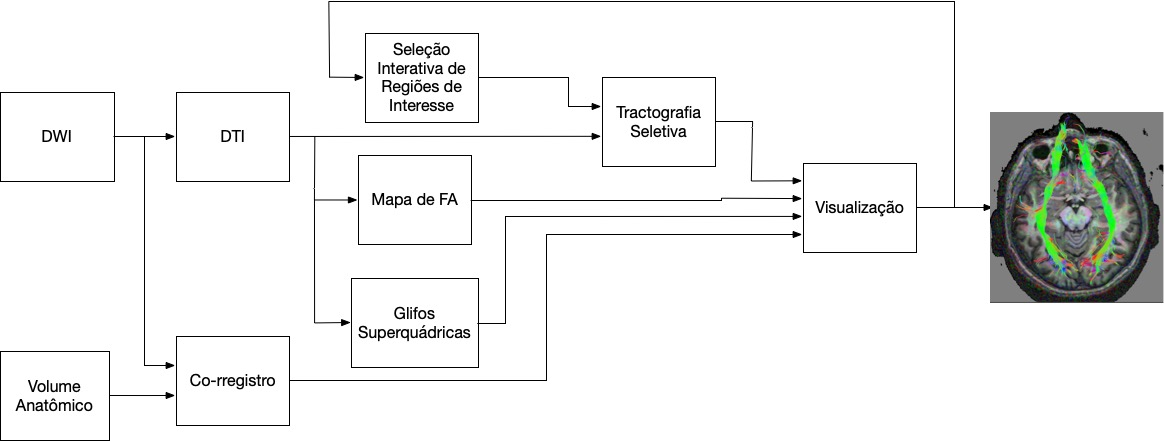
\includegraphics[width=1.0\linewidth, angle=0]{figs/Fluxogramas/PipelineDTI_tracto.jpg}
%    \caption{Fluxograma para tractografia implementado no VMTK-Neuro.}
%    \label{fig::PipelineDTI_tracto}
%\end{figure}

%Estas ferramentas consistem na visualização em tempo interativo de tensores de difusão mapeados em glifos superquádricos \cite{Kindlmann2004} renderizados sobre as suas respectivas amostras (figura \ref{fig::intro_ex_DTI_glifos}), tractografia (figura \ref{fig::intro_ex_DTI_tractografia}) e o corregistro de volumes de difusão com volumes anatômicos T1.

%Na tractografia baseada em DTI, o VMTK-Neuro possui ferramentas de interatividade que possibilitam que o usuário possa inferir sobre as regiões do volume que contém os tratos a serem analisados, bem como filtrar fibras de interesse e eliminar fibras espúrias. Adicionalmente, parâmetros relacionados a reconstrução, que podem diferir de acordo com a região de análise do usuário, também são configuráveis. O algoritmo de tractografia apresenta resultados visuais em tempo interativo para as formas de interação mencionadas.


\todo[inline]{Acho que não foi revisado este capítulo ... Vou parar de ler ... \textcolor{green}{Escrito}}



%\sout{As ferramentas de visualização} O ambiente de visualização multimodal, que integra diferentes modalidades de neuroimagens, incluindo a ressonância de difusão modelada pelo DTI, de forma co-registrada, e, adicionalmente um algoritmo de tractografia interativo, baseado em \citeonline{Weinstein1999}.

%\todo{Motivação?}\textcolor{magenta}{Motivados} pela pesquisa que evidenciam as vantagens da tractografia baseadas em métodos mais avançados em aquisições de alta resolução angular, temos a intenção de fazer a visualização multimodal com DWIs através de algum.




%Adicionalmente, temos a conjectura que os glifos possam ser utilizados para detectar anormalidades nas neuroimagens, bem como servir de suporte visual para escolha de parâmetros iniciais em tractografia, conforme evidenciado em \citeonline{voltoline2021} para superquádricos do DTI.





\section{Contribuição}
\label{sec:contribuicoes}

A contribuição esperada para o presente trabalho dentro do escopo do ambiente exploratório para DWI através de métodos avançados de imageamento é a implementação de um método avançado para difusão, no qual escolhemos a amostragem generalizada no espaço-Q (GQI - \textit{Generalized Q-Space Imaging}) \cite{yeh2010} e a validação de um algoritmo de renderização interativo de glifos que as ODFs geradas pelo método integrado ao ambiente de visualização exploratória multimodal interativo.



%\textcolor{red}{A expectativa é aplicar os resultados na implementação do fluxograma mostrado na Figura ??? no VMTK-Neuro ...}



%\todo[inline]{Sugiro que mostre em algum ponto uma visão geral do fluxo de controle da sua proposta de construção de tractografia a partir de DWIs de alta resolução angular.}

\section{Desafios}
\label{sec::desafios}

Para implementação do sistema, muito da infraestrutura necessária para alcançar os objetivos estabelecidos estão implementadas no VMTK-Neuro para visualização de volumes DWI por DTI. Portanto, muitos dos desafios enfrentados dizem respeito a complexidade matemática e a questões de implementação do método alta ordem e seu esquema de visualização em glifos.

A própria implementação computacional de um método de alta ordem para sintetizar o perfil de difusão é uma tarefa desafiadora. Os métodos demandam uma quantidade de memória da CPU razoavelmente maior que o DTI. Enquanto o DTI é codificado na memória com apenas 6 elementos (matriz 3x3 simétrica), métodos de alta ordem usam dezenas ou centenas de elementos. %Métodos de alta ordem não estabelecem um critério mínimo, entretanto é usual que centenas de elementos sejam utilizados para descreverem o perfil de difusão de forma razoável.

A implementação de um algoritmo de renderização de perfis de difusão em tempo interativo é algo desafiador pela grande quantidade de dados necessários para sintetizar um glifo. Além disso, o algoritmo de renderização é integrado ao pipeline da renderização multimodal volumétrica baseada em \textit{ray-casting} de volumes de ressonância magnética, o que diminui a sua margem de tempo de execução para manter a interatividade.


\section{Organização}
\label{sec:intro_organizacao}

O trabalho está organizado em cinco capítulos. No Capítulo \ref{chapter::metodos_hardi}, descreveremos brevemente sobre as aquisições DWI, a motivação para utilização de métodos de alta ordem para modelar a difusão, detalharemos a implementação do método GQI, tanto no que diz respeito a sua formulação matemática, como a sua implementação computacional; no capítulo \ref{chap::renderizacao_interativa_de_perfis_de_difusao} detalhamos o algoritmo interativo de renderização para glifos que sintetizam ODFs integrado ao VMTK-Neuro atrelado a renderização de um volume \textit{ray-casted}, com sua respectiva validação visual e performance computacional; no Capítulo \ref{chap::renderizacao_de_perfis_de_difusao} detalhamos de forma cronológica os recursos explorados para atingir a interatividade do algoritmo de renderização, bem como os ganhos proporcionados por cada um deles; no Capítulo \ref{chap::conclusao}, concluímos o trabalho e mencionamos oportunidades de trabalhos futuros.


%\chapter{Materiais e Métodos}

%\section{Materiais}






%\subsection{VMTK-Neuro}
%\label{ssec:vmtk-neuro}

%O VMTK-Neuro é um \textit{software} que renderiza em tempo real volumes de ressonância magnética (\textit{magnetic resonance imaging} - MRI) e possui ferramentas de exploração para volumes DWI a partir do DTI, conforme mostrado no fluxograma da figura \ref{fig::PipelineDTI_tracto}. O software utiliza a linguagem de programação em C++ e o OpenGL como API gráfica.

%\begin{figure}[ht]
%   \centering
%       \addtolength{\leftskip} {-2cm} % increase (absolute) value if needed
%    \addtolength{\rightskip}{-2cm}
%
%    %\vspace*{3mm}
%    \centering
%    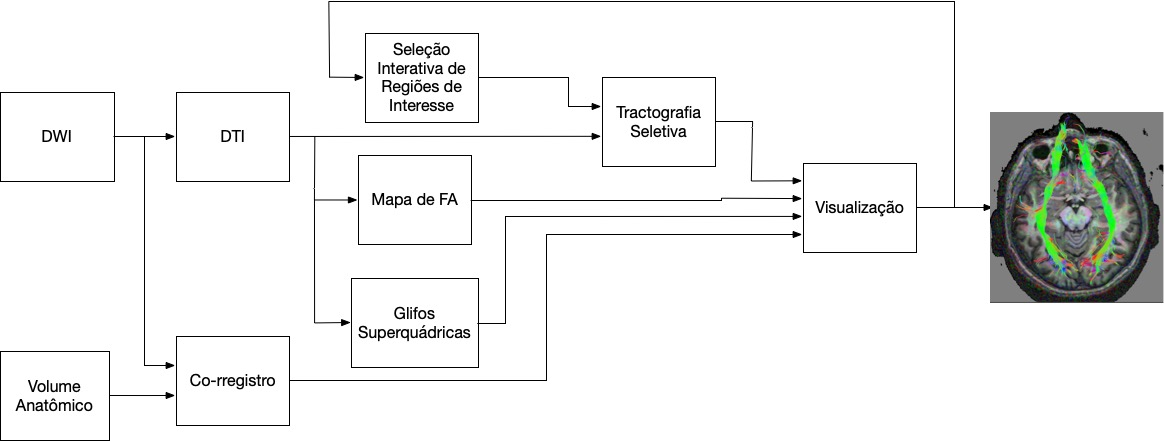
\includegraphics[width=1.0\linewidth, angle=0]{figs/Fluxogramas/PipelineDTI_tracto.jpg}
%    \caption{Fluxograma para tractografia e glifos implementado no VMTK-Neuro.}
%    \label{fig::PipelineDTI_tracto}
%\end{figure}

%Estas ferramentas consistem na visualização em tempo interativo de tensores de difusão mapeados em glifos superquádricos \cite{Kindlmann2004} renderizados sobre as suas respectivas amostras (figura \ref{fig::intro_ex_DTI_glifos}), tractografia (figura \ref{fig::intro_ex_DTI_tractografia}) e o corregistro \cite{ting2014} de volumes de difusão com volumes anatômicos T1 .



%Na tractografia baseada em DTI, o VMTK-Neuro possui ferramentas de interatividade que possibilitam que o usuário possa inferir sobre as regiões do volume que contém os tratos a serem analisados, bem como filtrar fibras de interesse e eliminar fibras espúrias. Adicionalmente, parâmetros relacionados a reconstrução, que podem diferir de acordo com a região de análise do usuário, também são configuráveis. O algoritmo de tractografia apresenta resultados visuais em tempo interativo para as formas de interação mencionadas.


%\subsection{Volumes}

%%%%%VOLUMES UTILIZADOS NOS EXPERIMENTOS


%Temos a intenção de fazer a investigação com dados reais de pacientes do Hospital das Clínicas da UNICAMP, cujo uso foi aprovado pelo comitê de ética CAAE 0893.0.146-000.09, 


%No decorrer do trabalho tínhamos a intenção de usar o volumes do bancos de dados do Hospital das Clínicas da UNICAMP, porém os resultados preliminares em termos de conjuntos de ODFs obtidos não se mostraram adequados, e descartamos o uso. Fizemos um estudo para diagnosticar a natureza do problema, que está detalhado na subseção \ref{ssec::problema_overplus} do apêndice, e concluímos que está relacionado ao conjunto de gradientes de ponderação de difusão utilizado no padrão \textit{Overplus}.


%\section{Métodos}
%\subsection{Interatividade}

%Pela demanda de visualização interativa do VMTK-Neuro, objetivamos que a visualização dos perfis de difusão de glifos ODF para as amostras visíveis na tela aconteça em tempo interativo. Sendo assim, documentaremos os \textit{benchmarks} de ambos sistemas para atestar o cumprimento deste objetivo.

%\subsection{Tractografia}

%A motivação principal desde trabalho nasceu da seguinte pergunta: "como podemos melhorar a tractografia baseada em DTI do VMTK-Neuro?". Neste contexto, iremos comparar a tractografia baseada em DTI implementada no VMTK-Neuro e a tractografia baseada em HARDI em tratos que há a documentação de falhas do DTI e que são resolvidos pela abordagem que utiliza métodos HARDI.

%\todo[inline]{É melhor conversar com o Raphael sobre o uso das imagens da dissertação dele.}


%\textcolor{red}{
\chapter{Imageamento de Difusão Intravoxel}
%\chapter{Imageamento de alta resolução angular para difusão}
\label{chapter::metodos_hardi}
%}

Neste capítulo, trazemos a formulação do conceito de função de distribuição de orientação (ODF - \textit{orientation distribution function}), que é a base para as discussões do capítulo \ref{chap::renderizacao_interativa_de_perfis_de_difusao}, em que detalhamos um esquema de renderização para visualização dos perfis de difusão obtidos através do imageamento. Para que a dissertação seja auto-contida, faremos uma introdução às técnicas de aquisição DWI e aos métodos de síntese de orientações de difusão a partir dos sinais amostrados. Detalharemos o método de reconstrução GQI (\textit{Generalized Q-Sampling Imaging}) que aplicamos neste trabalho de Mestrado.

Na Seção \ref{sec::aquisicao_dwi}, faremos uma breve descrição da sequência de aquisição de um DWI, no que diz respeito as grandezas envolvidas e parâmetros associados, mas sem entrar nos detalhes da física do processo. Na Seção \ref{sec::dti_limitacoes_hardi}, trazemos uma descrição breve do DTI, de ordem 2, suas limitações e a motivação do uso de métodos de mais alta ordem e aquisições de resolução \todo{Falta uma descrição breve da seção de técnicas de ordem maior\\ \textcolor{green}{feito!}}maior. Na Seção \ref{sec::gqi}, descrevemos o principio do método da amostragem generalizada no espaço-Q, no qual mostramos a base teórica, sintetizamos a transformada que leva os sinais de difusão para amostras que sintetizam o comportamento de difusão subjacente através de uma multiplicação matricial, formulamos o domínio de amostragem da transformada e adicionalmente, visando otimizar o uso de memória, exploramos a simetria do comportamento de difusão para diminuir a quantidade de amostras associadas ao domínio armazenadas.

\section{Aquisição DWI}
\label{sec::aquisicao_dwi}
A sequência de pulsos PGSE (\textit{Pulsed Gradient Spin Echo}) é comumente utilizada para inserir a componente de difusão molecular no sinal de MRI, e é normalmente combinada à sequência  EPI (\textit{Echo-Planar Imaging}) de aquisição de MRI. Uma introdução ao assunto pode ser encontrada em \citeonline{DTI_Handbook}. Os fundamentos de imageamento por MRI e sequência de pulsos do EPI podemser encontrados em \citeonline{liang2000}, e a física da difusão e seu imageamento via PGSE integrado ao EPI pode ser encontrado em \citeonline{tuch2002}. Nesta seção, faremos uma introdução às grandezas envolvidas na aquisição, faremos uma introdução ao espaço-Q, e mostramos como é a formulação das amostras de difusão neste espaço a partir de parâmetros acessíveis em aquisições DWI. Usaremos esta formulação para derivação do GQI na seção \ref{sec::gqi}.

Fig. \ref{fig::pgse_ilustrado} ilustra o processo de medição de difusão no qual dois gradientes de ponderação de difusão são aplicados em uma direção $\mathbf{\hat{q}}$ e amplitude $G$. Antes da aplicação do gradiente (período $t_1$), os núcleos de hidrogênios tem seus respectivos \textit{spins} em fase, oscilando na mesma frequência, chamada de frequência de Larmour $f = \gamma \cdot B_0$, onde $\gamma$ é a razão giromagnética do núcleo de hidrogênio e $B_0$ é a magnitude do campo magnético estático principal que excita os \textit{spins} na sequência EPI. O sinal gerado é forte com frequência $f$.

\begin{figure}[ht]

%\subfigcapskip = -5pt
    \centering
    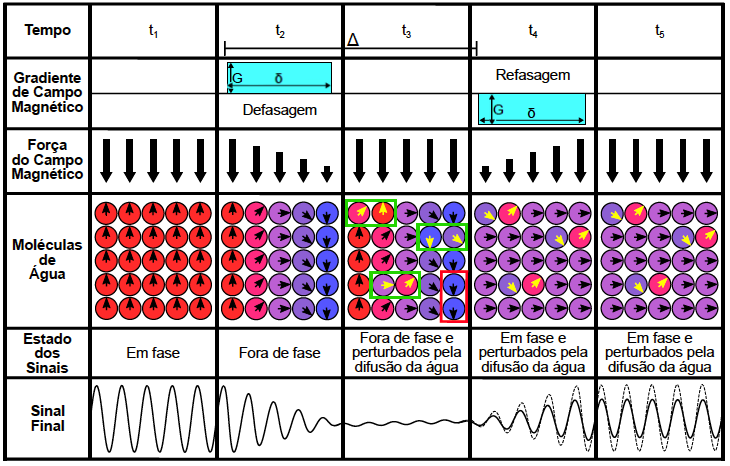
\includegraphics[width=.8\linewidth, angle=0]{figs/HARDI/pgse2.png}
    \caption{Ilustração da medição de difusão das moléculas de água realizada na aquisições DWI nos \textit{scanners} de MRI \\
    Fonte: \cite{voltoline2016}
    }
    \label{fig::pgse_ilustrado}
   \hspace{1pt}
\end{figure}

Em $t_2$, o gradiente de intensidade $G$ em um intervalo de tempo $\delta$ é aplicado. O gradiente é um campo magnético que varia linearmente ao longo da direção $\mathbf{\hat{q}}$ e modifica a frequência de oscilação dos \textit{spins} do núcleo hidrogênio. Quando o gradiente cessa $(t_3)$, os núcleos voltam a ter a mesma frequência de oscilação do período $t_1$, mas com fases diferentes, levando a intensidade do sinal ser enfraquecida.

Depois de um intervalo de tempo $\Delta$ a partir do início da aplicação do primeiro gradiente, o processo de equalizar as fases é inicializado ($t_4$) utilizando um novo gradiente com mesma intensidade e duração, mas com sentido oposto em relação ao primeiro. Os núcleos pertencentes às moléculas que se difundiram na direção $\mathbf{\hat{q}}$ durante o intervalo $\Delta$, destacados em verde na janela de tempo $t_3$, terão suas fases corrigidas de forma a não ter a fase inicial novamente, pois estavam em lugares diferentes no espaço, consequentemente estando sob campos magnéticos diferentes nos instantes de defasagem e equalização de fase. Depois de um intervalo de refasagem, $\delta$, a intensidade do gradiente volta a ser balanceada em $t_5$.
O sinal resultante em $t_5$ é atenuado em relação ao sinal ao intervalo $t_1$ (que está tracejado no instante $t_5$), devido a diferença de fase dos \textit{spins}. Consequentemente, diz-se que o sinal está ponderado em difusão.


A atenuação da ponderação por difusão pode ser configurada através da manipulação dos parâmetros de aquisição  $G$, \todo{Não foi definido $\delta$. \textcolor{green}{ defini como "um intervalo de tempo \delta"}}$\delta$ e $\Delta$. Para sequência PGSE, é comum estas grandezas serem sintetizadas em um fator de ponderação de difusão chamado de valor $b$, que é usualmente expresso em $s/mm^2$. Sua formulação em função dos parâmetros de difusão é dada por \cite{DTI_Handbook}:

\begin{equation}
\label{eq::bvalue}
    b = \gamma^2G^2\delta^2(\Delta - \frac{\delta}{3}).
\end{equation}

Nesta dissertação, usaremos o termo \textsf{volume} ~para referenciar uma imagem 3D composta por imagens 2D e o termo \textsf{fatia} para referenciar estas imagens 2D. Será usado também o termo \textsf{aquisição DWI} quando quisermos referenciar, de uma vez, o conjunto de volumes escaneados numa sessão de aquisição. Nós adotamos o termo \textsf{b0}  para referenciar volumes não-ponderados em difusão em uma aquisição DWI.



A respeito da atenuação gerada pelo gradiente de difusão, uma abordagem simplista no que diz respeito ao cômputo em relação ao sinal não ponderado de difusão, contido no volume b0 é dado pela equação de Stejskal-Tanner \cite{DTI_Handbook}:

\begin{equation}
\label{eq::stanner}
    S(b) = S_0\exp{(-bD)}
\end{equation}
onde $S_0$ é o sinal de difusão sem ponderação, contido no volume b0, S(b) é o sinal de difusão atenuado e $D$ é o coeficiente de difusão aparente (ADC - \textit{Apparent Diffusion Coefficient}), que mensura a quantidade de difusão na direção do gradiente associado ao valor $b$. Observe que o valor $b$ abstrai em um coeficiente os parâmetros de difusão no cômputo da difusão aparente. Esta relação, que não leva em consideração a direção, é válida em difusão livre (Fig. \ref{fig::intro_difusao_isotropica}). Para ambientes em que o ADC depende da orientação $\mathbf{\hat{g}}$ (Fig. \ref{fig::intro_difusao_anisotropica}), é necessária a sua extensão para um ADC$(\mathbf{\hat{g}})$.

\section{Síntese de Direções Intravoxeis}

\subsection{DTI}
%\section{DTI e limitações}
\label{sec::dti_limitacoes_hardi}

\citeonline{Basser1994} propõem o imageamento por tensor de difusão (DTI), que visa modelar o decaimento do sinal de difusão a partir de um modelo Gaussiano: 
\begin{equation}
\label{eq::stanner}
    S(\mathbf{\hat{g}}, b) = S_0\exp{(-b\mathbf{\hat{g}^T}\mathbf{D}\mathbf{\hat{g}})}, 
\end{equation}
no qual podemos sintetizar o modelo pelo tensor de difusão $\mathbf{D}$ de ordem 2 e representá-lo por uma matriz 3x3 simétrica:

\begin{equation}
\label{eq::tensor}
\mathbf{D} = 
\begin{bmatrix}
D_{xx} & D_{xy} & D_{xz} \\ 
D_{xy} & D_{yy} & D_{yz} \\ 
D_{xz} & D_{yz} & D_{zz}  
\end{bmatrix}
\end{equation}
e o coeficiente de difusão aparente de difusão $D(\mathbf{\hat{g}})$ é modelado por:

\begin{equation}
\label{eq::dti_model}
    D(\mathbf{\hat{g}}) = \mathbf{\hat{g}^T}\mathbf{D}\mathbf{\hat{g}}.
\end{equation}
%e o decaimento da difusão, derivado da Eq. \ref{eq::stanner}, se torna uma função dada por:

Observe que para cômputo do modelo, o DTI precisa de pelo menos seis volumes de difusão, para resolver o sistema de equações de seis incógnitas do tensor de difusão a partir do ADC $D(\mathbf{\hat{g}})$, onde $\mathbf{\hat{g}} = [g_x, g_y, g_z]^T$, mostrado na Eq. \ref{eq::sistema_dti}:

\begin{equation}
\label{eq::sistema_dti}
\frac{1}{b}\ln{\frac{S_0}{S(\mathbf{\hat{g}})}}=D_{x x} g_{x}^{2} +D_{y y} g_{y}^{2}+D_{z z} g_{z}^{2}+2 D_{x y} g_{x} g_{y} +2 D_{x z} g_{x} g_{z}+2 D_{y z} g_{y} g_{z}
\end{equation}
onde o termo à esquerda é o cômputo do coeficiente aparente de difusão para o sinal $S(\mathbf{\hat{g}})$, derivado da Eq. \ref{eq::stanner} e à direita, expandimos a operação mostrada na Eq. \ref{eq::dti_model}. Na prática, as aquisições DTI tem entre 6 e 32 volumes ponderados por difusão e um volume b0. 

Usualmente, a informação referente ao processo de difusão é extraída dos três autovetores e autovalores da matriz $\mathbf{D}$ (Eq. \ref{eq::tensor}), onde a direção da fibra é usualmente paralela a direção do autovetor associado ao maior autovalor.
Porém, o DTI apresenta limitações, que se devem ao próprio modelo Gaussiano utilizado.

O modelo descreve bem regiões de fibras em que o comportamento de difusão ocorre predominantemente em uma direção. Em pontos que contém múltiplas fibras e que estão dispostas nas mais variadas configurações (por exemplo: cruzamento, bifurcação, fusão, espalhamento, "beijo") o modelo Gaussiano não sintetiza de forma correta o comportamento da difusão, impedindo o cômputo das direções plausíveis para reconstrução de uma fibra de interesse \cite{fillard2011, daducci2014}. Há um estimativa de que entre 66\% a 90\% da substância branca do cérebro contém múltiplas configurações de cruzamento de fibra \cite{descoteaux2015} e a limitação do DTI é um obstáculo para modelar as direções de fibras subjacentes de forma adequada dentro de um \textit{voxel}.

\subsection{Métodos de alta ordem}

Devido às limitações do DTI para inferir sobre a substância branca do cérebro na resolução de cruzamento de fibras, houve uma agenda de pesquisa que começa no início da década de 2000 para distinguir múltiplas orientações numa amostra, e consequentemente houve uma demanda por mais amostras de sinais de difusão por \textit{voxel} nas aquisições DWI. %denominadas de imageamento difusão de alta resolução angular para difusão (HARDI - \textit{high angular resolution diffusion imaging}). Tipicamente aquisições HARDI \textit{single-shell} contém 45 volumes ponderados por e $1000 \leq b \leq 4500$ $s/mm^2$.

Houve mais de cem artigos que propuseram métodos de imageamento para transformação do sinal de difusão para o seu perfil de densidade de probabilidade de direções de difusão de fibras entre 2000-2010 \cite{descoteaux2015}. Os métodos consistem essencialmente na síntese do sinal de difusão em funções de distribuição de orientações (ODF) que dão a possibilidade de inferir sobre a distribuição de fibras subjacentes. Uma ODF consiste em uma associação entre um conjunto de direções, usualmente representadas por um vetor unitário $\mathbf{\hat{u}}$ (ou par $(\theta, \phi)$ em coordenadas esféricas), em um valor escalar $\psi(\mathbf{\hat{u}})$, representativo da probabilidade de difusividade em $\mathbf{\hat{u}}$. Em geral, estes métodos podem ser categorizados de duas formas de acordo com a natureza da técnica de transformada do sinal de difusão para a ODF: técnicas de misturas (\textit{mixture models techniques}) e técnicas livres de modelo, que abrange o GQI.

Estes métodos requerem uma quantidade maior de volumes ponderados por difusão em um DWI, além de maiores valores $b$. Tipicamente, a quantidade de gradientes de ponderação por difusão é acima de 45, e $1000 \leq b \leq 4500s/mm^2$ \cite{descoteaux2015}. Comumente, aquisições DWI possuem um valor $b$ fixo para os volumes ponderados por difusão. Estas aquisições são chamadas de \textit{single-shell} porque suas amostras estão contidas em uma esfera no espaço-Q (Seção \ref{metodos_livres_de_modelo}). Aquisições \textit{single-shell} adequadas para métodos de alta ordem são chamadas de imagem de difusão de alta resolução angular (\textit{High Angular Resolution Diffusion Imaging, HARDI}).

Em adição às aquisições HARDI \textit{single-shell}, há mais duas que valem mencionar: aquisições HARDI \textit{multi-shell}, no qual as aquisições são feitas para múltiplos valores $b$, tipicamente dois ou três, que constam no banco de dados do projeto Connectomme \cite{essen2012} e a aquisição cartesiana no Espaço-Q, que normalmente é associada ao método \textit{Diffusion Spectrum Imaging}, e é inviável clinicamente (Seção \ref{metodos_livres_de_modelo}). \citeonline{cheng2018} discutem e formulam aquisições \textit{single-shell} e \textit{multi-shell} HARDI.


\subsubsection{Técnicas de misturas}

Técnicas de misturas assumem que o sinal de difusão medido para um \textit{voxel} é a soma dos sinais gerados por cada população de fibra presente nele \cite{tournier2011}. Como exemplos, há a abordagem multi-tensor, também presente na tese de doutorado de \citeonline{tuch2002}, e a abordagem por deconvolução esférica, proposta originalmente por \citeonline{Tournier2004DirectEO}.

A abordagem multi-tensor modela a difusão como uma soma ponderada de modelos Gaussianos, com diferentes tensores associados a cada um. Enquanto na abordagem por deconvolução esférica, parte-se da premissa de que o sinal de difusão é gerado a partir da resposta da fibra ao gradiente de ponderação de difusão e este fenômeno é representado por uma convolução da função de distribuição de orientação de fibras (fODF) por uma função resposta para uma fibra única. Assim, a fODF é reconstruída a partir de uma técnica de deconvolução. O aplicativo MRTrix\footnote{Disponível em: https://www.mrtrix.org/} utiliza a abordagem \textit{constrained spherical deconvolution} \cite{tournier2007} para sintetizar o sinal de difusão em uma fODF.

\subsubsection{Métodos livres de modelo}
\label{metodos_livres_de_modelo}

\todo{O que é $\mathbf{\hat{q}}$?}

Nos métodos livres de modelo, os sinais de difusão são modeladas como amostras no espaço-Q em coordenadas $\mathbf{q}$. Os sinais de difusão $W(\mathbf{r}, \mathbf{q})$ no \textit{voxel} $\mathbf{r}$ são amostrados no ponto representado por\footnote{\citeonline{tuch2002} representa esta relação por $\mathbf{q} = (\gamma G \delta)\cdot \mathbf{\hat{q}}$} \cite{yeh2010}:

\begin{equation}
    \label{eq::ting}
    \mathbf{q} = \frac{\gamma G \delta}{2\pi} \cdot \mathbf{\hat{q}},
\end{equation}
onde $\mathbf{\hat{q}} = \mathbf{q}/|\mathbf{q}|$ é a direção do gradiente de ponderação de difusão, $\gamma$ é a razão giromagnética do núcleo de hidrogênio $G$ e $\delta$ são parâmetros do PGSE (Fig. \ref{fig::pgse_ilustrado}).

A partir dessas amostras, métodos de imageamento, como o \textit{Diffusion Spectrum Imaging} (DSI), \textit{Q-Ball Imaging} e GQI, são utilizados para inferir sobre o perfil de difusão, ou  a distribuição de probabilidade direcional de fibras \textit{voxel} a \textit{voxel}, fazendo uso da relação de Fourier entre o $W(\mathbf{r}, \mathbf{q})$ e o propagador de difusão $p(\mathbf{r}, \mathbf{u})$. O propagador de difusão é uma função que gera a probabilidade de deslocamento $\mathbf{u}$ durante um tempo de difusão $t$. A relação entre ambas está ilustrada na Eq. \ref{eq::propagator}.

%O propagador de difusão $p(\mathbf{r}, \mathbf{u})$ é uma função que gera a probabilidade de deslocamento $\mathbf{u}$ durante um tempo de difusão $t$:

%\todo[inline]{Explique o operador $\mathfrak{F}^{-1}$.}
\begin{equation}
\label{eq::propagator}
    p( \mathbf{u}, t) =\int W(\mathbf{q}, t) \exp (i2 \pi \mathbf{q} \cdot \mathbf{u}) d \mathbf{q}
\end{equation}

% \begin{equation}
% \int_{\mathbf{q} \in Q} W(\mathbf{q}, t) \exp (i2 \pi \mathbf{q} \cdot \mathbf{R}) d \mathbf{q}
% \end{equation}

Substituindo a Eq. \ref{eq::bvalue} na Eq. \ref{eq::ting} e definindo $\tau = \Delta - \delta/3$, chegamos a uma relação em que mostra que a amostragem $\mathbf{q}$ como função dos valores $b$.

\begin{equation}
\label{eq::qspace_bvalue}
\mathbf{q} = \frac{1}{2\pi}\sqrt{\frac{b}{\tau}} \mathbf{\hat{q}}
\end{equation}

A partir do propagador de difusão, a função de distribuição de orientação de difusão (\textit{Diffusion Orientation Distribution Function}, dODF) $\Psi(\mathbf{\hat{u}})$ para a direção $\mathbf{\hat{u}}$ é capturada a partir do conteúdo do angular, e esta função nos permite sintetizar a distribuição de fibras subjacente. Sua relação com o propagador de difusão está na Eq. \ref{eq::dodf_propagador}.

\todo[inline]{Aqui você deu novamente um pulo de gato. O que é $\mathbf{\hat{u}}$? E onde foi parar $t$ da Eq. \ref{eq::propagator}? O texto acima não é claro ...}
\begin{equation}
\label{eq::dodf_propagador}
\Psi(\mathbf{\hat{u}})=\int_{0}^{\infty} p(\rho  \mathbf{\hat{u}}) \rho^2 \mathrm{~d}\rho
\end{equation}

\todo[inline]{Sugiro que insira no parágrafo abaixo o que conversamos: DSI faz aquisições diretas do espectro médio dos deslocamento de \textit{spins} amostrados em intervalos regulares de direções $\mathbf{u}$ e de ponderações em difusão $b$ no espaço-Q,  e faz uso das Eqs. \ref{eq::qspace_bvalue} e \ref{eq::dodf_propagador} para recuperar (diretamente) os sinais no espaço $R^3$ via transformadas inversas de Fourier. Requer multiplos valores b e múltiplos gradientes. E dar uma ideia em que consistem as aquisições menos demandantes, porém equivalentes, entre as quais estão GQI que você vai detalhar na próxima seção.}

O DSI \cite{wedeen2005} faz o mapeamento mostrado nas Eq. \ref{eq::qspace_bvalue} e \ref{eq::dodf_propagador} e demanda por uma aquisição com muitos volumes de difusão. As amostragem no espaço-Q para este método são tipicamente uniformemente espaçada nas três dimensões e necessitam de muitos volumes ponderados por difusão (515 volumes \cite{wedeen2005}) e gradientes de ponderação de difusão fortes ($0 \leq b \leq 17000 s/mm^2$), o que é demandado no cômputo da transformada discreta de Fourier 3D. Devido a isto, outros métodos surgem com o objetivo derivar transformações para dODFs com uma menor demanda na quantidade de volumes ponderados por difusão adquiridos, e adequados para aquisições HARDI.

O \textit{Q-Ball Imaging} é o primeiro deles, no qual \citeonline{TuchQBall2004} mostra que em uma aquisição HARDI \textit{single shell}, é possível obter uma versão suavizada da dODF do DSI aplicando a transformada de Funk-Radon na esfera no Espaço-Q que contém o sinal de difusão.

%O \textit{Q-Ball Imaging} \cite{TuchQBall2004} é um destes métodos e o primeiro a ser proposto após o DSI. \citeonline{TuchQBall2004} prova que a uma versão suavizada da dODF pode ser computada através da Transformada de Funk-Radon aplicada em uma esfera no espaço-Q. Este método é implementado na biblioteca FSL\footnote{Disponível em: https://fsl.fmrib.ox.ac.uk/fsl/fslwiki/FSL}.


Neste trabalho, escolhemos o GQI para reconstruir ODFs a partir dos esquemas de aquisição de alta resolução angular pelas seguintes características \cite{yeh2010}:

\begin{enumerate}
    \item ser aplicável em categorias de aquisição com múltiplos valores $b$;
    \item bom desempenho em volumes de mais baixa resolução angular;
    \item ter parâmetros de regularização e filtragem integrados ao método, o que é necessário para o cômputo das informações direcionais das fibras subjacentes.
\end{enumerate}

Um ponto importante no processo de escolha é referente à adequabilidade em tractografia. No seu trabalho sobre comparações de diferentes métodos de imageamento em tractografia, \citeonline{daducci2014} concluíram que não há métodos que se sobressaem em relação a outros nas mais diferentes condições experimentais.

%O DSI \cite{wedeen2005} - proposto originalmente em 2000 - explora e sintetiza uma função de orientação de orientação de através da relação de Fourier entre o sinal de difusão no espaço-Q e a aquisição

















%consiste em um mapeamento das amostras de difusão em um ponto contido em uma aquisição DWI em um modelo gaussiano, que é sintetizada por tensor de ordem 2, representado por uma matriz 3x3 simétrica (Eq. \ref{eq::tensor}). Para seu cômputo, o DTI necessita de no mínimo seis volumes ponderados por difusão em adição a um $b0$, nos quais geram um sistema para cômputo dos seis coeficientes do tensor. Na prática, os volumes DWI escaneados para serem usados com este método, que é predominante no uso clínico, varia entre 6 e 32 \cite{descoteaux2015}.




%Entretanto, o método apresenta limitações \textcolor{red}{como já destacado na seção \ref{sec:introducao}.}



%e o termo \textsf{resolução angular} \sout{com} \textcolor{red}{à} quantidade de volumes ponderados por difusão em uma aquisição DWI. 

%\todo[inline]{DTI assume que a função densidade de probabilidade é Gaussiana enquanto a representação no espaço q (Q-space imaging) não faz nenhuma suposição quanto a um modelo para a função densidade de probabilidade. As funções de difusão no espaço Q são adquiridas diretamente através da amostragem dos sinais de difusão num reticulado cartesiano 3D. Amostragens sobre calotas esféricas (\textit{spherical shell}) são conhecidas como HARDI. É mostrado que HARDI pode ser transformado em Q-ball imaging, também sem condicionamento a um modelo. Veja \cite{TuchQBall2004}. As explicações que se seguem estão confusas. Parece que você colocou num pacote QSI e HARDI/QBI.}



% \textcolor{magenta}{
% A respeito dos valores $b$ utilizados em uma aquisição DWI, e como utilizá-los no espaço-Q, há normalmente três estratégias de amostragens para a aquisição:
% \begin{enumerate}
%     \item amostragem cartesiana, onde as amostras são igualmente espaçadas no espaço-Q em um espaço cartesiano tridimensional e que é usualmente associado ao imageamento de espectro por difusão (DSI) \cite{wedeen2005};
%     \item amostragem \textit{single-shell}, que consiste na amostragem feita para um valor b constante, que está contido numa esfera no espaço-Q;
%     \item amostragem \textit{multi-shell}, que consiste na amostragem que consiste em diferentes conjuntos de pontos contidos em mais de uma esfera, que se referem a uma quantidade no espaço-Q.
% \end{enumerate}
% }



%!! ILUSTRAR SINGLESHELL- MULTISHELL  e CARTESIANA!!

%Dado um conjunto de amostras de sinais de difusão no espaço-Q, há diversas técnicas para descrever o processo de difusão \textit{voxel} a \textit{voxel} sumarizá-los em potenciais caminhos de fibras, sendo o DTI \cite{Basser1994} a mais utilizada.


%\section{DTI, limitações e HARDI}
%\section{Estimativa de Orientações de Difusão}
%\label{sec::dti_limitacoes_hardi}
%\todo[inline]{Sugiro que façs aqui uma espécie de survey dos métodos ... Fica a seu critério a classificação ... pode ser por forma de amostragem como em \url{https://www.researchgate.net/publication/319558026_High_Angular_Resolution_Diffusion_Imaging_HARDI/link/59e88db8a6fdccfe7f8e8a4f/download} ... Sugiro que poderia fazer um merge com capítulo 3.}

%Na aquisição do DWI, é escaneado um conjunto de volumes em que cada um possui a ponderação de único gradiente de difusão associado a um valor-b\footnote{O valor-b é uma métrica de sensitividade para difusão e é função de parâmetros da aquisição do DWI, como função da intensidade, duração e o intervalo de tempo dos gradientes de ponderação de difusão. Quanto maior o seu valor, maior o decaimento do sinal relativo à difusão.}, e, adicionalmente, um ou mais volumes sem ponderação de gradiente, denominado volume b0. A quantidade de volumes ponderados para diferentes direções de gradiente é denominada de resolução angular. Técnicas para sumarizar os sinais coletados em informações de potenciais caminhos de fibras nervosas são objeto de pesquisa desde o início dos anos 90 \cite{descoteaux2015}.



%\sout{A limitação do DTI acerca da possibilidade de inferir sobre fibras subjacentes é vinculada a modelagem da difusão ao modelo Gaussiano. O modelo descreve bem regiões de fibras em que o comportamento de difusão ocorre predominantemente em uma direção. Em pontos que contém múltiplas fibras e que estão dispostas nas mais variadas configurações (por exemplo: cruzamento, bifurcação, mistura, "beijo") o modelo gaussiano não sintetiza de forma correta o comportamento da difusão, impedindo o cômputo das direções plausíveis para reconstrução de uma fibra de interesse \cite{fillard2011, daducci2014}. Há um estimativa que entre 66\% a 90\% da substância branca do cérebro contém múltiplas configurações de cruzamento de fibra \cite{descoteaux2015} e a limitação do DTI é um obstáculo para modelar as direções de fibras subjacentes de forma adequada.}

%\todo[inline]{Não há Q-space imaging como uma proposta alternativa para DTI?}





%As técnicas livres de modelo buscam \sout{formular} uma \sout{representação para} formulação da \sout{função de} difusão \textcolor{red}{em função do seu perfil angular $\psi(\mathbf{\hat{u}})$,} explorando a relação de Fourier \cite{tuch2002} do sinal de difusão $W(\mathbf{r}, \mathbf{q})$\sout{ para obtenção de características da difusão em seu perfil angular $\psi(\mathbf{\hat{u}})$}. Entre os métodos \sout{foram} propostos, \textcolor{red}{destacam-se} o DSI \textcolor{red}{(\textit{Diffusion Sampling Imaging})} \cite{wedeen2005}, proposto originalmente em 2000 e presente na tese de doutorado de \citeonline{tuch2002}, juntamente com o QBI \textcolor{red}{(\textit{Q-ball Imaging})}, proposto em \citeonline{TuchQBall2004} \sout{em sua forma de artigo}, e o GQI \textcolor{red}{(\textit{Generalized Q-sampling Imaging})} \cite{yeh2010}\sout{ exemplificam esta categoria de métodos}.


%!!Porque geram ODFs?

%Estes métodos geram uma ODF a partir do sinal de difusão. Geralmente ODFs não possui a restrição quanto a regressão uma função tridimensional que o DTI possui e portanto conseguem ser mais descritivos do processo de difusão e gerar boas aproximações das fibras subjacentes, especialmente em cruzamentos \cite{daducci2014}.

% e evidentemente precisamos fazer uma seleção dos quais deles são mais relevantes para o nosso trabalho.

%Há diferentes aplicativos livres\textcolor{red}{, ligados a grupos de pesquisa,} que \sout{utilizam métodos HARDI}\textcolor{red}{não assumem modelos gaussianos} para processamento de DWI\sout{, que estão ligados a grupos de pesquisa na área,}. \sout{alguns destes aplicativos utilizam} \textcolor{red}{Encontram-se implementados} o GQI (DSI-Studio\footnote{Disponível em: http://dsi-studio.labsolver.org}), QBI (FSL\footnote{Disponível em: https://fsl.fmrib.ox.ac.uk/fsl/fslwiki/FSL}, FiberNavigator\footnote{Disponível em: https://scilus.github.io/fibernavigator/}), ambos métodos livres de modelo, e o \textit{constrained spherical deconvolution} \cite{tournier2007} (MRTrix\footnote{Disponível em: https://www.mrtrix.org/}), que é uma abordagem de deconvolução esférica.




%A grande desvantagem do GQI implementado na forma proposta por \citeonline{yeh2010} ocorre no uso de memória. A codificação de ODFs é feita por amostras e requer uma grande quantidade de memória, usualmente nas centenas de números por \textit{voxel}. Métodos que armazenam os dados como coeficientes de função base, como o QBI formulado por \citeonline{descoteaux2007_QBI} e o CSD \cite{tournier2007} tendem a utilizar menos memória.

\subsection{Amostragem Generalizada no Espaço Q}

Nesta seção faremos uma breve apresentação do método GQI (\textit{Generalized Q-sampling Imaging}), a sua fundamentação teórica, na qual mostraremos a transformação do sinal de difusão $W(\mathbf{r},\mathbf{q})$ para ODF através de uma multiplicação matricial, e a discretização uniforme do domínio de amostragem da ODF.

%o método de reconstrução de funções de densidade de probabilidade de difusão em relação às diferentes orientações que usaremos para reconstruir ODF (\textit{Orientation Distribution Function}).

\label{sec::gqi}
\subsubsection{Formulação}

O GQI é um método de modelo livre, derivado da relação de Fourier entre o sinal de difusão $W(\mathbf{r},  \mathbf{q})$ no \textit{voxel}, de coordenadas $\mathbf{r}$, no espaço-Q, e o deslocamento dos \textit{spins} devido à difusão, modelado pela função de distribuição de \textit{spins} (\textit{Spin Distribution Function}, SDF) $\psi_Q(\mathbf{r}, \mathbf{\hat{u}})$.

Para isso, o método explora a relação de Fourier em três dimensões entre o sinal de difusão $W(\mathbf{r}, \mathbf{q})$ e a função de densidade de \textit{spins} $Q(\mathbf{r}, \mathbf{R})$:

\begin{equation}
\label{eq::spin_diffsignal_1}
    Q(\mathbf{r}, \mathbf{R}) =
    \int \! W(\mathbf{r}, \mathbf{q})e^{-i2\pi \mathbf{q}\cdot \mathbf{R} } \,\mathrm{d}\mathbf{q} .
\end{equation}

Como $Q(\mathbf{r}, \mathbf{R})$ é real e $W(\mathbf{r}, \mathbf{q})$ é simétrica, podemos considerar a parte real da transformada, reduzindo a expressão em:

\begin{equation}
\label{eq::spin_diffsignal_2}
    Q(\mathbf{r}, \mathbf{R}) =
     \int \! W(\mathbf{r}, \mathbf{q})\text{cos}(2\pi \mathbf{q}\cdot \mathbf{R}) \,\mathrm{d}\mathbf{q} .
\end{equation}

Por outro lado, podemos estimar a quantidade de \textit{spins} que se submetem a difusão em uma direção $\mathbf{\hat{u}}$ através da integração da função $Q(\mathbf{r}, \mathbf{R})$ nesta direção, o que resulta em:
\begin{equation}
\label{eq::sdf_spin}
    \psi_Q(\mathbf{r}, \mathbf{\hat{u}}) =
   \int_{0}^{L_{\Delta}} Q(\mathbf{r}, L\mathbf{\hat{u}})\!  \,\mathrm{d}L , 
\end{equation}
onde $L_\Delta$ é a distância de difusão na direção  $\mathbf{r}$.

Combinando as Eq. \ref{eq::spin_diffsignal_2} e \ref{eq::sdf_spin}, obtemos a relação entre os sinais de difusão $W(\mathbf{r}, \mathbf{q})$ e $\psi_Q(\mathbf{r}, \mathbf{\hat{u}})$:
\begin{equation}
\label{eq::sdf_continuous_1}
    \psi_Q(\mathbf{r}, \mathbf{\hat{u}}) =
    \int_{0}^{L_{\Delta}}\int \! W(\mathbf{r}, \mathbf{q}) \text{cos}(2\pi L_{\Delta} \mathbf{q} \cdot \mathbf{\hat{u}}) \,\mathrm{d}\mathbf{q} \mathrm{d}L .
\end{equation}

Integrando em $L$, obtemos $\psi_Q(\mathbf{r}, \mathbf{\hat{u}})$ em função do sinal de difusão: 
\begin{equation}
\label{eq::sdf_continuous_2}
    \psi_Q(\mathbf{r}, \mathbf{\hat{u}}) =
    L_{\Delta} \int \! W(\mathbf{r}, \mathbf{q}) \text{sinc}(2\pi L_{\Delta} \mathbf{q} \cdot \mathbf{\hat{u}}) \,\mathrm{d}\mathbf{q} ,
\end{equation}
onde $\text{sinc}(x) = \text{sin}(x)/x$ para todo $x$ real, exceto $0$ e $\text{sinc}(0) = 1$.

Assumindo que a área de quadratura seja constante $A_q$ na discretização da Eq. \ref{eq::sdf_continuous_2}, chegamos na SDF medida  chegamos na SDF medida $\psi_m(\mathbf{r}, \mathbf{\hat{u}})$: 


\begin{equation}
\label{eq::sdf_discrete_1}
    \psi_m(\mathbf{r}, \mathbf{\hat{u}}) =
     A_qL_{\Delta}\sum_{\mathbf{q} \in \mathbf{Q}} W(\mathbf{r}, \mathbf{q})\text{sinc}(2\pi L_{\Delta} \mathbf{q}\cdot\mathbf{\hat{u}}),
\end{equation}
onde $\mathbf{Q}= [
\mathbf{q}_1,
\mathbf{q}_2,
\mathbf{q}_3, ...,
\mathbf{q}_T
]$ corresponde às $T$ amostras no espaço-Q.

Observe que a distância de difusão ajusta a contribuição de cada $W(\mathbf{r}, \mathbf{q})$ no cômputo de $\psi_m(\mathbf{r}, \mathbf{\hat{u}})$ e funciona como um parâmetro de regularização. Se $L_{\Delta}$ tende a infinito, a função de distribuição irá se comportar como um impulso na origem, gerando um $\psi_m(\mathbf{r}, \mathbf{\hat{u}})$ fortemente ponderado pelas direções de $\mathbf{q}$ ortogonais a $\mathbf{\hat{u}}$. Um $L_{\Delta}$ pequeno implica em uma maior ponderação para coeficientes que não são ortogonais a $\mathbf{\hat{u}}$, o que atua como uma filtragem. No caso extremo, $L_{\Delta} = 0$, implica que todos os pesos aplicados para cômputo de ODFs em todas as direções $\mathbf{\hat{u}}$ se tornem iguais.

Considerando que a distribuição da difusão seja Gaussiana, a distância de difusão é dada por $L_{\Delta}=(6D\tau)^{1/2}$, onde $D$ é o coeficiente de difusão da água na temperatura do corpo e $\tau = \Delta - \delta/3$, que correspondem aos parâmetros de aquisição mostrados em Fig. \ref{fig::pgse_ilustrado}. 
Tipicamente, assume-se $D = 3.0*10^{-3} mm^2/s$ \cite{yeh2019_DSI}. Podemos ponderar $L_{\Delta}$ por um fator $\sigma$, isto é, $L_{\Delta} = \sigma(6D\tau)^{1/2}$. Para $\sigma$ = 1.3, $80\%$ da difusão é considerada no cômputo da $\psi_Q(\mathbf{r}, \mathbf{\hat{u}})$.

Substituindo $L_{\Delta}$ por $\sigma(6D\tau)^{1/2}$ e trocando $\mathbf{q}$ de acordo com a Eq. \ref{eq::qspace_bvalue} na Eq. \ref{eq::sdf_discrete_1}, obtemos:


%Uma SDF é formada pela soma de várias SDF bases oferecidos por um esquema de amostragem. A relação entre o sinal de difusão é dada pela expressão:

\begin{equation}
\label{eq::sdf_discrete_2}
    \psi_m(\mathbf{r}, \mathbf{\hat{u}}) =
    A_qL_{\Delta}\sum_{\mathbf{q} \in \mathbf{Q}}W(\mathbf{r}, \mathbf{q})\text{sinc}(\sigma \sqrt{6D\cdot b(\mathbf{q})}\,\,  \mathbf{\hat{q}}\cdot\mathbf{\hat{u}})
\end{equation}

 Na prática, as informações de ponderação de difusão em cada volume na aquisição DWI estão associados a um valor $b(\mathbf{q})$ e \todo{Não seria $\mathbf{\hat{u}}$? \textcolor{green}{Os sinais de difusão estão em q}} e uma direção associada ao gradiente de ponderação de difusão $\mathbf{\hat{q}}$. Vale a pena ressaltar que aquisições cujos sinais DWI são amostrados na metade de uma esfera para gradientes na direção \todo{Não seria $\mathbf{\hat{u}}$?}$\mathbf{\hat{q}}$ tem o seu simétrico associado a ser adicionado no espaço-Q, no qual tem o valor de sinal de difusão $W(\mathbf{r}, -\mathbf{q}) = W(\mathbf{r}, \mathbf{q})$.

A estimativa de ODF, por \textit{voxel}, 
$\boldsymbol{\psi}_m(\mathbf{r}) = [
\psi_m(\mathbf{r}, \mathbf{\hat{u}}_1), 
\psi_m(\mathbf{r}, \mathbf{\hat{u}}_2), 
\psi_m(\mathbf{r}, \mathbf{\hat{u}}_3),$
$ ..., 
\psi_m(\mathbf{r}, \mathbf{\hat{u}}_S)
]^T$
é feita por meio de $S$ amostras, nas quais são reconstruídas num domínio de $S$ direções de interesse, $\mathbf{U} = [
\mathbf{\hat{u}}_1, 
\mathbf{\hat{u}}_2, 
\mathbf{\hat{u}}_3, \dots, 
\mathbf{\hat{u}}_S 
]$, $S$ amostras de funções de distribuição de \textit{spins} $[
\psi(\mathbf{r}, \mathbf{\hat{u}}_1), 
\psi(\mathbf{r}, \mathbf{\hat{u}}_2), 
\psi(\mathbf{r}, \mathbf{\hat{u}}_3), \dots, 
\psi(\mathbf{r}, \mathbf{\hat{u}}_S)
]^T$ que tem associado um conjunto de sinais de difusão $\mathbf{W}(\mathbf{r}) = [
W(\mathbf{r},\mathbf{q}_1),
W(\mathbf{r},\mathbf{q}_2),
W(\mathbf{r},\mathbf{q}_3), \dots ,
W(\mathbf{r},\mathbf{q}_T)
]^T$. Detalharemos o processo de escolha de $\mathbf{U}$ na Seção \ref{ssec::dominio_esferico}.

Definindo
\begin{equation}
\label{eq::s_ij}
s_{i,j} = A_qL_{\Delta}\text{sinc}(\sigma \sqrt{6D.b(\mathbf{q}_j)} )\mathbf{\hat{q}}_j.\mathbf{\hat{u}_i}) ,
\end{equation}
podemos reescrever a Eq. \ref{eq::sdf_discrete_2} numa notação matricial:

\begin{equation}
\label{eq::gqi_vec}
    \boldsymbol{\psi}_m(\mathbf{r}) = \mathbf{S}*\mathbf{W}(\mathbf{r}) ,
\end{equation}
onde  $s_{i,j}$ são os elementos de $\mathbf{S}$

%\begin{equation}
%\label{eq::s_ij}
%s_{i,j} = A_qL_{\Delta}\text{sinc}(\sigma \sqrt{6D.b(\mathbf{q}_j)} )\mathbf{\hat{q}}_j.\mathbf{\hat{u}_i}) ,
%\end{equation}

\sout{
Com o objetivo de enfatizar as direções dominantes de difusão na renderização de glifos, \citeonline{TuchQBall2004} sugere normalizar cada função de distribuição de \textit{spins} $\boldsymbol{\psi}_m(\mathbf{r})$ pela normalização min-max, \textcolor{red}{cujo resultado Sicrano \cite{???} mostrou que é uma} ODF $\boldsymbol{\psi}(\mathbf{r})$\sout{, conforme mostrado na Eq. \ref{eq::SDF2dODF}.} 
}

\begin{equation}
\label{eq::SDF2dODF}
    \boldsymbol{\psi}(\mathbf{r}) = [ \frac{\boldsymbol{\psi}_m(\mathbf{r}) - \text{min}(\boldsymbol{\psi}_m(\mathbf{r}))}{\text{max}(\boldsymbol{\psi}_m(\mathbf{r})) - \text{min}(\boldsymbol{\psi}_m(\mathbf{r}))}], m = 1, \cdots, S ,
\end{equation}
\sout{onde $\text{min}(\boldsymbol{\psi}_m(\mathbf{r}))$ e $\text{max}(\boldsymbol{\psi}_m(\mathbf{r}))$ são, respectivamente, o mínimo e o máximo dos $S$ valores associados à amostra $\mathbf{r}$.}

\sout{
O efeito da normalização está ilustrado na Fig. \ref{fig::normalizacao_min_max}. Observe que a normalização cancela o fator de escala $A_qL_{\Delta}$ da Eq. \ref{eq::s_ij}.
}

%\begin{equation}
%\label{eq::SDF2dODF}
%    \boldsymbol{\psi}(\mathbf{r}) = [ \frac{\boldsymbol{\psi}_m(\mathbf{r}) - %\text{min}(\boldsymbol{\psi}_m(\mathbf{r}))}{\text{max}(\boldsymbol{\psi}_m(\mathbf{r})) - %\text{min}(\boldsymbol{\psi}_m(\mathbf{r}))}], m = 1, \cdots, S
%\end{equation}

\begin{figure}[ht]
\centering
\captionsetup[subfloat]{farskip=0pt,nearskip=0pt}
\centering
    \subfloat[ODF não normalizada] {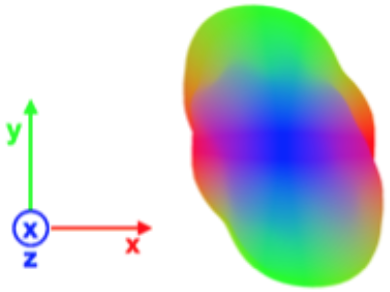
\includegraphics[width=.30\linewidth, angle=0]{figs/HARDI/ODF_normalizacao/ODF-pura.png}
    \label{fig::odf_pura}
    }
    \hspace{1em}
    \subfloat[ODF min-max normalizada] {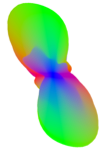
\includegraphics[width=.17\linewidth, angle=0]{figs/HARDI/ODF_normalizacao/ODF_minmax.png}
    \label{fig::odf_minmax}
    }
     \caption{Glifo ODF da mesma ODF com e sem a normalização min-max. A disposição de cores glifo enfatiza a orientação da ODF, no qual a direção dos eixos x, y, z estão mapeadas nas cores vermelha, verde e azul. Note que em \ref{fig::odf_minmax}, a estrutura orientacional da ODF é enfatizada com uma forte componente na direção do eixo y. O Capítulo \ref{chap::renderizacao_interativa_de_perfis_de_difusao} traz a formulação com detalhes do glifo.}
    \label{fig::normalizacao_min_max}
\end{figure}

\subsubsection{Domínio de amostragem}
%\subsection{Domínio esférico}
\label{ssec::dominio_esferico}

Tipicamente, as $S$ direções espaçadas para amostragem de ODFs,
$\mathbf{U} = [$
$\mathbf{\hat{u}}_1$, 
$\mathbf{\hat{u}}_2$, 
$\mathbf{\hat{u}}_3$, ..., 
$\mathbf{\hat{u}}_S$ 
$]$, são obtidas através de subdivisões de um icosaedro (Fig. \ref{fig::icosaedro}), como ilustra a Fig. \ref{fig::direcoes}. Na área na comunidade de DWI com métodos de alta ordem, esta categoria de malha é amplamente utilizada \cite{yeh2010, TuchQBall2004, descoteaux2007} e, de forma genérica, apresenta propriedades certas propriedades desejáveis  \cite{popko2012}:

\begin{enumerate}
    \item Seus doze vértices são uniformemente distribuídos e estão contidos em uma esfera;
    \item Os triângulos que definem a sua face são equiláteros;
    \item Todos os seus vértices tem um uma antípoda;
    \item provê malhas esféricas cujos os pontos são \textit{quasi}-isotrópicos \cite{popko2012}.
\end{enumerate}

Das propriedades descritas, a \textit{quasi}-isotropia torna esta malha desejável para o cômputo de máximos locais e cômputo de distribuição de fibras subjacentes \cite{descoteaux2007} e o fato de cada um dos seus vértices possuírem sua respectiva antípodas, permite que nós possamos nos aproveitar da simetria de ODFs de difusão para armazená-la em um só valor para antípodas na memória

\begin{figure}[ht]
%\subfigcapskip = -5pt
    \centering
    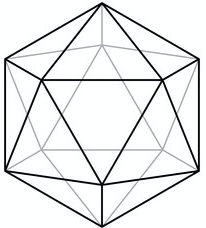
\includegraphics[width=.3\linewidth, angle=0]{figs/HARDI/icosaedro.png}
    \caption{
    Icosaedro.
    }
    \label{fig::icosaedro}
   \hspace{1pt}
\end{figure}

Há três procedimentos de subdivisões do icosaedro \cite{popko2012}: Subdivisão de classe I, classe II e classe III. Na classe I e II os \textit{grids} no triângulo do icosaedro são paralelos e perpendiculares às arestas, e na classe III, os \textit{grids} não apresentam esta restrição em relação às arestas. Fig. \ref{fig::classe_tesselacao} ilustra as categorias de subdivisão.

\begin{figure}[ht]
\centering
\captionsetup[subfloat]{farskip=0pt,nearskip=0pt}
\centering
    \subfloat[Classe I] {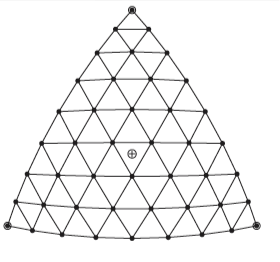
\includegraphics[width=.25\linewidth, angle=0]{figs/HARDI/Subdivisao_icosaedro/Classe_I.png}
    \label{fig::classe_i}
    }
    \hspace{1em}
    \subfloat[Classe II] {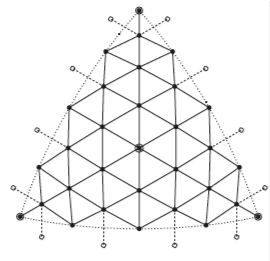
\includegraphics[width=.25\linewidth, angle=0]{figs/HARDI/Subdivisao_icosaedro/Classe_II.png}
    \label{fig::classe_ii}
    }
    \hspace{1em}
    \subfloat[Classe III] {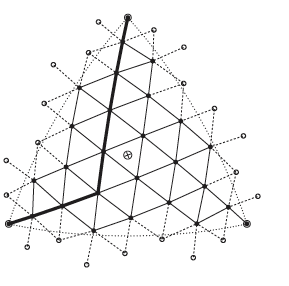
\includegraphics[width=.25\linewidth, angle=0]{figs/HARDI/Subdivisao_icosaedro/Classe_III.png}
    \label{fig::classe_iii}
    }
    \caption{Categorias de Tesselação do Icosaedro. Os vértices do icosaedro estão nas extremidades de cada malha, nas quais geram as subdivisões. Os pontos adicionados consistem nas intersecções dos \textit{grids} e são projetados na esfera.}
    \label{fig::classe_tesselacao}
\end{figure}

Destas classes, escolhemos a subdivisão de classe I. Ao contrário da classe III, as classe I e II garantem que os vértices adicionados na subdivisão tenham suas antípodas \cite{popko2012}. Adicionalmente, algoritmos para cômputo de vértices pela classe I e arestas da subdivisão são facilmente encontrados \cite{luna2012}.

A exemplificação mais simples do processo de subdivisão do icosaedro está ilustrado na Fig. \ref{fig::icosaedro_subdivisao}, na sua subdivisão em dois. O icosaedro está centrado em $(0,0,0)$ em cor vermelha. Cada aresta é dividida em duas partes iguais, no qual a mediana dos pontos conectados são adicionados. Em cada mediana de cada aresta do icosaedro, é definido um par de \textit{grids}. Cada um dos \textit{grids} 
é paralelo a uma das duas arestas do triângulo. O cômputo dos pontos de intersecções dos \textit{grids}. Os pontos computados são projetados na esfera, e novas arestas são adicionadas à malha e são referentes aos pontos que eram conectados pelos \textit{grid} antes da projeção (Fig. \ref{fig::icosaedro_normalizada}).

\begin{figure}[ht]
\centering
\captionsetup[subfloat]{farskip=0pt,nearskip=0pt}
\centering
    \subfloat[Novos vértices computados através das medianas do icosaedro] {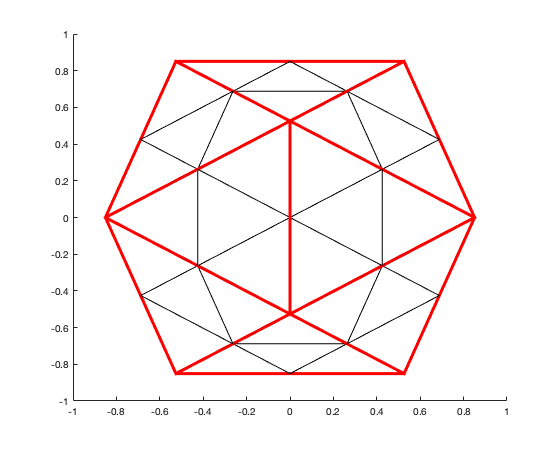
\includegraphics[width=.45\linewidth, angle=0]{figs/HARDI/Subdivisao_icosaedro/divisao_faces.png}
    \label{fig::icosaedro_faces}
    }
    \hspace{1em}
    \subfloat[Novos vértices projetados na esfera.] {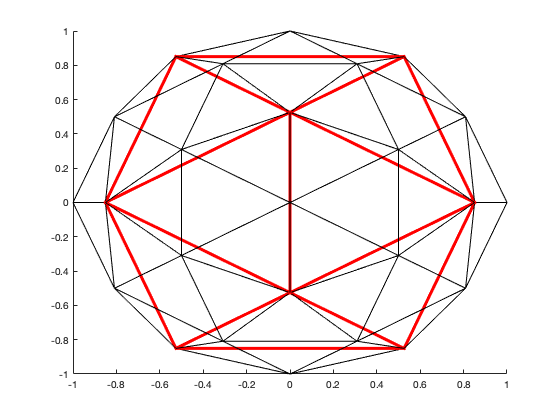
\includegraphics[width=.45\linewidth, angle=0]{figs/HARDI/Subdivisao_icosaedro/divisao_normalizada.png}
    \label{fig::icosaedro_normalizada}
    }
     \caption{Processo de subdivisão do icosaedro. As arestas são divididas em dois pontos iguais}
    \label{fig::icosaedro_subdivisao}
\end{figure}

Um exemplo análogo ao da Fig. \ref{fig::icosaedro_subdivisao}, que apresenta uma maior complexidade está na Fig. \ref{fig::icosaedro_subdivisao_4}, onde dividimos cada aresta do icosaedro em quatro segmentos, no qual adicionamos três pontos por aresta no processo de subdivisão. Definimos um par de \textit{grids} dentro para cada ponto adicionado, paralelos as outras duas arestas do seu respectivo triângulo, e computamos a intersecção de cada par de \textit{grids}. Todos os pontos computados na subdivisão dos segmentos no icosaedro e todas as intersecções dos \textit{grids} são projetadas na esfera (Fig. \ref{fig::icosaedro_normalizada_4}) e as novas arestas ligam os pontos que era conectados pelos \textit{grids} antes da projeção na esfera.

\begin{figure}[ht]
\centering
\captionsetup[subfloat]{farskip=0pt,nearskip=0pt}
\centering
    \subfloat[Novos vértices computados através das medianas do icosaedro] {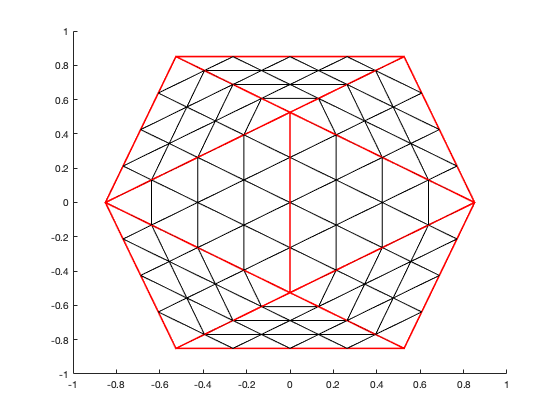
\includegraphics[width=.45\linewidth, angle=0]{figs/HARDI/Subdivisao_icosaedro/divisao_faces_4.png}
    \label{fig::icosaedro_faces_4}
    }
    \hspace{1em}
    \subfloat[Novos vértices projetados na esfera.] {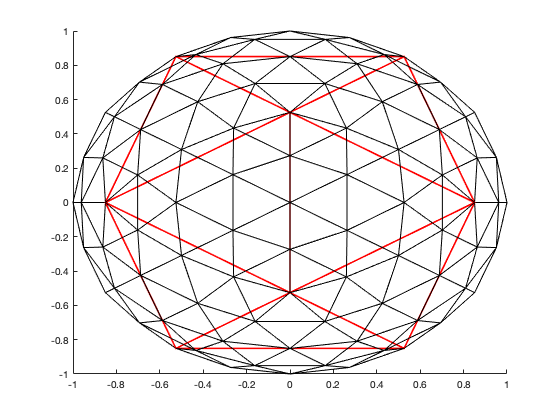
\includegraphics[width=.45\linewidth, angle=0]{figs/HARDI/Subdivisao_icosaedro/divisao_normalizada_4.png}
    \label{fig::icosaedro_normalizada_4}
    }
     \caption{Processo de subdivisão do icosaedro.}
    \label{fig::icosaedro_subdivisao_4}
\end{figure}

Observe que a projeção dos pontos intermediários adicionados na esfera subdivide cada aresta em dois e quatro, no exemplo ilustrados em Fig. \ref{fig::icosaedro_subdivisao} e \ref{fig::icosaedro_subdivisao_4}. Portanto, podemos referenciar esta categoria de subdivisão, que é classe I, na qual todas as arestas são divididas em $t$ segmentos de reta, pelo parâmetro $t$, no qual podemos inferir a quantidade de vértices e faces, representados nas Eq. \ref{eq::icosa_samples} e \ref{eq::icosphere_triangulos}, respectivamente \cite{popko2012}.

\begin{equation}
\label{eq::icosa_samples}
    N = 10\times t^2 + 2
\end{equation}

\begin{equation}
\label{eq::icosphere_triangulos}
\tau = 20\times t^2
\end{equation}

Podemos generalizar este procedimento de subdivisão para um parâmetro $t$, que representa as subdivisões de cada aresta para o seguinte procedimento:

\begin{enumerate}
    \item Subdividir cada aresta do icosaedro em $t$ segmentos iguais, onde os $t-1$ pontos da subdivisão terão suas projeções na esfera serão adicionados à malha;
    \item Para cada ponto nas arestas em cada triângulo, definir um par de \textit{grids} paralelos às outras arestas;
    \item computar as interseções de cada par de \textit{grids}, cujas projeções na esfera serão adicionadas à malha;
    \item computar as projeções na esfera de todos os novos pontos computados no passo (1) e (3).
\end{enumerate}

Nesta dissertação, referenciamos o processo descrito de subdivisão do icosaedro pelo parâmetro $t$ como a \textsf{$t$-ésima ordem de tesselação do icosaedro} ou \textsf{subdivisão de ordem $t$ do icosaedro}.

Neste trabalho, restringimo-nos a categoria de malhas feitas através das subdivisões de ordem $2^k$ do icosaedro. Além de todos os vértices da malha possuírem suas antípodas, esta categoria de malha apresenta mais uma característica desejável: há uma regularidade das facetas subdivididas, o que possibilita aumentar e diminuir a resolução dos glifos ODF de acordo com um modelo que relaciona sua ocupância na tela e resolução mantendo a qualidade da malha, conforme será detalhado no capítulo \ref{chap::renderizacao_interativa_de_perfis_de_difusao}. Algumas esferas aproximadas por tesselações uniformes do icosaedro estão ilustradas na Fig. \ref{fig::icosphere}. A quantidade de vértices para $2^a$, $4^a$, $8^a$ e $16^a$ ordem de tesselação é 42, 162, 642 e 2562, respectivamente.

\begin{figure}[ht]
\centering
\captionsetup[subfloat]{farskip=0pt,nearskip=0pt}
\centering
    \subfloat[Tesselação de $2^a$ ordem] {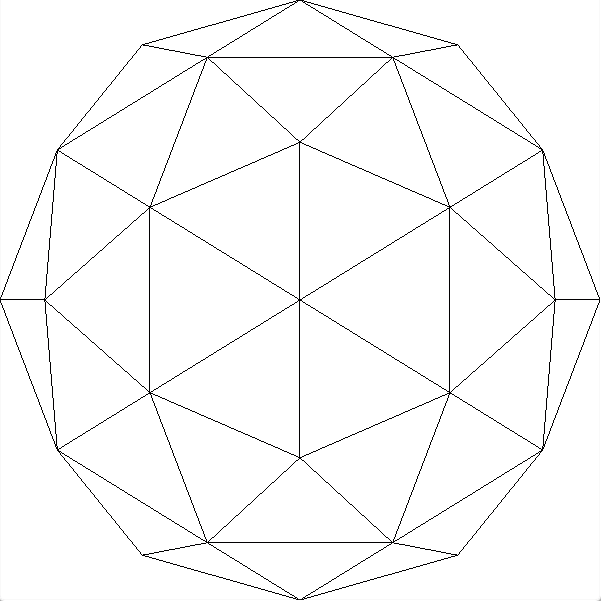
\includegraphics[width=.25\linewidth, angle=0]{figs/HARDI/Icosphere/icosphere_1.png}
    \label{fig::icosphere_1}
    }
    \hspace{1em}
    \subfloat[Tesselação de $4^a$ ordem] {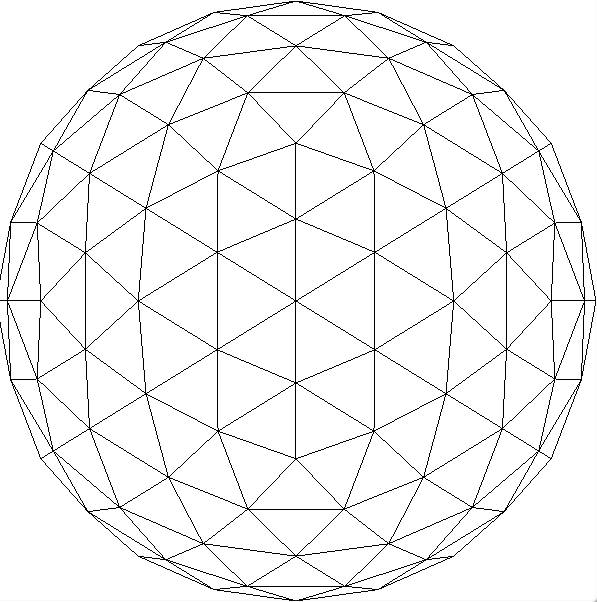
\includegraphics[width=.25\linewidth, angle=0]{figs/HARDI/Icosphere/icosphere_2.png}
    \label{fig::icosphere_2}
    }
    \\
    \subfloat[Tesselação de $8^a$ ordem] {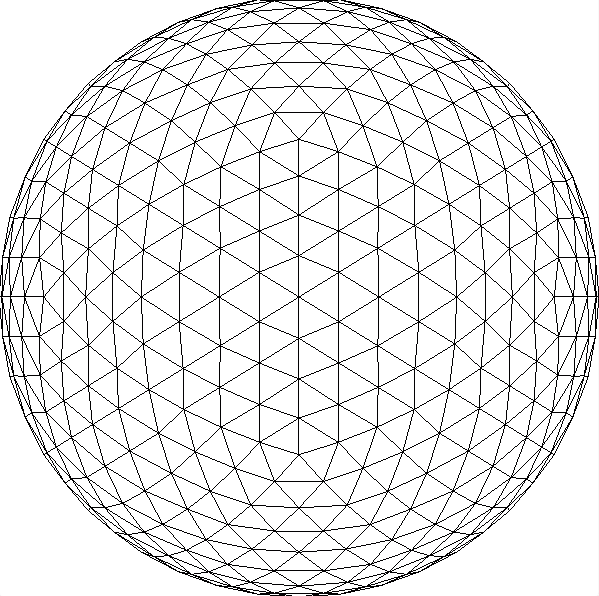
\includegraphics[width=.25\linewidth, angle=0]{figs/HARDI/Icosphere/icosphere_3.png}
    \label{fig::icosphere_3}
    }
    \hspace{1em}
    \subfloat[Tesselação de $16^a$ ordem]{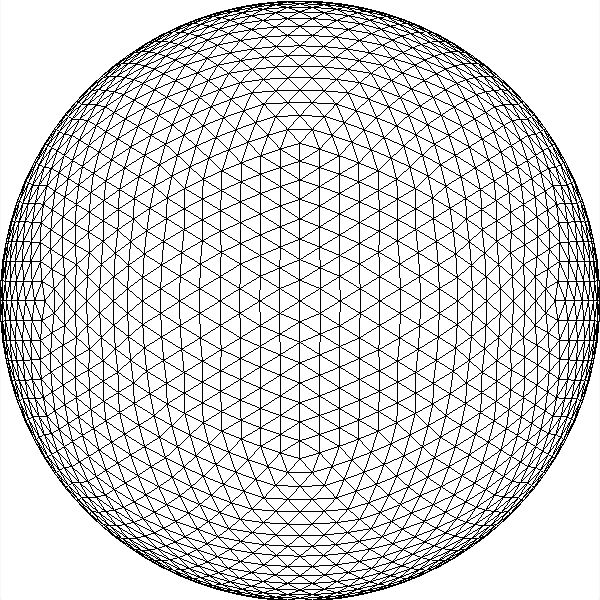
\includegraphics[width=.25\linewidth, angle=0]{figs/HARDI/Icosphere/icosphere_4.png}
    \label{fig::icosphere_4}
    }
     \caption{Esferas obtidas através da tesselação de um icosaedro.}
    \label{fig::icosphere}
\end{figure}


%através de \textit{grids}  divisão de cada aresta do icosaedro em N segmentos  corresponde à N-ésima ordem de tesselação do icosaedro 

%modalidade de subdivisão do icosaedro para geração da esfera para geração dos \textit{grids} pode ser referenciada pela quantidade de segmentos que dividimos cada aresta para gerar os grids



%para a classe de subdivisão escolhida, classificaremos a tesselação do icosaedro quanto a quantidade de pontos . 




\begin{figure}[ht]
%\subfigcapskip = -5pt
    \centering
    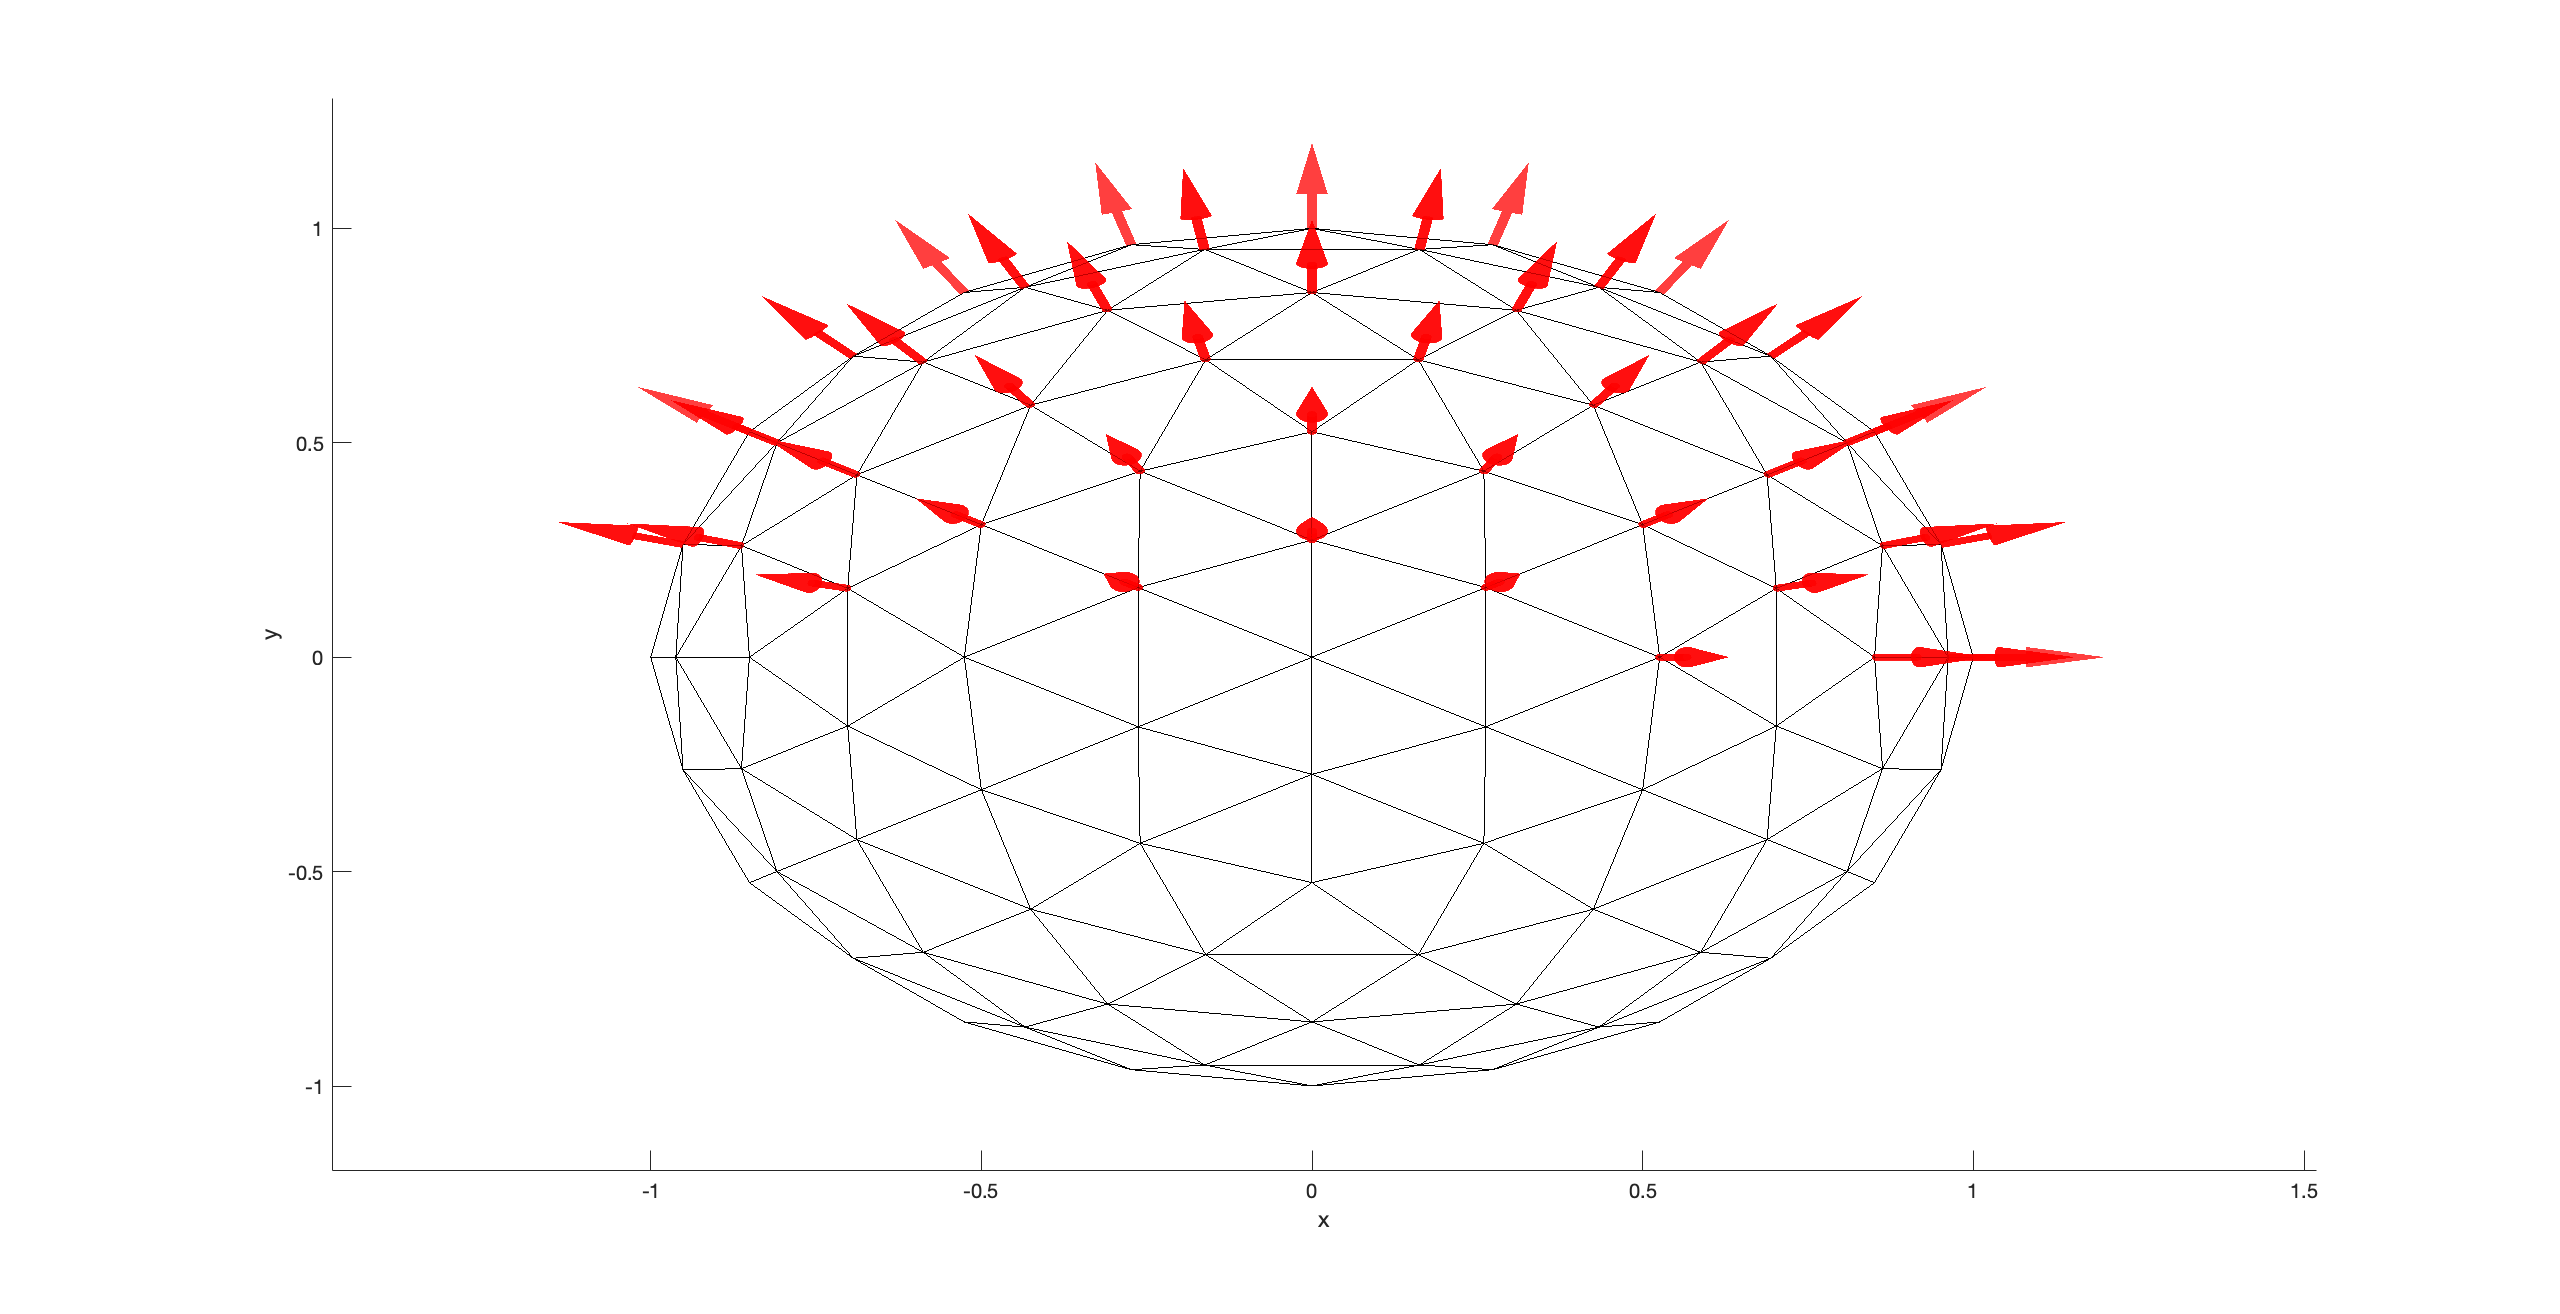
\includegraphics[width=.8\linewidth, angle=0]{figs/HARDI/icosphere_normals.png}
    \caption{
    Ilustração da extração do conjunto $\mathbf{U}$ da malha esférica obtida através da tesselação de $4^a$ ordem do icosaedro. Os vetores em vermelho indicam os vetores em $\mathbf{U}$ são extraídos dos pontos da esfera no hemisfério $x\geq 0$
    }
    \label{fig::direcoes}
   \hspace{1pt}
\end{figure}

\todo{\textcolor{green}{Direções amostradas com base em subdivisões de um icosaedro.}}


Para utilização mais eficiente do uso de memória, exploramos a simetria da ODF para definimos $\mathbf{U}$ para normais dos vértices da malha esférica dos pontos obtidos no hemisfério $y > 0 \cup (y = 0 \cap z > 0)$, conforme ilustrado em Fig. \ref{fig::direcoes}. Logo, para malha esférica escolhida com $N$ vértices, $\mathbf{U}_{3\times \frac{N}{2}} = [
\mathbf{n}_1,
\mathbf{n}_3, ..., 
\mathbf{n}_{N-3},
\mathbf{n}_{N-1}
]$. Nesta notação, indexamos os subíndices ímpares das normais $\mathbf{n}$ ao conjunto hemisfério.

Recomendamos que a ordem de tesselação para amostragem seja a oitava ou, no máximo, a décima sexta, implicando em 321 e 1281 amostras de ODF por \textit{voxel}. Valores acima destes computados para todo DWI pode incorrer no uso de uma quantidade proibitiva de memória.

\todo[inline]{Sugiro que sejam apresentados brevemente aqui diferentes procedimentos de subdivisão de icosaedros e destacar o procedimento de subdivisão uniforme. \textcolor{green}{FEITO!}}

A quantidade de amostras em função da ordem de tesselação do icosaedro é dada por:

onde $t$ é a ordem de tesselação. \textcolor{red}{.} \sout{A respeito das malhas esféricas mostradas na Fig. \ref{fig::icosphere}}, 




Neste trabalho, restringimo-nos a categoria de malhas feitas através das subdivisões de ordem $2^k$ do icosaedro. Esta categoria de malha apresenta duas características desejáveis: a primeira se refere a presença de pares simétricos em relação aos eixos coordenados (i.e., se o ponto $P$ está na malha, $-P$ também está);\todo{Esta segunda característica vale para quaisquer subdivisões ...} a segunda se refere a \sout{possibilidade de tirar proveito da percepção visual na renderização de glifos ODF,}\textcolor{red}{regularidade das facetas subdivididas,} o que possibilita aumentar e diminuir a resolução dos glifos ODF de acordo com um modelo que relaciona sua ocupância na tela e resolução \textcolor{red}{mantendo a qualidade da malha}, conforme será detalhado no capítulo \ref{chap::renderizacao_interativa_de_perfis_de_difusao}.

%\sout{A quantidade de amostras em função da ordem de tesselação do icosaedro é dada por:}
%\begin{equation}
%\label{eq::icosa_samples}
%    N = 10\times t^2 + 2
%\end{equation}
\sout{onde $t$ é a ordem de tesselação. A respeito das malhas esféricas mostradas na Fig. \ref{fig::icosphere}, a quantidade de vértices para $2^a$, $4^a$, $8^a$ e $16^a$ ordem de tesselação é 42, 162, 642 e 2562, respectivamente.}

\todo[inline]{Eu passaria os seguintes parágrafos para um capítulo em que você apresenta a sua proposta.}
\textcolor{magenta}{
Seja o conjunto $\Pi = \{P_1, P_2, \dots, P_N\}$\footnote{Na Seção \ref{ssec::geometria_base} do Capítulo \ref{chap::renderizacao_interativa_de_perfis_de_difusao}, sugerimos diretrizes para a formulação da estrutura de dados dos pontos de $\Pi$.} o conjunto de vértices da malha esférica obtida através da subdivisão do icosaedro. Para que possamos tomar vantagem da simetria de ODFs, condicionamos que $P_{2K+2} = -P_{2K+1}$ $(0 \leq K \leq \frac{N-2}{2})$.
}
\textcolor{magenta}{
Pode-se atribuir ao vetor $\mathbf{U} = [
\mathbf{n}_1, 
\mathbf{n}_2, ...,
\mathbf{n}_{N-1},
\mathbf{n}_N
]$, nos quais cada $\mathbf{n}_i$ é o vetor unitário na direção e sentido do vetor normal de $P_i$ ($P_i \in \Pi$), no entanto podemos tirar vantagem da simetria da ODF e reduzir o seu tamanho pela metade. Os pontos simétricos em relação aos eixos da esfera tem normais em sentidos opostos, ou seja, $\mathbf{n}_{2K+2} = -\mathbf{n}_{2K+1}$, $(0 \leq K \leq \frac{N-2}{2})$. Observe que a função $\psi_m(\mathbf{r}, \mathbf{\hat{u}})$ (Eq. \ref{eq::sdf_discrete_2}) é simétrica em relação aos eixos em $\mathbf{\hat{u}}$, $\psi_m(\mathbf{r}, \mathbf{\hat{u}}) = \psi_m(\mathbf{r}, \mathbf{-\hat{u}})$, implicando que $\psi_m(\mathbf{r}, \mathbf{n}_{2K+2}) = \psi_m(\mathbf{r}, \mathbf{n}_{2K+1})$.
}
\textcolor{magenta}{
Assim, para utilização mais eficiente do uso de memória, definimos $\mathbf{U}$ para normais dos vértices da malha esférica, mapeando o par de normais de sentidos opostos em uma única direção. Logo $\mathbf{U}_{3\times \frac{N}{2}} = [
\mathbf{n}_1,
\mathbf{n}_3, ..., 
\mathbf{n}_{N-3},
\mathbf{n}_{N-1}
]$, onde o vetor na K-ésima  posição de $\mathbf{U}$ é $\mathbf{\hat{n}}_{2K-1}$. Observe que após o cômputo, $\boldsymbol{\psi}(\mathbf{r})$ tem na K-ésima posição os valores de ODF associadas à $\mathbf{n}_{2K-1}$, e também a direção $\mathbf{n}_{2K}$.
}
\textcolor{magenta}{
Recomendamos que a ordem de tesselação para amostragem seja a oitava ou, no máximo, a décima sexta, implicando em 321 e 1281 amostras de ODF por \textit{voxel}. Valores acima destes computados para todo DWI pode incorrer no uso de uma quantidade proibitiva de memória.
}



%Pode-se estabelecer que a estrutura de dados de $\mathbf{U}$ seja $[\mathbf{u_1}, \mathbf{u_2}, ..., \mathbf{u_{N-1}}, \mathbf{u_{N}}]^T$. Porém, podemos aproveitar a simetria dos dados e da malha esférica utilizada e organizarmos os dados de tal forma que um valor de ODF guardado na memória seja associado a duas direções simétricas.

\section{Visualização de Direções Intravoxeis}

\todo[inline]{Sugiro abrir uma seção e que você mostra visualização de potencias direções intravoxeis.}

\textcolor{red}{Embora as ODFs proveem informações mais precisas sobre as direções de potenciais fibras que cruzam um \textit{voxel}, a grande quantidade de dados numéricos envolvidos em ODFs de um volume de ressonância magnética ponderada por difusão torna difícil avaliar a plausibilidade das amostras adquiridas em relação à anatomia da substância branca cerebral e aplicá-las para provas de conceito de esquemas de aquisição de tensores de alta ordem. A forma mais comum de superar esta dificuldade é visualizar os dados numéricos das ODFs em glifos provenientes da superfície definida pela plotagem polar esférica $R(\mathbf{\hat{u}})$. Estes glifos permitem sintetizar numa única imagem não só o comportamento local (intravoxel) de difusão como também as relações intervoxeis.} 

\subsection{Glifos ODF}
\label{sec::glifos_odf}

%Como descrito na seção \ref{sec::trabalhos_relacionados_glifos}
\subsubsection{Superfície}

A superfície do glifo da ODF no voxel de coordenadas $\mathbf{r}$ $\psi(\mathbf{r}, \mathbf{\hat{u}})$ consiste na plotagem polar esférica onde $R(\mathbf{\hat{u}}) = \psi(\mathbf{r}, \mathbf{\hat{u}})$. A plotagem polar esférica $R(\mathbf{\hat{u}})$ é uma superfície na qual a distância da origem para um dos seus respectivos pontos na direção $\mathbf{\hat{u}}$ é dado por $R(\mathbf{\hat{u}})$.

% é dada por  na modulação do raio na direção $\mathbf{u}$ de uma esférica de acordo com uma versão normalizada do seu valor de imagem na função $\psi(\mathbf{u})$. A normalização que fizemos neste trabalho para representação está representado na equação \ref{eq::normglifo2}.

%\begin{equation}
%\label{eq::normglifo2}
%    R(\mathbf{u}) = \frac{\psi(\mathbf{u}) - min(\psi(\mathbf{u}))}{max(\psi(\mathbf{u})) - min(\psi(\mathbf{u}))}
%\end{equation}
\subsubsection{Cor}

As componentes r, g e b do mapeamento de cor esférica do glifo é dado em função da direção $\mathbf{\hat{u}} = (u_x, u_y, u_z)$, como definido em Eq. \ref{eq::cor_glifo} e ilustrado nos glifos da Fig. \ref{fig::glifo_ilustrado}. Esta forma de mapear, além de simples, é comumente utilizado pela comunidade DWI. %\todo{É imprescincível adicionar esta informação?}\sout{Não foi implementado o cômputo de vetores normais à superfície representadas pelo glifo, que consequentemente não tem iluminação associada.}

\begin{equation}
\label{eq::cor_glifo}
    r = |u_x| ~~~~ g = |u_y| ~~~~ b = |u_z|, 
\end{equation}

\begin{figure}[ht]

%\subfigcapskip = -5pt
    \centering
    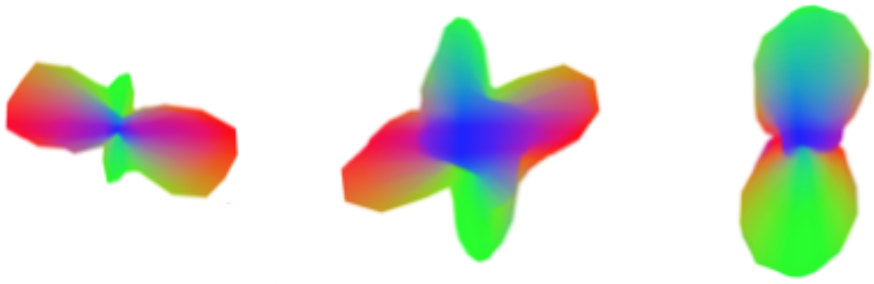
\includegraphics[width=.8\linewidth, angle=0]{figs/Esquema_Glifo/Glifos3Ex.png}
    \caption{Exemplos de glifos ODF. Os glifos consistem em uma superfície plotagem polar com a cor esquematizada de acordo com a equação \ref{eq::cor_glifo}.}
    \label{fig::glifo_ilustrado}
   \hspace{1pt}
\end{figure}

A respeito de planos anatômicos, a cor vermelha (r) representa a direção mediolateral, a verde (g), se refere a direção anteroposterior, e a azul (b), a direção inferior-superior.

\subsubsection{Realce}

Com o objetivo de enfatizar as direções dominantes de difusão na renderização de glifos, \citeonline{TuchQBall2004} sugere normalizar cada função de distribuição de \textit{spins} $\boldsymbol{\psi}_m(\mathbf{r})$ pela normalização min-max, \textcolor{red}{cujo resultado Sicrano \cite{???} mostrou que é uma} ODF $\boldsymbol{\psi}(\mathbf{r})$\sout{, conforme mostrado na Eq. \ref{eq::SDF2dODF}.} 

\begin{equation}
\label{eq::SDF2dODF}
    \boldsymbol{\psi}(\mathbf{r}) = [ \frac{\boldsymbol{\psi}_m(\mathbf{r}) - \text{min}(\boldsymbol{\psi}_m(\mathbf{r}))}{\text{max}(\boldsymbol{\psi}_m(\mathbf{r})) - \text{min}(\boldsymbol{\psi}_m(\mathbf{r}))}], m = 1, \cdots, S ,
\end{equation}
onde $\text{min}(\boldsymbol{\psi}_m(\mathbf{r}))$ e $\text{max}(\boldsymbol{\psi}_m(\mathbf{r}))$ são, respectivamente, o mínimo e o máximo dos $S$ valores associados à amostra $\mathbf{r}$.

O efeito da normalização está ilustrado na Fig. \ref{fig::normalizacao_min_max}. Observe que a normalização cancela o fator de escala $A_qL_{\Delta}$ da Eq. \ref{eq::s_ij}.

%\begin{equation}
%\label{eq::SDF2dODF}
%    \boldsymbol{\psi}(\mathbf{r}) = [ \frac{\boldsymbol{\psi}_m(\mathbf{r}) - %\text{min}(\boldsymbol{\psi}_m(\mathbf{r}))}{\text{max}(\boldsymbol{\psi}_m(\mathbf{r})) - %\text{min}(\boldsymbol{\psi}_m(\mathbf{r}))}], m = 1, \cdots, S
%\end{equation}

\begin{figure}[ht]
\centering
\captionsetup[subfloat]{farskip=0pt,nearskip=0pt}
\centering
    \subfloat[ODF não normalizada] {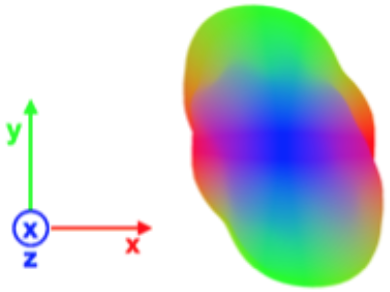
\includegraphics[width=.30\linewidth, angle=0]{figs/HARDI/ODF_normalizacao/ODF-pura.png}
    \label{fig::odf_pura}
    }
    \hspace{1em}
    \subfloat[ODF min-max normalizada] {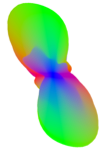
\includegraphics[width=.17\linewidth, angle=0]{figs/HARDI/ODF_normalizacao/ODF_minmax.png}
    \label{fig::odf_minmax}
    }
     \caption{Glifo ODF da mesma ODF com e sem a normalização min-max. A disposição de cores glifo enfatiza a orientação da ODF, no qual a direção dos eixos x, y, z estão mapeadas nas cores vermelha, verde e azul. Note que em \ref{fig::odf_minmax}, a estrutura orientacional da ODF é enfatizada com uma forte componente na direção do eixo y. O Capítulo \ref{chap::renderizacao_interativa_de_perfis_de_difusao} traz a formulação com detalhes do glifo.}
    \label{fig::normalizacao_min_max}
\end{figure}


\chapter{Renderização interativa de perfis de difusão}
\label{chap::renderizacao_interativa_de_perfis_de_difusao}

\todo[inline]{Perfis de difusão? Ou ODFs? Vamos evitar uso de termos distintos para referenciar um mesmo objeto?}

%\todo[inline]{Falta contextualizar nos objetivos que você listou na seção 1.3. Não é melhor focar em renderização de perfis de difusão que é um dos problemas relacionados diretamente com a interatividade?}

A forma mais comum de visualizar dados derivados de ODFs é através glifos provenientes da superfície definida pela plotagem polar esférica $R(\mathbf{\hat{u}})$. Esta classe de superfície permite a inferência e inspeção de ODFs de difusão e sua distribuição de fibras subjacentes. Adicionalmente, permite a avaliação visual das ODFs obtidas a partir de um método HARDI para diferentes aquisições. Estes glifos dão uma visualização clara do comportamento local de difusão e são amplamente utilizados para provas de conceito em trabalhos na área de HARDI e essenciais para visualização dos resultados gerados pelos métodos de alta ordem.

\sout{Alguns dos exemplos de}\textcolor{red}{Entre os} trabalhos que \textcolor{red}{utilizam} os \textcolor{red}{glifos}\sout{utilizam}, temos\sout{:} \citeonline{TuchQBall2004},  \citeonline{yeh2010},  \citeonline{daducci2014}  e  \citeonline{descoteaux2007}. \citeonline{TuchQBall2004},  \citeonline{yeh2010} os utilizam como ferramenta de visualização para o\textcolor{red}{s} método\textcolor{red}{s} de imageamento propostos em seus respectivos trabalhos. \citeonline{daducci2014} os utiliza para ilustrar e comparar ODFs reconstruídas por diferentes métodos. E \citeonline{descoteaux2007} \textcolor{red}{aplicam os glifos}  para ilustrar transformações entre ODFs \todo{Não entendi nos seus respectivos algoritmos de tractografia!}\textcolor{magenta}{nos seus respectivos algoritmos de tractografia propostos}. \todo{Não entendi a observação. GQI foi uma técnica que você escolheu para gerar ODFs ... Em tese, ODFs podem ser geradas por outras técnicas.}\sout{Isto evidencia que o algoritmo de renderização que estamos propondo não é restrito somente ao método GQI que apresentamos no Capítulo \ref{chapter::metodos_hardi}.}
\textcolor{red}{Além de proporcionar melhor entendimento dos dados adquiridos pelas técnicas de alta ordem, conjeturamos que a visualização das ODFs através de glifos posicionados em seus respectivos \textit{voxels} sobrepostos a um volume de ressonância magnética ponderada em T1 pode melhorar o processo de escolha de sementes para tractografias baseadas em sementes. \citeonline{voltoline2021} trazem algumas evidências das circunstâncias em que os superquádricos do DTI podem melhorar este processo.}

\todo[inline]{Sugiro que você expanda o seguinte parágrafo tocando brevemente (1) o foco desta dissertação (visualização interativa de ODFs $\rightarrow$ renderização de ODFs em tempo interativo em GPU); (2) potenciais problemas (tráfego CPU-GPU, limitada memória da GPU, otimização na renderização) $\rightarrow$ mapeamento de ODFs em modelos geométricos, redução de tráfego, ocupação da memória de GPU;  e (3) o estado-da-arte.}

\textcolor{magenta}{
Neste capítulo, apresentamos o algoritmo de renderização interativa de ODFs através de glifos, integrado ao ambiente de visualização multimodal para visualização DWI. Mostraremos como resultados aspectos visuais e sua performance, na qual atestamos a sua interatividade.
}

\textcolor{magenta}{O capítulo está organizado em 5 seções. Na Seção \ref{sec::glifos_odf} descreveremos a superfície e cor dos glifos, no qual chamaremos de glifos ODF; na Seção \ref{sec::trabalhos_relacionados}, apresentamos os trabalhos relacionados; na Seção \ref{sec::superquadricas}, apresentamos brevemente a \textit{pipeline} de renderização multimodal para superquádricos proposto por \citeonline{voltoline2021}; na Seção \ref{sec::renderizacao_de_glifos_ODF}, apresentamos a modificação na \textit{pipeline} da renderização multimodal para superquádricas e a nossa abordagem para renderização de glifos ODF; na Seção \ref{sec::experimentos}, mostramos a performance do esquema de renderização e aspectos visuais.
}
\textcolor{magenta}{
Na Subseção \ref{ssec::aspectos_visuais}, mostramos que esses glifos são mais informativos que os superquádricos por permitir o inferimento do cruzamento de fibras.
}

\sout{Este algoritmo de renderização, integrado a um sistema de visualização para DWI pode ser uma ferramenta poderosa para pesquisadores da área para avaliar perfis de difusão locais e melhorar o seu entendimento em métodos de alta ordem.
Adicionalmente, temos a conjectura que as ODFs representadas através de glifos posicionados em seus respectivos \textit{voxels} no ambiente de visualização multimodal pode melhorar o processo de escolha de parâmetros iniciais em tractografia. \citeonline{voltoline2021} trazem algumas evidências das circunstâncias que os superquádricos do DTI podem melhorar este processo, e conforme mostramos na Subseção \ref{ssec::aspectos_visuais}, mostramos que esses glifos são mais informativos que os superquádricos por permitir o inferimento do cruzamento de fibras.
}

\sout{O capítulo está organizado em 5 seções. Na Seção \ref{sec::glifos_odf} descreveremos a superfície e cor dos glifos, no qual chamaremos de glifos ODF; na Seção \ref{sec::trabalhos_relacionados}, apresentamos os trabalhos relacionados; na Seção \ref{sec::superquadricas}, apresentamos brevemente a \textit{pipeline} de renderização multimodal para superquádricos proposto por \citeonline{voltoline2021}; na Seção \ref{sec::renderizacao_de_glifos_ODF}, apresentamos a modificação na \textit{pipeline} da renderização multimodal para superquádricas e a nossa abordagem para renderização de glifos ODF; na Seção \ref{sec::experimentos}, mostramos a performance do esquema de renderização e aspectos visuais.}


%\todo[inline]{Eu deixaria o parágrafo abaixo para conclusões}

\section{Trabalhos Relacionados}
\label{sec::trabalhos_relacionados}

Apesar da relevância reconhecida da renderização interativa de dados de ODF, a comunidade não tem explorado muito esta questão. \sout{Por questões de performance}\textcolor{red}{Para poder atender ao requisito de interatividade}, \sout{nos limitaremos}\textcolor{red}{limitáremo-nos} a trabalhos que exploram recursos da GPU. Há duas grandes abordagens \sout{achadas na literatura} para renderização de glifos. A primeira é baseada em \textit{ray-casting}, onde a geometria do glifo é representada por uma função ou expressão algébrica \cite{peeters2009, almsick2011}. A outra é baseada na renderização de malhas, com a geometria do glifo aproximada por malhas poligonais \cite{shattuck2008}.

\todo[inline]{Sendo uma dissertação, você deve discutir melhor as técnicas apresentadas em relação à solução dada à lista dos potenciais problemas.}

\citeonline{shattuck2008} tessela uma representação polar de ODF com triângulos, onde a superfície do glifo é gerada através da discretização do seu domínio polar, e sua forma é gerada na CPU através de uma função analítica neste domínio. Os glifos são renderizados por fatia. Com a mudança de malha e parâmetros de visualização, os vertices do glifo são re-computados e reenviados à GPU. A performance relatada é de dez \textit{frames}/s para uma fatia de um volume, no qual cada glifo tem 225 vértices, em uma cena com aproximadamente 2 milhões de triângulos. Neste trabalho, exploramos recursos da GPU modernos para melhorar a performance de renderização e seu uso de memória.


\citeonline{peeters2009} apresentaram um esquema de renderização utilizando \textit{ray-casting}. Na CPU, o centro, o raio da esfera delimitadora e o cubo delimitador por glifo são computados. Na GPU, o algoritmo de ray-casting é executdo por pixel no \textit{fragment shader}. Se o raio lançado para um pixel não intercepta a esfera delimitadora, o fragmento é descartado. Caso contrário, o algoritmo executa uma busca linear ,com passos discretos para interseção da ODF para com o raio. Eles alcançaram uma melhor performance que o algoritmo apresentado por \citeonline{shattuck2008}. \citeonline{almsick2011} melhorou a busca por interseção utilizando o método numérico \textit{regula falsi} e cilindros delimitadores alinhados com o eixo de visão. Eles atingiram um melhor tempo de performance sem sacrificar a qualidade de renderização, documentando que 9000 glifos puderam ser gerados a 30 FPS. Há um problema crítico na acurácia e eficiência do raio lançado. Quando o raio tende a ser paralelo ao glifo, muitas iterações podem ocorrer em algumas \textit{threads}. A renderização baseada em triângulos que propomos neste trabalho não apresenta este problema. 

\citeonline{voltoline2021} propuseram um esquema de renderização para glifos superquádricos para tensores de difusão \cite{Kindlmann2004}. Eles exploraram recursos modernos da GPU para atingir este objetivo, que consistem em \textit{transform feedback}, aproximação triangular adaptativa dos glifos e renderização por instanciação indireta. Diferentemente das superquádricas, os dados associados com glifos ODF tem dimensionalidade bem maior, o que inviabiliza seu armazenamento na GPU. Consequentemente, devemos propor estratégias para minimizar o tráfego de dados CPU-GPU para os glifos a serem renderizados, almejando a interatividade.



%Esta classe de glifos são amplamente utilizados como uma ferramenta de visualização para prova de conceito em trabalhos na área de DWI. Além de \citeonline{TuchQBall2004}, alguns trabalhos relacionadosque os utilizam são: \citeonline{SCHILLING2019194}, para ilustrar a eficácia de métodos HARDI na detecção de direções de difusão, \citeonline{descoteaux2007}, para ilustrar o efeito de um\sout{a técnica} \todo{qual pré-processamento?}pré-processamento \sout{proposto} em ODFs que melhora a tractografia e \citeonline{yeh2010} 

%Foi implementado um esquema de visualização para ODFs em glifos de acordo através de representações gráficas polares esféricas. A implementação serviu primeiramente para prova de conceito e posteriormente otimizada para que seja possível a sua renderização, \textit{voxel} a \textit{voxel}, em tempo interativo pelo VMTK-Neuro, o que foi possível nos testes feitos em um Macbook Pro Retina 13', com processador Intel Core i5 Dual-Core 2.7Ghz, processador gráfico Intel Iris Graphics 6100 1536 MB e memória RAM de 8 GB 1867 MHz DDR3.

%\todo[inline]{Fazer uma breve justificativa da relevância da visualização das ODFs no contexto da sua proposta de uma visualização interativa almejando uma tractografia mais próxima dos tratos reais.}

\section{Glifos ODF}
\label{sec::glifos_odf}

%Como descrito na seção \ref{sec::trabalhos_relacionados_glifos}
\subsection{Superfície}

A superfície do glifo da ODF no voxel de coordenadas $\mathbf{r}$ $\psi(\mathbf{r}, \mathbf{\hat{u}})$ consiste na plotagem polar esférica onde $R(\mathbf{\hat{u}}) = \psi(\mathbf{r}, \mathbf{\hat{u}})$. A plotagem polar esférica $R(\mathbf{\hat{u}})$ é uma superfície na qual a distância da origem para um dos seus respectivos pontos na direção $\mathbf{\hat{u}}$ é dado por $R(\mathbf{\hat{u}})$.

% é dada por  na modulação do raio na direção $\mathbf{u}$ de uma esférica de acordo com uma versão normalizada do seu valor de imagem na função $\psi(\mathbf{u})$. A normalização que fizemos neste trabalho para representação está representado na equação \ref{eq::normglifo2}.

%\begin{equation}
%\label{eq::normglifo2}
%    R(\mathbf{u}) = \frac{\psi(\mathbf{u}) - min(\psi(\mathbf{u}))}{max(\psi(\mathbf{u})) - min(\psi(\mathbf{u}))}
%\end{equation}
\subsection{Cor}

As componentes r, g e b do mapeamento de cor esférica do glifo é dado em função da direção $\mathbf{\hat{u}} = (u_x, u_y, u_z)$, como definido em Eq. \ref{eq::cor_glifo} e ilustrado nos glifos da Fig. \ref{fig::glifo_ilustrado}. Esta forma de mapear, além de simples, é comumente utilizado pela comunidade DWI. %\todo{É imprescincível adicionar esta informação?}\sout{Não foi implementado o cômputo de vetores normais à superfície representadas pelo glifo, que consequentemente não tem iluminação associada.}

\begin{equation}
\label{eq::cor_glifo}
    r = |u_x| ~~~~ g = |u_y| ~~~~ b = |u_z|, 
\end{equation}

\begin{figure}[ht]

%\subfigcapskip = -5pt
    \centering
    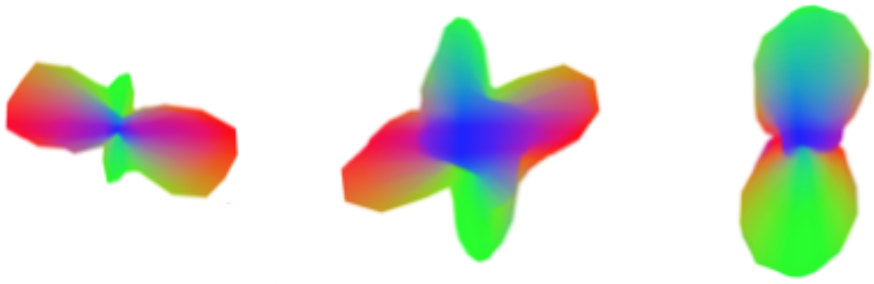
\includegraphics[width=.8\linewidth, angle=0]{figs/Esquema_Glifo/Glifos3Ex.png}
    \caption{Exemplos de glifos ODF. Os glifos consistem em uma superfície plotagem polar com a cor esquematizada de acordo com a equação \ref{eq::cor_glifo}.}
    \label{fig::glifo_ilustrado}
   \hspace{1pt}
\end{figure}

A respeito de planos anatômicos, a cor vermelha (r) representa a direção mediolateral, a verde (g), se refere a direção anteroposterior, e a azul (b), a direção inferior-superior.

\section{Renderização multimodal de glifos superquádricas}
\label{sec::superquadricas}

\citeonline{voltoline2021} propuseram um algoritmo de renderização multimodal de glifos superquádricos sobre o seu respectivo MRI anatômico ponderado em T1. O volume $b0$, seu respectivo MRI T1 e a matriz rígida que co-registra ambos os volumes \cite{ting2014} são enviadas à GPU.

O algoritmo de renderização é dividido em três estágios: (1) renderização do DWI e do volume anatômico; (2) detecção dos \textit{voxels} visíveis e estimativa da cobertura máxima da projeção dos glifos em \textit{pixels}, para estimativa da resolução da malha; (3) renderização de \textit{voxels} visíveis na resolução estimada.

Para manter a compatibilidade do algoritmo com o Mac OSX, cuja versão máxima suportada do OpenGL é 4.1, eles desdobraram o algoritmo para estimação de cobertura máxima de \textit{pixels} para os glifos de um passo, onde a implementação é feita no \textit{compute shader} em um algoritmo de quatro passos, envolvendo \textit{vertex, geometry} e \textit{fragment shaders} baseados em rasterização. Para evitar transferência de dados entre CPU e GPU entre passos, o \textit{transform feedback buffer} foi aplicado. Adicionalmente, eles mostraram a utilização do mecanismo de \textit{additive blending} para obtenção do número máximo de \textit{pixels} ($max_p$), no qual o \textit{voxel} é projetado em um volume \textit{ray-casted}. Baseado em $max_p$, eles estabelecem uma heurística para estimação da resolução da malha.

Através de $max_p$, um \textit{tessellation shader} é acionado para gerar o \textit{skeleton} base dos superquádricos, no qual eles utilizam o comando renderização indireta por instâncias para desenhá-los com uma chamada desenho. Provendo a parâmetros particulares a cada \textit{voxel} que definem cada superquádrico, em cada instância o \textit{skeleton} é customizado para gerar o glifo e é posicionado em seu respectivo \textit{voxel} no espaço do volume.


\section{Renderização de Glifos ODF}
\label{sec::renderizacao_de_glifos_ODF}

\textcolor{red}{Para renderizar os dados numéricos dos perfis de difusão em GPUs, é necessário mapear os dados em atributos de modelos geométricos processáveis pelas GPUs.} \todo{Nossa proposta? Ou já é uma ideia antiga? Cite uma referência.}\textcolor{magenta}{Em nossa abordagem}, o glifo é sintetizado pelo deslocamento dos $S$ pontos  \todo{Não ficaria melhor $S$, como no cap. 2?}$\{
P_1,
P_2, ...,
P_N
\}$
de uma malha esférica unitária base\textcolor{red}{, centrada em $\mathbf{r}$,} em função de \sout{$R(\mathbf{\hat{u}})$} \textcolor{red}{$\psi (\mathbf{r, \mathbf{n}_i}) \mathbf{n}_i$, onde $\mathbf{n}_i$ é o vetor normal à malha esférica no ponto $P_i$ e $\psi (\mathbf{r, \mathbf{n}_i})$ é a função de distribuição de \textit{spin} de orientação $\mathbf{n}_i$} . \sout{Para uma malha esférica cujo conjunto de vértices é dado por $\{
P_1,
P_2, ...,
P_S
\}$, o glifo de uma ODF $R(\mathbf{\hat{u}})$ é gerado pelo escalonamento de cada um dos pontos $P_K$ da malha $(1 \leq K \leq N)$ pelo seu respectivo $R(\mathbf{n_K})$, onde $\mathbf{n_K}$ é o vetor unitário com direção e sentido da normal do ponto na esfera em $P_K$.}


% A ODF associada a um \textit{voxel} é tipicamente representada por um conjunto de $N$ amostras de difusão $[
% R(\mathbf{\hat{n}}_1), 
% R(\mathbf{\hat{n}}_2), ...,
% R(\mathbf{\hat{n}}_{N-1}),
% R(\mathbf{\hat{n}}_N)
% ]^T$, onde cada $\mathbf{\hat{n}}_i$ é tem a direção e sentido da normal de cada ponto $ P_i$ de uma malha esférica. O glifo é sintetizado pelo deslocamento de cada ponto $P_i$ pelo seu escalar associado $R(\mathbf{\hat{n}}_i)$. Todas as amostras e ODF são computadas, conforme mostrado no Capítulo \ref{chapter::metodos_hardi} e acessíveis pelos seus respectivos ínndices de \textit{voxel}.


Devido a limitação de memória da GPU,  aplicamos o algoritmo de detecção de \textit{voxels} visíveis \cite{voltoline2021} para obtermos um conjunto de $D = [
\mathbf{d}_1,
\mathbf{d}_2, ..., 
\mathbf{d}_M
]$ \textit{voxels} visíveis e sugerimos o envio à GPU das suas respectivas ODFs para renderização por instância, como ilustrado na Fig. \ref{fig::vmtk_simplified}. Este procedimento causa uma penalidade em performance devido ao tráfego de dados CPU-GPU devido as mudanças frequentes nas imagens renderizadas em função da interação com o usuário. Assim, nesta seção, apresentamos estratégias para enfrentar esta transferência afim de obter a renderização de forma interativa.


\begin{figure}[ht]
    \centering
    %\rule{6cm}{3cm}
    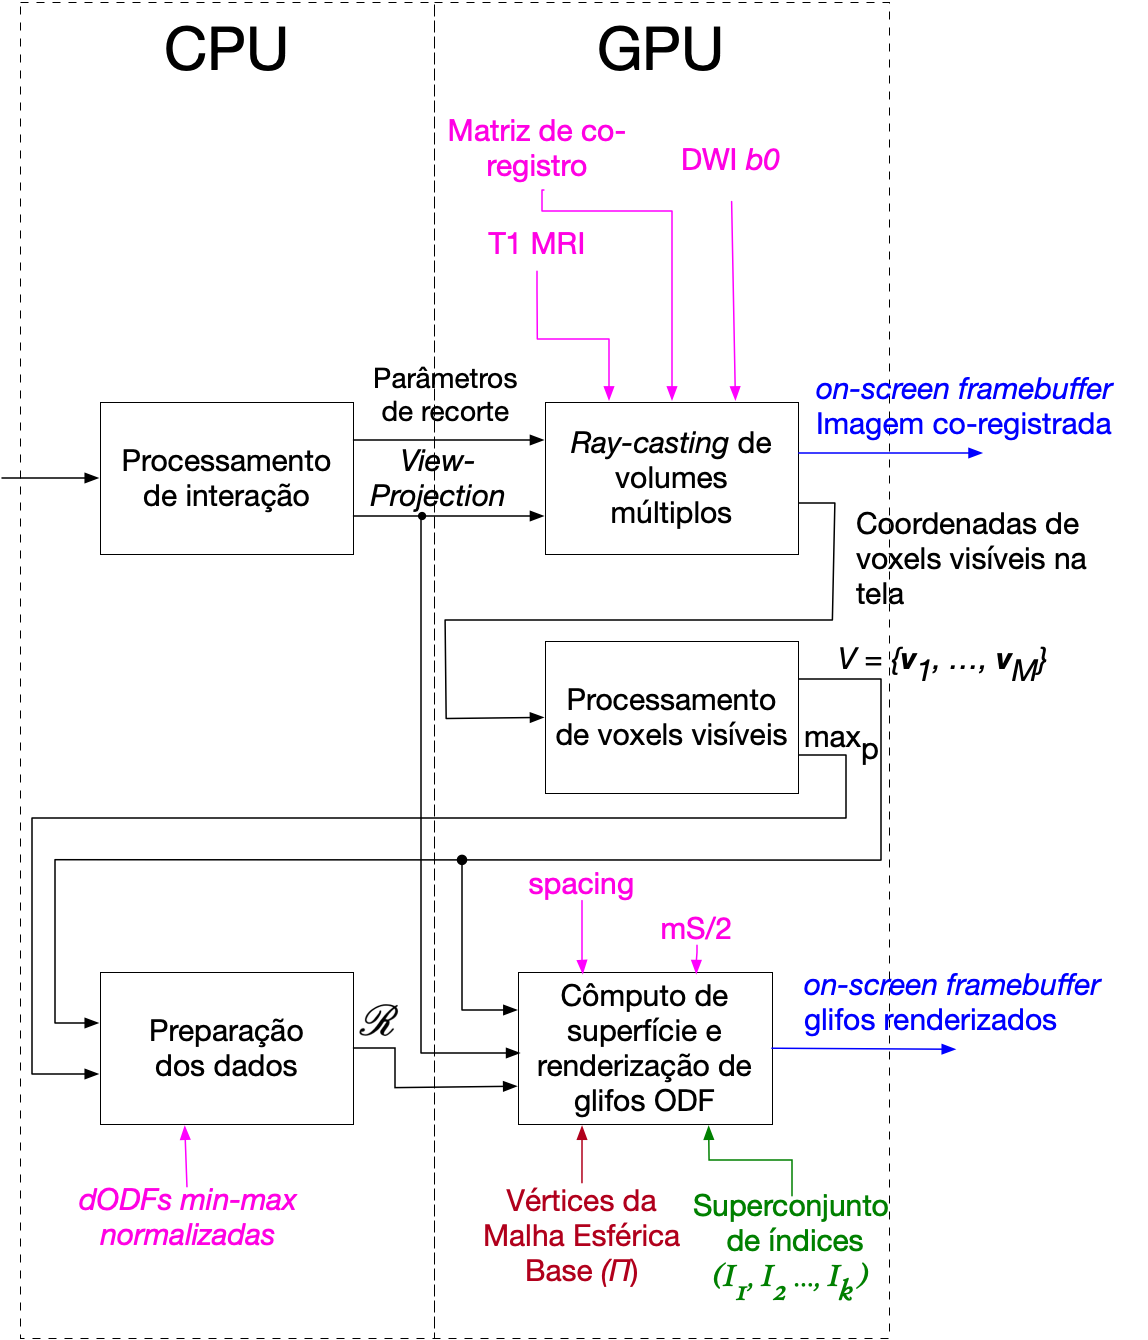
\includegraphics[width=.7\linewidth, angle=0]{figs/Esquema_Glifo/fluxograma_glifos_VMTK.png}
    \caption{
    Renderização multimodal para glifos ODF. A cor azul representa a saída a ser desenhada, armazenada no \textit{framebuffer} (FB); a cor magenta se refere a dados pré-computados. Os estágios de \textit{raycasting} do volume e processamento de \textit{voxels} visíveis estão descritos por \citeonline{voltoline2021}. O estágio de preparação dos dados de ODF e renderização de glifos ODF estão descritos na Seção \ref{sec::renderizacao_de_glifos_ODF}.
    }
    \label{fig::vmtk_simplified}
\end{figure}

Nossa solução para minimizar a transferência de dados consiste em explorar a resolução da percepção visual, o uso de renderização por instâncias, exploração da simetria de ODFs e o uso de memória de textura. Na Subseção \ref{ssec::geometria_base}, descrevemos a geometria base que é deformado por cada conjunto de amostras de ODF. Na Subseção \ref{ssec::atributos}, descrevemos o leiaute de atributos que otimiza o uso de memória da GPU e o seu acesso.

\subsection{Geometria base}
\label{ssec::geometria_base}

\subsubsection{Considerações iniciais}

As ODFs são amostradas a partir dos vetores normais dos pontos de uma malha base esférica $(\Pi, I)$, onde $\Pi = [P_1, P_2, \dots, P_N]$ consiste num conjunto de pontos não repetidos e o conjunto $I$ são os índices que referenciam os pontos de $\Pi$ para formar os triângulos que sintetizam a malha. Estabelecemos duas condições para a estrutura de dados, nas quais tiramos proveito da simetria de dados das ODFs e para que façamos a malha ser adaptativa para parâmetros de visualização. Estas condições tem impacto direto no tráfego de dados CPU-GPU, conforme discutido na Subseção \ref{ssec::atributos}.

A primeira condição, conforme já discutido no capítulo \ref{chapter::metodos_hardi} na forma de armazenamento de dados da ODF tira vantagem da simetria e armazena os pontos em metade de uma esfera. Propomos que os pontos simétricos em relação aos eixos coordenados de $\Pi$ estejam dispostos de forma consecutiva na memória, i. e. $P_{2i+2} = -P_{2i+1}$, $(0 \leq i \leq \frac{N-2}{2})$, o que nos leva a uma estrutura de dados $\Pi = [P_1, -P_1, P_3, -P_3, \dots, P_{N-3}, -P_{N-3}, P_{N-1}, -P_{N-1}]$.

A segunda condição objetiva fazer a geometria base do glifo ser adaptativa como uma sub-malha da malha esférica base. Seja $k$ o número de sub-malhas de $(\Pi, I)$, onde cada sub-malha é denotada por $(\Pi_i, I_i)$,  $(0 \leq i < k)$, adicionalmente, o número de pontos das sub-malhas é crescente de acordo com os sub-índices, i.e. se $(0 \leq i < j < k)$, implica $|\Pi_j| > |\Pi_i|$. Sugerimos que cada sub-malha $(\Pi_i, I_i)$ seja simétrica em relação a origem e os primeiros $|\Pi_i|$ elementos na estrutura de dados de $\Pi$ corresponda aos elementos de $\Pi_i$. Note que esta condição também implica que, para $i$, $j$ tais $0 \leq i < j < k$, $\Pi_i$ é subconjunto de $\Pi_j$.

\subsubsection{Formulação da geometria e estruturação de dados}
\label{sssec::formulação_da_geometria_e_estruturação_de_dados}

\todo[inline]{O procedimento de subdivisão não ficaria melhor no Cap. 2 quando se apresenta diferentes alternativas de subdivisões? Este procedimento entra como subdivisões uniformes}

Conforme mencionado no capítulo \ref{chapter::metodos_hardi}, escolhemos o conjunto de malhas derivada da $2^k$-ésima ordem de tesselação do icosaedro. O algoritmo para obtermos a tesselação de $2^k$-ésima ordem é um processo iterativo repetido $k$ vezes que se inicia com o icosaedro. Cada triângulo da malha é subdividido em quatro em cada iteração, onde os novos novos vértices adicionados são computados pela projeção da mediana dos pares de pontos conectados por uma aresta na esfera. Assim, o conjunto de vértices da $2^k$-ésima ordem contém todos os vértices das iterações anteriores. Adicionalmente, são todos simétricos com relação a origem. O processo de subdivisão de um triângulo está ilustrado na Fig. \ref{fig::triangle_icosahedron} e o algoritmo para se obter esta categoria de malha pode ser encontrado em \citeonline{luna2012}. Adicionalmente, a Fig. \ref{fig::icosphere} do Capítulo \ref{chapter::metodos_hardi} ilustra malhas esféricas desta categoria.

\begin{figure}[htb]
    \centering
    %\rule{6cm}{3cm}
    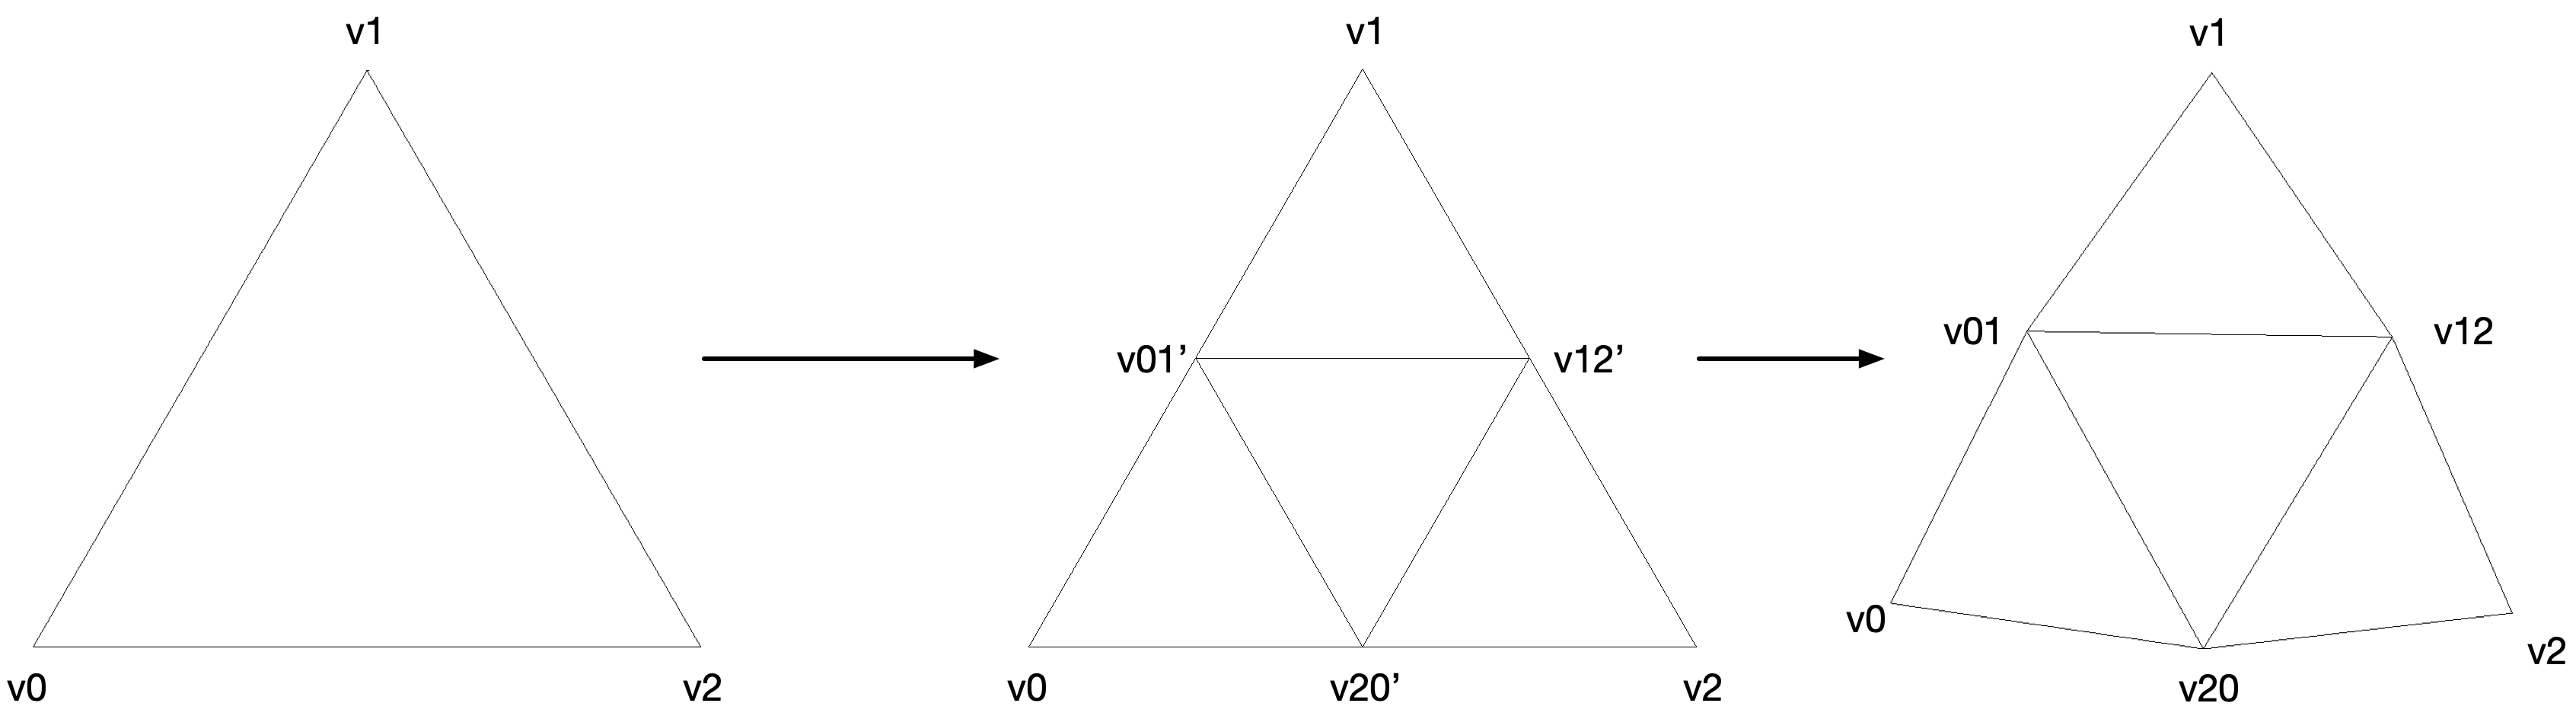
\includegraphics[width=1.0\linewidth, angle=0]{figs/Esquema_Glifo/ico_subdivision.png}
    \caption{
    Subdivisão de um triângulo para formar quatro na formação da malha esférica a partir da tesselação de $2^k$-ésima ordem a partir da partir da $2^{k-1}$-ésima. O triangulo formado pelos vértices $v0$, $v1$ e $v2$ é subdividido em quatro, onde as medianas  $v01'$, $v12'$ e $v20'$ são computadas e suas respectivas projeções na esfera $v01$, $v12$ e $v20$ são adicionados ao conjunto de vértices.
    }
    \label{fig::triangle_icosahedron}
\end{figure}

Há dois problemas adicionais que precisamos enfrentar no que diz respeito a obtenção de malhas esféricas através da subdivisão do icosaedro. O primeiro é garantir que os vértices simétricos estejam de forma consecutiva na memória e o segundo diz respeito a que não haja repetição de pontos em $\Pi$. O algoritmo para subdivisão do icosaedro em \citeonline{luna2012} insere vértices repetidos, pois há diversos pares de pontos conectados que definem mais de um triângulo.

A nossa abordagem para resolver esse problema consiste em identificar e deletar pontos replicados para termos somente uma amostra de cada em $\Pi$ e, após isso, ordenar o conjunto de dados $\Pi$ para que os simétricos estejam de forma consecutiva na memória, e essa mudança de estrutura de dados tem que ser compensada no conjunto de índices $I$. Para resolver estes problemas, propomos dois algoritmos que resolvem essas questões de forma genérica que são executados após cada iteração da subdivisão do icosaedro. O Algoritmo \ref{alg::tira_redundancia_pontos} certifica que os pontos redundantes são removidos, e o Algoritmo \ref{alg::reordena_simetricos} certifica que os pontos simétricos estarão em sequência na memória.

\begin{algorithm}
\caption{Algoritmo para retirada de pontos repetidos em estrutura de dados de vértices}
\label{alg::tira_redundancia_pontos}
\begin{algorithmic}[1]
\Procedure{ShrinkVertexSet}{$\Pi$, $I$}
 \State $I' \gets \{0, 1, 2, ..., |\Pi| - 1\}$
\State $i \gets 0$
\While{$i < |\Pi| - 1$} \label{alg::svs_pt1_inicio}
    \State $j \gets i + 1$
    \While{$j < |\Pi|$}
        \If {$\Pi[i] = \Pi[j]$}
            \State $I'[j] \gets i$
        \EndIf
        \State $j \gets j + 1$
    \EndWhile
    \State $i \gets i + 1$
\EndWhile \label{alg::svs_pt1_fim}
\State $\Pi_{size} \gets |\Pi|$
\State $i \gets 0$
\While{$i < \Pi_{size} - 1$} \label{alg::svs_pt2_inicio}
    \State $j \gets i + 1$
    \While{$j < \Pi_{size}$}
        \If{$\Pi[i] = \Pi[j]$}
            \State DELETE $\Pi[j]$ \label{alg::delete}
            \ForEach{$c \in I'$ \textbf{and} $c > j$}
                \State $c \gets c - 1$
            \EndFor
            \State $j \gets j - 1$
            \State $\Pi_{size} \gets \Pi_{size} - 1$
        \EndIf
        \State $j \gets j + 1$
    \EndWhile
    \State $i \gets i + 1$
\EndWhile \label{alg::svs_pt2_fim}
\ForEach{$c \in I$} \label{alg::resetI}
    \State $c \gets I'[c]$
\EndFor
\EndProcedure
\end{algorithmic}
\end{algorithm}

 \begin{algorithm}
 \caption{Pseudocódigo que sequencia vértices simétricos na memória}
 \label{alg::reordena_simetricos}
 \begin{algorithmic}[1]
 \Procedure{AlignSymmetricalMesh}{$\Pi$, $I$}
 \State $I' \gets \{0, 1, 2, ..., |\Pi| - 1\}$
 \State $i \gets 0$
 \While{$i < |\Pi| - 1$} 
     \State $j \gets i + 1$
     \While{$j < |\Pi|$}
         \If {$\Pi[i] = -\Pi[j]$}
             \State Swap($\Pi[i+1]$, $\Pi[j]$) \label{alg::troca}
             \ForEach{$c \in I$} \label{alg::compensacao_inicio}
                \If{$c = i+1$}
                    \State $c \gets j$
                    \State CONTINUE
                \ElsIf{$c = j$}
                    \State $c \gets i+1$
                    \State CONTINUE
                \EndIf
             \EndFor
             \State \textbf{break}
         \EndIf 
         \State $j \gets j + 1$
         \If {$j = |\Pi|$}
            \State \textbf{return} ERROR\_MESH\_NOT\_SYMMETRICAL
         \EndIf
     \EndWhile \label{alg::compensacao_fim}
     \State $i \gets i + 2$
\EndWhile
 \EndProcedure
 \end{algorithmic}
 \end{algorithm}
 
 O Algoritmo \ref{alg::tira_redundancia_pontos} pode ser dividido em duas partes e tem no vetor $I'$ o seu ponto crucial de funcionamento. Cada $I'[i]$ armazena está associado ao $i$-ésimo elemento de $\Pi$. Após a deleção dos elementos repetidos em $\Pi$, $I[i]$ guarda o índice do ponto que é igual a $\Pi[i]$ antes da deleção dos vértices repetidos.
 
 A primeira parte do algoritmo (Linhas \ref{alg::svs_pt1_inicio} até \ref{alg::svs_pt1_fim}) consiste trocar os vértices repetidos apontados por $I'$ para a sua primeira ocorrência em $\Pi$, visto que as demais ocorrências irão ser apagadas. A segunda parte do algoritmo (Linhas \ref{alg::svs_pt2_inicio} até \ref{alg::svs_pt2_fim}) consiste na deleção dos vértices repetidos, o comando DELETE na linha \ref{alg::delete} considera que a o processo de deleção do elemento consiste em deslocar os seus elementos conseguintes na memória para o endereço anterior\footnote{O funcionamento descrito é similar à função std::erase aplicada a classe std::vector em C++}, consequentemente, isto é compensado no conjunto de índices $I'$ pelo decremento de todos os índices apontados com valores maiores do que $j$. Na linha \ref{alg::resetI}, o elementos no conjunto de índices $I$ são corrigidos para referenciar para nova versão sem redundância de $\Pi$.
 
O Algoritmo \ref{alg::reordena_simetricos}, consiste na detecção dos simétricos e a troca de posição de pontos em índices ímpares para os simétricos dos índices pares em $\Pi$ (Linha \ref{alg::troca}) na posição anterior e a compensação no conjunto de índices $I$ (Linhas \ref{alg::compensacao_inicio} até \ref{alg::compensacao_fim}).

Sendo assim, o Algoritmo \ref{alg::setIcosahedroBase} mostra os procedimentos para subdivisão do icosaedro, bem como onde os algoritmos \ref{alg::tira_redundancia_pontos} e \ref{alg::reordena_simetricos} se situam. A variável $k$ representa a quantidade de iterações, $\mathbf{I}$ é o superconjunto que contém os conjuntos de índices para diferentes resoluções do glifo e $\Pi$ a lista de vértices do icosaedro tesselado de ordem $2^k$.

Nas linhas \ref{alg::subdivide_icosahedron} e \ref{alg::project_onto_sphere}, temos o algoritmo de subdivisão dos triângulos em quatro e sua projeção na esfera \cite{luna2012}, obtidos como ilustrado na Fig. \ref{fig::triangle_icosahedron}, adicionalmente, os novos vértices gerados são alocados após o fim da estrutura de dados dos vértices base, o que faz com que, os vértices do icosaedro estejam situados no início da estrutura, seguidos dos vértices gerados pela primeira subdivisão, depois dos vértices gerados na segunda subdivisão e assim sucessivamente.

 \begin{algorithm}
 \caption{Pseudocódigo que gera diferentes esferas a partir de tesselações de ordem $2^k$ do icosaedro.}
 \label{alg::setIcosahedroBase}
 \begin{algorithmic}[1]
 \Function{SetIcosahedronSet}{$k$}
 \State $\mathbf{I} = \{I_0, I_1, ..., I_{k-1}, I\}$
 \State $(\Pi, I) = \text{(Icosahedron.Vertices, Icosahedron.Indices)}$  \cite{luna2012} \label{alg::init_icosahedron}
 \State $i \gets 0$
 \While{$i < k$}
    \State ShrinkVertexSet($\Pi, I$)
    \State AlignSymmetricalMesh($\Pi, I$)
    \State $I_i \gets I$
    \State ($\Pi$, $I$) = Subdivide($\Pi, I$) \cite{luna2012}  \label{alg::subdivide_icosahedron}
    \State ($\Pi$) = ProjectOntoSphere($\Pi$) \cite{luna2012} \label{alg::project_onto_sphere}
    \State $i \gets i + 1$
\EndWhile
    \State \textbf{return} $(\Pi, \mathbf{I})$
 \EndFunction
 \end{algorithmic}
 \end{algorithm}
 

Assim, definindo $(\Pi, I)$ para ser a $2^{k}$-ésima ordem de tesselação para ser a malha esférica base e mantendo cada conjunto de índices de menor ordem a cada iteração, temos um conjunto de $k$ sub-malhas $(\Pi_0, I_0), (\Pi_1, I_1), ..., (\Pi_{k-1}, I_{k-1})$ definidos como as tesselações de $1^{a}$, $2^{a}$, ... $2^{k-1}$-ésima ordem. As Eq. \ref{eq::2ordem_icosphere_vertices}\footnote{Note que esta equação é a Eq. \ref{eq::icosa_samples} adaptada para $2^k$-ésima ordem de tesselação do icosaedro} e \ref{eq::2ordem_icosphere_triangulos} computam a quantidade de vértices e triângulos para esta categoria de malha em função da tesselação de ordem $2^k$, respectivamente.

\begin{equation}
\label{eq::2ordem_icosphere_vertices}
V = 10\times 4^k + 2
\end{equation}

\begin{equation}
\label{eq::2ordem_icosphere_triangulos}
\tau = 20\times 4^k
\end{equation}

Assim como mencionado no capítulo \ref{chapter::metodos_hardi}, por questões de memória, recomendamos k = 3, ou no máximo 4. Assim, formulamos a estrutura de dados que satisfaz as duas condições que estabelecemos a princípio, e é tal que os primeiros 12 elementos correspondem aos vértices do icosaedro, os 42 primeiros elementos correspondem aos vértices da $2^a$ ordem de tesselação, os 162 primeiros elementos correspondem a $4^a$ ordem de tesselação, os primeiros 642 elementos correspondam a $8^{a}$ ordem de tesselação, e, adicionalmente, os pontos simétricos são agrupados em sequencia na memória.

A estrutura de dados $\Pi$, e $I$, além dos índices que triangulam todas as sub-malhas, contidos ao superconjunto $\mathbf{I}$ no Algoritmo \ref{alg::setIcosahedroBase}, são enviados à GPU uma vez. Uma vez que os dados estão na GPU, e visando eficiência no processamento, sem comprometer a qualidade visual, escolhemos adaptativamente a geometria base entre estas malhas por um procedimento heurístico computado em tempo de execução baseado em $max_p$.

\subsection{Escolha automática da geometria base}
\label{sssec::escolha_automatica_da_geometria_base}

A escolha da geometria base é baseada no \textit{trade-off} de \citeonline{voltoline2021}, que indica a quantidade mínima de triângulos para dado um $max_p$, que é dado por $\tau \geq 8\sqrt{max_p}$  ($max_p > 0$). Este \textit{trade-off} estabelece a quantidade mínima de triângulos a ser utilizada na malha que não sacrifica a qualidade de imagem dos glifos. Derivamos uma expressão para a escolha da sub-malha da malha esférica base a partir do caso de igualdade do \textit{trade-off}, no qual substituímos a quantidade de triângulos como uma função da ordem de tesselação do icosaedro e mapeamos o icosaedro para o caso $max_p = 0$. A expressão base está na Eq. \ref{eq::icosa_order_base}:

\begin{equation}
\label{eq::icosa_order_base}
     20\times 4^k - 20\times 4^0 = 8\sqrt{max_p}
\end{equation}

Derivamos $t$ ($t \leq k$) na Eq. \ref{eq::icosa_order} como a ordem de tesselação do icosaedro escolhida. Como $t$ é inteiro positivo, para satisfazer o \textit{trade-off} de \citeonline{voltoline2021}, arrendondamos o valor para cima.

\begin{equation}
\label{eq::icosa_order}
     t = \lceil \frac{1}{2}\log_2{(\frac{2}{5}\sqrt{max_p} + 1)} \rceil
\end{equation}

Para geometria base derivada da $2^t$-ésima ordem de tesselação, devemos ser atentos a dois procedimentos na seleção da malha em tempo de execução. O primeiro consiste na ativação do seu respectivo conjunto de índices para triangulação. O segundo consiste em setar a quantidade de dados de ODF por glifo enviado à GPU como uma função de sua quantidade de vértices, o que será discutido mais a frente, na Subseção \ref{ssec::atributos}.

\subsubsection{Fator de escala para geometria}

Finalmente, sugerimos escalar a a malha base pelo fator de escala $mS$ para proporcionar a máxima ocupância em tela, fazendo o glifo, cuja ODF está contida no intervalo $[0, 1]$, caber no seu respectivo \textit{voxel}:

\begin{equation}
\label{eq:spacings}
mS = min(spacing_x, spacing_y, spacing_z)
\end{equation}


onde $spacing_x$, $spacing_y$, $spacing_z$ é o espaço entre duas amostras adjacentes nos eixos x, y e z, respectivamente.





%The vertices and amount of triangles and the expression for the vertices and triangles number for each $2^k$ tessellation are in Table \ref{tab::icosahedron_set}. In practice, we recommend $k$ to be equal to 3 or 4, at most. Values of above those may incur a prohibitive amount of memory for pre-computed ODF samples in a DWI.

\subsection{Atributos}
\label{ssec::atributos}



Para renderizarmos $M$ glifos com um comando de desenho, usamos instanciação de GPU. A geometria base selecionada, referente a $2^t$-ésima ordem de tesselagem do icosaedro é instanciada por um vetor de translação e amostras de ODF.

\subsubsection{Posicionamento}

Para $M$ \textit{voxels} visíveis, enviamos os vetores de translação como um atributo por instância, que é computado em função das coordenadas de \textit{voxel} $V(v_x, v_y, v_z)$ como:

\begin{align}
 \label{eq::translation}
    dx = (v_x + 0.5).spacing_x \nonumber\\
    dy = (v_y + 0.5).spacing_y \\
    dz = (v_z + 0.5).spacing_z \nonumber
\end{align}

Note que os dados de voxel visíveis retornados pelo algoritmo é armazenado em um buffer na GPU. Este dado é utilizado diretamente no algoritmo de renderização no \textit{vertex shader} para cômputo do atributo de translação.

\subsubsection{Dados de ODF}
\label{sssec::dados_de_odf}

Como mencionado no capítulo \ref{chapter::metodos_hardi}, aproveitamos a simetria dos dados de ODF para organizarmos os dados no domínio de um hemisfério. Para o voxel de coordenadas índice $\mathbf{r}$, os elementos são organizados como $\boldsymbol{\psi}(\mathbf{r}) = [
\psi(\mathbf{r}, \mathbf{n}_1),
\psi(\mathbf{r}, \mathbf{n}_3), ...,
\psi(\mathbf{r}, \mathbf{n}_{N-3}),
\psi(\mathbf{r}, \mathbf{n}_{N-1})]^T$. Onde cada elemento na K-ésima posição $\psi(\mathbf{r}, \mathbf{n}_{2K-1})$ desloca os pontos $P_{2K-1}$ e seu simétrico $P_{2K}$ na geometria base instanciada. Note que no capítulo \ref{chapter::metodos_hardi}, o armazenamento de amostras em um metade de uma esfera tem o objetivo de economia de memória, enquanto neste capítulo, tem o objetivo de minimizar o tráfego de dados CPU-GPU.

Para a geometria base escolhida, geramos uma matriz com os dados de ODF enviados à GPU como a matriz $\mathbf{R}_{\frac{V}{2}xM}$ (Eq. \ref{eq::R}), onde $V$ é o numero de vértices da geometria base, dado por $10 \times 4^t + 2$ (Eq. \ref{eq::2ordem_icosphere_vertices}). A $j$-ésima coluna consiste nos primeiros $V/2$ elementos de $\boldsymbol{\psi}(\mathbf{d_j})$. $\mathbf{R}$ é enviado à GPU como uma textura 2D de formato RGBA.

\begin{equation}
\label{eq::R}
\mathbf{R} = 
\begingroup % keep the change local
\setlength\arraycolsep{2pt}
\begin{bmatrix} 
    \psi(\mathbf{d}_{1}, \mathbf{n}_1) &
    \psi(\mathbf{d}_{2}, \mathbf{n}_1) & \cdots & 
    \psi(\mathbf{d}_{M}, \mathbf{n}_1)  \\
    
    \psi(\mathbf{d}_{1}, \mathbf{n}_3) &
    \psi(\mathbf{d}_{2}, \mathbf{n}_3) & \cdots & 
    \psi(\mathbf{d}_{M}, \mathbf{n}_{3}) \\ \vdots & \vdots & \vdots & \vdots  \\
    
    \psi(\mathbf{d}_{1}, \mathbf{n}_{V-1}) & 
    \psi(\mathbf{d}_{2}, \mathbf{n}_{V-1}) & \cdots & 
    \psi(\mathbf{d}_{M}, \mathbf{n}_{V-1})
\end{bmatrix}.
\endgroup
\end{equation}

Cada \textit{texel} no formato RGBA suporta quatro valores. Agrupamos os valores escalares da j-ésima coluna $[
\psi(\mathbf{d}_{j}, \mathbf{n}_1),
\psi(\mathbf{d}_{j}, \mathbf{n}_3), ...,
\psi(\mathbf{d}_{j}, \mathbf{n}_{V-3}),
\psi(\mathbf{d}_{j}, \mathbf{n}_{V-1})
]^T$ de quatro em quatro, como mostrado na Fig. \ref{fig::texelfetch}. Consequentemente, em cada acesso de \textit{texel}, temos quatro valores escalares $
\psi(\mathbf{d}_{j}, \mathbf{\mathbf{n}_{8K+1}})$ (R), $
\psi(\mathbf{d}_{j}, \mathbf{\mathbf{n}_{8K+3}})$ (G), $
\psi(\mathbf{d}_{j}, \mathbf{\mathbf{n}_{8K+5}})$ (B), $
\psi(\mathbf{d}_{j}, \mathbf{\mathbf{n}_{8K+7}})$ (A). Nos quais deslocamos quatro pares de pontos simétricos na geometria base $P_{8K+1}$, $-P_{8K+1}$, $P_{8K+3}$, $-P_{8K+3}$, $P_{8K+5}$, $-P_{8K+5}$, $P_{8K+7}$, $-P_{8K+7}$ para o j-ésimo glifo visível (também j-ésima instância). Desta forma, as dimensões da textura com dados ODF é $ \frac{V/2}{4} \times M$. Se $\frac{V}{2}$ não é divisível por quatro, é necessário inserir mais linhas abaixo da última com valores \textit{dummy}, para que o número de linhas se torne divisível, o que certifica que cada coluna de $\mathbf{R}$ possa ser acessada com o índice de instância na GPU.

\begin{figure}[ht]
%\subfigcapskip = -5pt
    \centering
    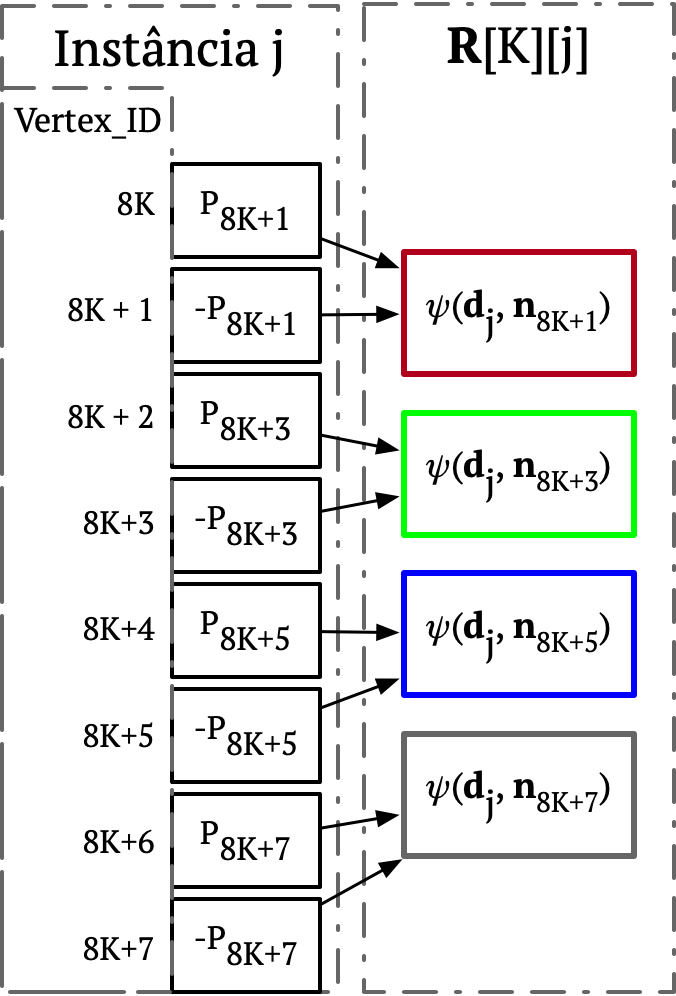
\includegraphics[width=.45\linewidth, angle=0]{figs/Esquema_Glifo/texellookup.png}
    \caption{Ilustração do acesso nas componentes RGBA em \textit{texel} na textura \textbf{R} no índice $K$ e $j$. O \textit{texel} é acessado pelas threads que processam os vertices de índices 8K, 8K+1, ..., 8K+7 em uma instância $j$. Os blocos de contorno vermelho, azul, verde e cinza ilustram as componentes R,G,B e A do \textit{texel}, respectivamente.}
    \label{fig::texelfetch}
   %\hspace{1pt}
\end{figure}

Os dados de ODF são acessados no \textit{vertex shader}, quando cada glifo da $j$-ésima instância é processada. Os \textit{texels} com índice de coluna $K = \lfloor\frac{Vertex\_ID}{8} \rfloor$ são acessados para deslocar oito pontos. Usamos a função \textit{texelFetch} para acessar diretamente a textura de ODF utilizando coordenadas não-normalizadas $(j, \lfloor\frac{Vertex\_ID}{8} \rfloor)$. O valor utilizado para \textit{lookup} da componente  para deslocar o seu respectivo ponto na geometria base no \textit{vertex shader} é acessível pela análise do resto da divisão por oito do Vertex\_ID, como ilustrado na Fig. \ref{fig::texelfetch}. Adicionalmente, utilizando a notação via colchetes, onde as componentes R, G, B e A são mapeados nos índices 0, 1, 2 e 3, respectivamente, o escalar de ODF pode ser mapeado por $\lfloor (Vertex\_ID \mod{8})/2 \rfloor$\footnote{A função em OpenGL para \textit{lookup} em função dos índices de instância e vértice é dada por texelFetch($\mathbf{R}$,ivec2((gl\_VertexID)/8, gl\_InstanceID), 0)[(gl\_VertexID\%8)/2]}.

\subsection{Síntese}

Podemos sintetizar as transformações aplicadas a cada vértice $P_K$ em coordenadas homogêneas na $j$-ésima instância por uma multiplicação matricial no \textit{vertex shader} por uma matriz $G_{Kj}$. Esta matriz pode ser sintetizada da seguinte forma:

\begin{equation}
    G_{Kj} = \mathbf{M_{vp}}\cdot M_D \cdot M_S \cdot M_{Kj}
\end{equation}

onde $M_{kj}$ é a matriz que escalona o ponto $P_K$ na $j$-ésima instância por $\psi(\mathbf{d}_j, \mathbf{n}_k)$, $M_S$ se refere a transformação de escala, dado por Eq. \ref{eq:spacings}, $M_D$ é a matriz de translação do glifo, centrado na origem para o centro do seu respectivo \textit{voxel} no espaço do volume, dado pela Eq. \ref{eq::translation}, e, adicionalmente, $\mathbf{M_{vp}}$ é a matriz \textit{view-projection}, que configura parâmetros de visão e projeção.

\section{Experimentos, resultados e discussão}
\label{sec::experimentos}

Propomos um experimento para avaliar aspectos visuais do nosso algoritmo de esquema de renderização em comparação à superquádricas e medições de performance para atestarmos a interatividade do algoritmo de renderização. As medições foram feitas em um computador Macbook Pro Retina 13', com processador Intel Core i5 Dual-Core 2.7GHz, processador gráfico integrado Intel Iris Graphics 6100 1536 MB e memória RAM de 8 GB 1867 MHz DDR3.

As imagens geradas no experimento foram coletadas a partir o WU-Minn HCP Retest Data pelo \textit{Connectome Project Consortium} \cite{essen2012}.

Os dados de difusão foram adquiridos em um \textit{scanner} Siemens 3T Skyra. A aquisição é \textit{multi-shell} com 90 gradientes de ponderação de difusão para cada \textit{shell} $b = 1000, 2000$ e $3000 s/mm^2$, e estas direções são uniformemente distribuídas nos três \textit{shells}, e adicionalmente foram escaneados 6 aquisições $b0$ para cada \textit{shell}, totalizando 288 imagens. Os dados foram pré-processados com a \textit{pipeline} de pré-processamento para dados de difsão do Human Connectomme Project (HCP) \cite{glasser2013}. A aquisição pré-processada é representada por um volume $145\times 174\times  145$ com espaço entre amostras de $1.25\times 1.25 \times 1.25$mm.

A aquisição anatômica ponderada em T1 foi também pré-processada utilizando a pipeline de pré-processamento do HCP \cite{glasser2013}. Como o seu respectivo DWI, é representada por um volume $145\times 174\times  145$ com espaço entre amostras de $1.25\times 1.25\times 1.25$mm.

As ODFs foram obtidas através do GQI \cite{yeh2010} e min-max normalizadas o fator $\sigma \sqrt{6D}$ que utilizamos é de 0,0239. As amostras foram computadas com base no hemisfério da $8^{a}$ ordem de tesselação do icosaedro e armazenadas na CPU, como mostrado no Capítulo \ref{chapter::metodos_hardi}, gerando um total de 321 amostras por \textit{voxel}.

\subsection{Aspectos Visuais}
\label{ssec::aspectos_visuais}

\subsubsection{Transição de Resolução}

Com o objetivo de evidenciar a diferença na resolução e quantidade de triângulos nas transições de geometria base, fizemos um experimento em que interagimos com o ambiente de visualização multimodal em que modificamos ajustamos o fator de escala na visualização tal que o $max_p$ mensurado esteja no limite da troca da a geometria base utilizada no glifo. Fig.  \ref{fig::multimodal_teste_zoom} ilustra experimento.

Fig. \ref{fig::multimodal_162_hollow} e \ref{fig::multimodal_642_hollow} correspondem aos mesmos glifos em Fig. \ref{fig::multimodal_162_filled} e \ref{fig::multimodal_642_filled}, respectivamente e estão apresentados para evidenciar a mudança na quantidade de triângulos em cada um deles. As imagens foram gerada a partir de uma janela $500 \times 500$ com uma diferença sutil no fator de escala entre ambas. Nas Fig. \ref{fig::multimodal_162_hollow} e \ref{fig::multimodal_162_filled}, o valor de $max_p$ é de 1394 \textit{pixels}, e em \ref{fig::multimodal_642_hollow} e \ref{fig::multimodal_642_filled}, é de 1409. De acordo com Eq. \ref{eq::icosa_order}, o limiar de mudança entre as geometrias é $max_p = 1406.25$.  O glifo mostra uma visão axial do corpo caloso, cujo comportamento de difusão ocorre predominantemente na direção esquerda-direita. Fig. \ref{fig::multimodal_teste_loc} mostra a localização da região mostrada em Fig. \ref{fig::multimodal_teste_zoom}.


\begin{figure}[ht]
    \centering
    %\rule{6cm}{3cm}
    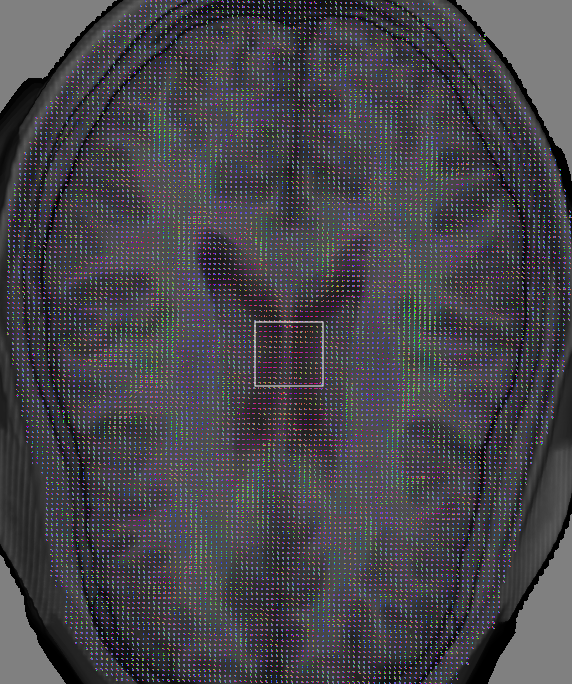
\includegraphics[width=.56\linewidth, angle=0]{figs/Esquema_Glifo/Teste_transicao/base_teste_zoom.png}
    \caption{MRI T1 anatômico co-registrado com DWI. A região dentro do contorno quadrado branco corresponde a região analisada na Fig. \ref{fig::multimodal_teste_zoom}.}
    \label{fig::multimodal_teste_loc}
\end{figure}


\begin{figure}[ht]
\centering
\captionsetup[subfloat]{farskip=0pt,nearskip=0pt}
    \subfloat[$4^a$ ordem de tesselação - apenas contornos dos triângulos]{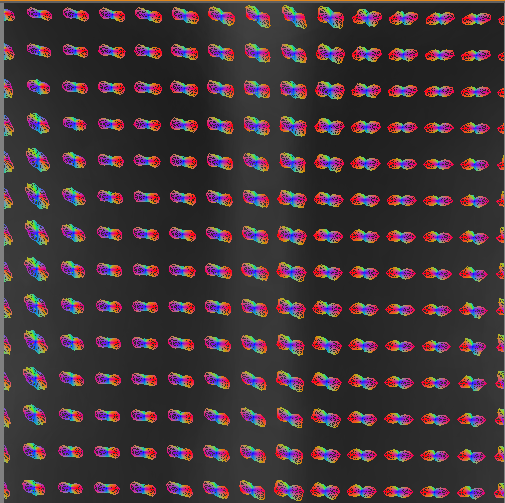
\includegraphics[width=.49\linewidth, angle=0]{figs/Esquema_Glifo/Teste_transicao/162_Hollow.png}
    \label{fig::multimodal_162_hollow}
    }
    \subfloat[$4^a$ ordem de tesselação - triângulos preenchidos] {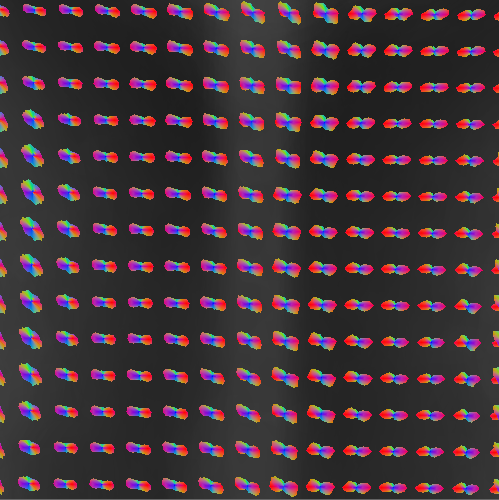
\includegraphics[width=.485\linewidth, angle=0]{figs/Esquema_Glifo/Teste_transicao/162_filled.png}
    \label{fig::multimodal_162_filled}
    }
    \hspace{1pt}
    \subfloat[$8^a$ ordem de tesselação - apenas contornos dos triângulos]{\includegraphics[width=.495\linewidth, angle=0]{figs/Esquema_Glifo/Teste_transicao/642_Hollow.png}
    \label{fig::multimodal_642_hollow}
    }
    \subfloat[$8^a$ ordem de tesselação - triângulos preenchidos] {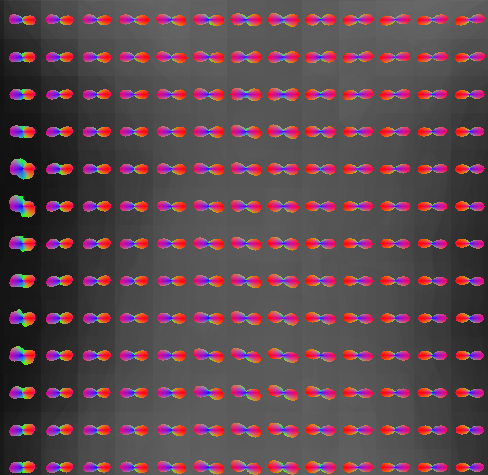
\includegraphics[width=.487\linewidth, angle=0]{figs/Esquema_Glifo/Teste_transicao/642_filled.png}
    \label{fig::multimodal_642_filled}
    }
    \caption{Ilustração da troca de resolução efetuada automaticamente a partir de $max_p$. A troca de resolução ocorre entre as geometrias base derivadas da $4^a$ (\ref{fig::multimodal_162_hollow} e \ref{fig::multimodal_162_filled}) e $8^a$ (\ref{fig::multimodal_642_hollow} e \ref{fig::multimodal_642_filled}) ordem de tesselação. A região ilustrada é do corpo caloso, que está em destaque na Fig. \ref{fig::multimodal_teste_loc}.
    }
    \label{fig::multimodal_teste_zoom}
\end{figure}

Podemos observar a suavidade em que a mudança de resolução ocorre. Observamos que os glifos com os triângulos preenchidos neste nível de resolução não apresentam efeitos característicos de malhas de baixa resolução e que a transição na resolução ocorre de forma sutil.

Adicionalmente, caso o usuário queira analisar os glifos mais de perto ou aumente o tamanho da janela, fazendo-a cobrir mais \textit{pixels}, o glifo é gerado a partir de uma malha suave o suficiente no qual ele tenha total liberdade para visualizar o comportamento das ODFs. Caso o usuário queira ter uma visão mais geral do volume com os glifos e diminua o fator de escala, diminuímos a resolução de cada glifo renderizado para aliviar o processamento computacional associado a cada um deles.


\subsubsection{Cruzamentos de Fibras}

Fig. \ref{fig::multimodal} ilustra uma fatia coronal na região do \textit{centrum semiovale} com um triplo cruzamento de fibras correspondentes do corpo caloso, \textit{corona radiata} e o fascículo longitudinal superior. A região apresenta cruzamentos de fibra conhecidos e é utilizada para análises qualitativas. Fig. \ref{fig::multimodal_highres} mostra que pode-se inferir sobre cada cruzamento de fibra nas regiões mais alongadas da superfície do glifo. Observe também que a resolução do glifo é diferente na Fig. \ref{fig::multimodal_lowres} em comparação a \ref{fig::multimodal_highres} e sua seleção é feita de forma automática. No fundo, há a renderização da ressonância anatômica ponderada em T1 co-registrada.

\begin{figure}[ht]
\centering
\captionsetup[subfloat]{farskip=0pt,nearskip=0pt}
    \subfloat[Fatia coronal de um MRI T1 co-registrado com DWI. A geometria base corresponde a $2^a$ ordem de tesselação do icosaedro.]{\makebox[1.2\width]{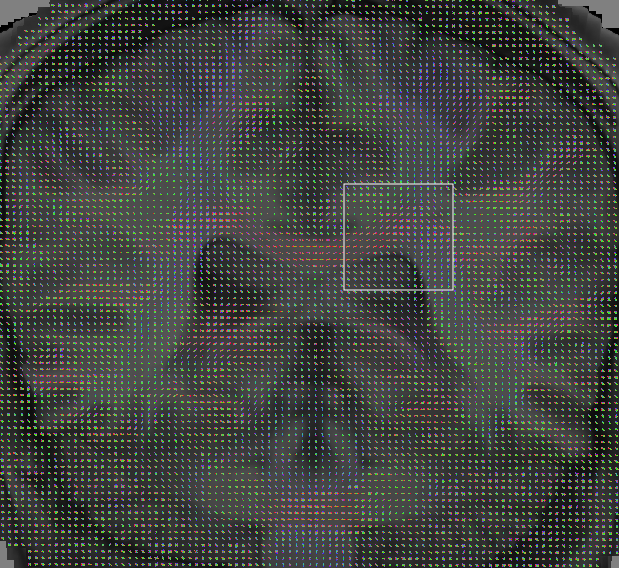
\includegraphics[width=.60\linewidth, angle=0]{figs/Esquema_Glifo/LowResImgHighlighted.png}}
    \label{fig::multimodal_lowres}
    }
    \hspace{1pt}
    
    \subfloat[Cruzamento entre fibras de corpo caloso (direita-esquerda), \textit{corona radiata} (descendente-ascendente) e fascículo longitudinal superior (anteroposterior - normal ao plano da página). A geometria base é a $8^a$ ordem de tesselação do icosaedro.] {\makebox[2.0\width]{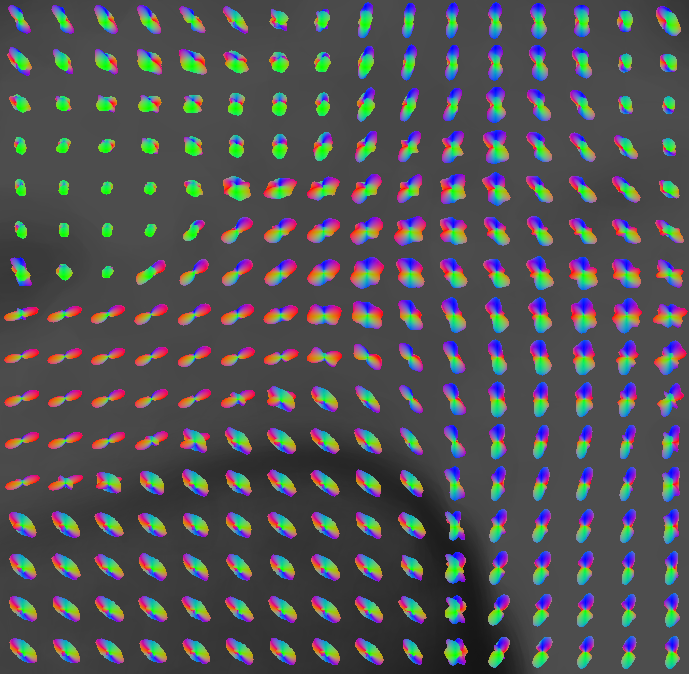
\includegraphics[width=.45\linewidth, angle=0]{figs/Esquema_Glifo/HighResImg.png}
    \label{fig::multimodal_highres}}
    }
    \caption{ Glifos ODF integrados ao ambiente de visualização multimodal para MRI. A imagem se refere a um MRI T1 cor-registrado a o seu respectivo DWI. \ref{fig::multimodal_highres} corresponde a região dentro do contorno de cor branca em \ref{fig::multimodal_lowres}.}
    \label{fig::multimodal}
\end{figure}



\citeonline{voltoline2021} evidenciaram que a sua respectiva renderização multimodal para superquádricas do DTI pode ajudar no processo de escolhas referentes a sementes em tractografia, em comparação à mapas de anisotropia codificados por cor. Fig. \ref{fig::multimodal_superquadric} ilustra a mesma região de Fig. \ref{fig::multimodal_highres} com superquádricas. Note que os glifos apresentam o mesmo problema presente no próprio DTI: em cruzamentos de fibra, a distribuição de fibras subjacente não é inferível. Pode-se perceber isto na região de cruzamento de fibras enquanto nos glifos ODF, é possível inferir sobre a natureza do cruzamento de fibras, nas superquádricas, o glifo apresenta uma forma retangular suave e não gera a possibilidade de inferir sobre as fibras que compõem o cruzamento.


\begin{figure}[ht]
    \centering
    %\rule{6cm}{3cm}
    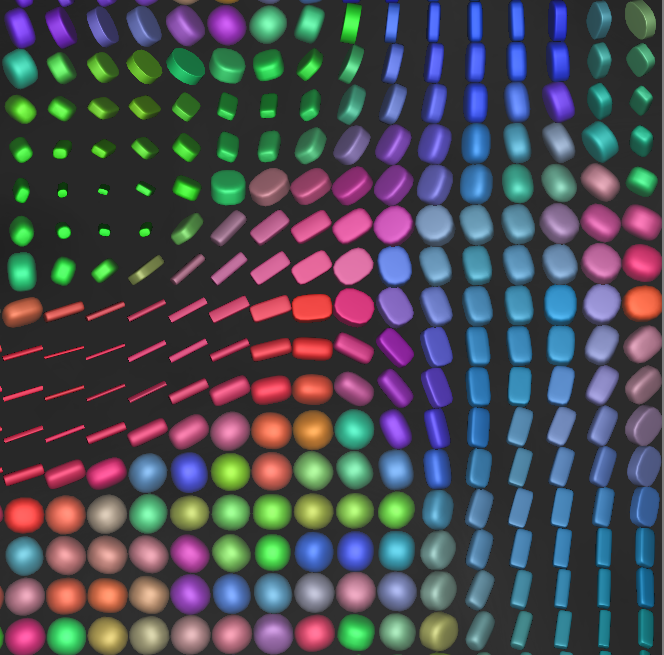
\includegraphics[width=.35\linewidth, angle=0]{figs/Esquema_Glifo/HighResImgSuperquadric.png}
    \caption{ Renderização multimodal para superquádricos do DTI. A imagem corresponde à mesma região em Fig. \ref{fig::multimodal_highres}.}
    \label{fig::multimodal_superquadric}
\end{figure}

\subsection{Performance}
\label{ssec::performance}

Mensuramos o tempo de performance da renderização multimodal de glifos para ODF. O número de glifos é modificado pela mudança do fator de \textit{zoom}. Evidentemente que, maior o fator de \textit{zoom}, menor a quantidade de glifos, maior é a ocupância dos \textit{voxels} na tela, o que aumenta a resolução do glifos. A resolução da janela de saída é de $850\times 850$ e o número de glifos visíveis varia de 12 e 13360. A resolução dos glifos varia com a utilização de geometria base da $2^a$ ordem de tesselação do icosaedro (menor nível de detalhe, Fig. \ref{fig::multimodal_lowres}) até a $8^a$ (maior nível de detalhe, Fig. \ref{fig::multimodal_highres}). O FPS do esquema de renderização em função da quantidade de glifos renderizados e parâmetros relacionados de fator de escala e geometria base utilizados estão listados na Tabela \ref{tab::glyph_info_experiment}, onde atestamos que o esquema renderiza em taxas interativas \cite{nielsen1994}.



\begin{table}[]
\centering
\begin{tabular}{|cccc|}
\hline
\textbf{FPS} & \textbf{Fator de escala} & \textbf{\# glifos} & \textbf{\begin{tabular}[c]{@{}c@{}}Ordem de \\ tesselação\end{tabular}} \\ \hline
33.85 & 92.27 & 12     & 8 \\
33.69 & 61.51 & 20     & 8 \\
34.75 & 41.01 & 42     & 8 \\
34.66 & 27.34 & 90     & 8 \\
36.29 & 18.23 & 182    & 8 \\
35.97 & 12.15 & 380    & 8 \\
32.98 & 8.10  & 870    & 4 \\
35.83 & 5.40  & 1892   & 4 \\
31.92 & 3.60  & 4160   & 4 \\
22.94 & 2.40  & 9032   & 4 \\
17.15 & 1.52  & 13205  & 2  \\
\hline
\end{tabular}
\caption{Esquema de renderização multimodal com glifos de ODF renderizados em uma imagem $850\times 850$. O número de vértices e triângulos utilizados são computados de acordo com as Eq. \ref{eq::2ordem_icosphere_vertices} e \ref{eq::2ordem_icosphere_triangulos}. A Fig. \ref{fig::multimodal_lowres} do apêndice se refere a imagem gerada pelos parâmetros da última linha da tabela}
\label{tab::glyph_info_experiment}
\end{table}

\subsection{Renderização por Fatias}
\label{ssec::renderizacao_por_fatias}

Podemos comparar nossa abordagem com a de \citeonline{shattuck2008}, uma vez que ambas são baseadas em polígonos, onde amostras de ODF deformam uma malha esférica. Em sua abordagem, \citeonline{shattuck2008} armazena ODFs como coeficientes de funções base na CPU e os glifos são computados e visualizados em fatias, que são visualizadas de forma ortogonal. O cômputo da forma dos glifos é feito na CPU, onde o valor de ODF é computada para as normais dos vértices da malha esférica utilizada, deslocando cada um dos vértices, e o tráfego CPU-GPU consiste no envio de dados de vértices de forma que sua estrutura de dados define a superfície do glifo.

Em nossa abordagem, setamos a geometria base a priori e armazenamos amostras de dados de ODF e mostramos estratégias para escolher a geometria base adequada e estratégias para lidar com o gargalo de tráfego de dados CPU-GPU. Para atingir este objetivo, mostramos formas de organizar os dados de ODF e a da geometria base para utilizar renderização por instâncias, técnica que não estava disponível quando \citeonline{shattuck2008} publicaram seu trabalho\footnote{Em OpenGL, renderização por instâncias foi disponibilizada a partir da versão 3.2, lançada em 2009}. Adicionalmente, no processo de renderização, apenas enviamos um conjunto de escalares de ODF para deslocar a geometria base e deslocamos os pontos da malha nas \textit{threads} da GPU. Assim, o tráfego de dados por glifo é de $N/2 + (-N/2 \mod{4})$ floats para uma geometria base com $N$ vértices. A possibilidade de diminuir o tráfego de dados por glifo para esta quantidade tem sido crucial para renderizar este glifos com malhas suaves em taxas interativas. Adicionalmente, os glifos são renderizados com apenas um comando de desenho e sua quantidade máxima é limitada pelo máximo número de elementos permitidos em uma das dimensões da textura 2D.

Uma vez que nossa abordagem é vinculada à renderização de um volume com \textit{raycasting}, apenas os \textit{voxels} visíveis são requisitados a serem desenhados, e não há a restrição a uma fatia inteira. Além disso, no ambiente interativo de visualização, onde o usuário tem a possibilidade de mudar a escala e mover o volume, a detecção de \textit{voxels} visíveis certifica que os \textit{voxels} que estão fora da cena não são demandados na renderização, consequentemente, seus dados não são enviados à GPU e nem são processados no \textit{vertex shader} para serem descartados na rasterização.

Nosso esquema é também aplicável em renderização de glifos baseada em fatia. Observe que, o conjunto $D$ pode se referir a um conjunto de índices referentes a \textit{voxels} que definem uma fatia. Adicionalmente, os atributos de translação podem posicionar os glifos em um \textit{grid} $W \times H$, onde este atributo posiciona cada objeto ao centro de cada célula, que é escalonado pelo fator que o faz estar contido.

Objetivando gerar resultados de performance do algoritmo e renderização em uma fatia 2-D, fizemos o seguinte experimento: os eixos x e y são divididos em $H$ intervalos ($W = H$), gerando o total de $H^2$ células quadriculadas, no qual glifos são renderizados em cada uma delas. Cada glifo é escalonado para estar contido em sua respectiva célula e posicionado em seu centro. Fixamos a geometria base, assim como os atributos de translação e, para evidenciar a interatividade do algoritmo sob a circunstância de uma frequente troca de fatias, a cada requisição de desenho, os atributos de translação e a matriz de amostras de ODF são preparados e enviados à GPU, conforme mostrado na Subseção \ref{ssec::atributos}. Mensuramos o FPS como uma função da quantidade de glifos renderizados com $H$ variando de 5 até 100. O gráfico de $FPS \times \text{glifos renderizados}$ é ilustrado na Fig. \ref{fig::slice_benchmark} para diferentes geometria base utilizadas em uma janela $1200\times 1200$.

\begin{figure}[htb]
    \centering
    %\rule{6cm}{3cm}
    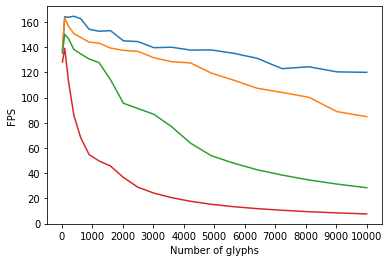
\includegraphics[width=.65\linewidth, angle=0]{figs/Esquema_Glifo/benchmark_half_texopt.png}
    \caption{FPS $\times$ quantidade de glifos renderizada. As cores azul, laranja, verde e vermelha correspondem a geometria base gerada pela $2^{a}$ $4^{a}$, $8^{a}$ e $16^{a}$ ordem de tesselação do icosaedro. Suas respectivas quantidades de vértices e triângulo são computadas nas Eq. \ref{eq::2ordem_icosphere_vertices} e \ref{eq::2ordem_icosphere_triangulos}, respectivamente.}
    \label{fig::slice_benchmark}
\end{figure}

Os resultados indicam que nosso esquema dá resultados satisfatórios para uso interativo, e mostramos que é possível renderizar milhares de glifos em taxas interativas utilizando a $4^{a}$ ordem de tesselação do icosaedro e centenas com a malha suave gerada pela $16^{a}$ ordem de tesselação.


%, no qual foi aperfeiçoado por \cite{almsick2011}. Esta abordagem possibilitou incrementos em performance em relação a \citeonline{shattuck2008}.

%\citeonline{raphael_dissertacao} propôs um esquema de renderização interativa do tensor de difusão em glifos superquádricos \cite{Kindlmann2004} utilizando polígonos. Em seu trabalho, os glifos são renderizados a taxas interativas e a sua abordagem consiste na minimização de tráfego de dados entre CPU-GPU, que consiste apenas em parâmetros que customizam e deslocam os glifos, e o uso de renderização por instâncias. Adicionalmente, este esquema está integrado ao VMTK-Neuro. Os resultados obtidos neste trabalho nos influenciou a adaptar o seu esquema para glifos HARDI.



%\subsection{\sout{Abordagem de renderização}}

%\sout{\citeonline{peeters2009} apresentou pela primeira vez um esquema de renderização para esta categoria de glifos, nos quais são aperfeiçoados por \citeonline{almsick2011} e \citeonline{hlawitschka2012}. Estes esquemas utilizam a abordagem \textit{raycasting}.}

%\sout{No VMTK-Neuro, um dos algoritmos de renderização do tensor difusão por glifos superquádricos é feita por instanciações de uma malha esférica, no qual é customizada por parâmetros particulares a cada tensor de difusão referentes a cada \textit{voxel} detectado e posicionado na cena de acordo. Este esquema de renderização desenha os glifos em tempo interativo.}

%\sout{Pela maior simplicidade e boa efetividade da renderização por instanciações de uma malha esférica, o esquema desenvolvido neste trabalho utiliza esta abordagem.}



%Dados relativos ao desempenho \sout{serão mais detalhados na dissertação de mestrado}\textcolor{blue}{estão disponíveis no link ...}.



%\sout{Medições do tempo relativo ao desempenho foram feitas para a quantidade de 197 vértices da malha esférica \sout{em um}\textcolor{blue}{num} volume de resolução 128x128x90. Para uma quantidade na faixa de 5000 glifos renderizados simultaneamente sobre uma fatia completa, obtemos tem um tempo de resposta entre 80 e 110ms. Para uma quantidade pequena de glifos na faixa das dezenas, o tempo de resposta cai para o intervalo entre 60 e 70ms. Esse tempo de resposta está nas proximidades ou é menor do que o tempo de 0,1s, que é o limite máximo para que o usuário tenha a percepção de resposta instantânea da máquina e que suas ações são a causa de que algo aconteça na tela \cite{nielsen1994}.}

%\sout{No cômputo das ODFs do \textit{QBall}, é feito o mapeamento do sinal de DWI para a ODF a partir das direções derivadas da malha esférica. O glifo para visualização é gerado diretamente de acordo a representação gráfica polar esférica em que $R(\textbf{u}) = \psi(\mathbf{u})$, onde \textbf{u} é a direção de difusão. A malha esférica utilizada para geração dos glifos em \ref{section::QBall_Glifos} está representada na figura \ref{fig::MalhaEsferico}.}

%A priori, todas as ODFs são calculadas e normalizadas para o intervalo $[0,1]$ para cada um dos \textit{voxels} do volume e referenciadas no processo de renderização.

%O formato de armazenamento dos valores ODF associados à malha consiste numa lista de valores escalares associados a cada um dos \textit{voxels}.



%\todo[inline]{Falta uma descrição melhor de como são construídos os glifos a partir de ODFs e o seu mapeamento às entidades gráficas. Isso torna difícil o entendimento da sua implementação. !!Descrito em trabalhos relacionados!}
\chapter{Renderização de funções de distribuição de orientação}
\label{chap::renderizacao_de_perfis_de_difusao}

Neste capítulo, abordamos a evolução do algoritmo de renderização de funções de distribuição de difusão feitas neste mestrado objetivando a interatividade. Apresentamos o protótipo inicial e todas as funcionalidades adicionais que implementamos durante o trabalho que culminaram no algoritmo de renderização apresentado no Capítulo \ref{chap::renderizacao_interativa_de_perfis_de_difusao}.


Na Seção \ref{sec::primeiro_prototipo}, descrevemos o estágio inicial do algoritmo, onde utilizamos a infraestrutura do ambiente de visualização multimodal para renderização dos glifos. Inicialmente, o protótipo consistiu em uma ferramenta visual para visualização de dados de ODFs em seus respectivos \textit{voxels}.

A primeira versão do algoritmo integrada ao ambiente não renderizava de forma interativa, então passamos a explorar ferramentas proporcionadas pela GPU e características da percepção visual humana para que pudéssemos otimizá-lo objetivando a interatividade. Assim, a Seção \ref{sec::renderizacao_por_instancias} discute o uso da instanciação da GPU para renderização dos glifos; a Seção \ref{sec::otimizacao_da_simetria} mostra como podemos tomar vantagem da simetria das ODFs e melhorar a performance de renderização; a Seção \ref{sec::estrutura_de_dados_para_textura_RGBA} mostra como podemos minimizar o uso de memória de textura da GPU e seu impacto em performance; e a Seção \ref{sec::adaptatividade_de_resolucao} discute como exploramos a percepção visual humana para tornar a resolução dos glifos adaptativa.

Como forma de validação que resultaram na melhor performance do algoritmo de renderização, fizemos um ambiente de renderização para testes. Em uma janela, dividimos os eixos x e y em $H$ intervalos, gerando $H^2$ células, nos quais os glifos são renderizados em cada uma delas. Cada glifo é deslocado ao centro da sua respectiva célula e escalonado para caber nela, tendo a sua geometria base fixa. A cada requisição de desenho, todos os atributos de translação que geram as ODFs e que consistem no tráfego de dados CPU-GPU são enviados à GPU, o que é demandado no ambiente de visualização multimodal, conforme mostrado no fluxograma \ref{fig::vmtk_simplified}. Variamos $H$ de cinco até cem, anotamos os dados de FPS médio e os mostramos de forma gráfica. Fizemos este experimento utilizando como geometria base, as esferas obtidas através da $2^a$, $4^a$, $8^a$ e $16^a$ ordem de tesselação do icosaedro.



O ambiente de teste é ilustrado na Fig. \ref{fig::ambiente_validacao}. Neste ambiente, as amostras que geram os glifos são computadas a priori a partir de ODFs computadas a partir de funções harmônicas esféricas, cujo o grau das funções varia de zero a três. Utilizamos esta classe de funções porque geram glifos conhecidos\footnote{A página https://chem.libretexts.org/@go/page/283935 oferece a visualização das funções harmônicas esféricas em plotagens polares esféricas.}, o que serviu de suporte para depuração. Esta classe de funções também é comumente utilizada pela comunidade HARDI e \citeonline{descoteaux2007_QBI} faz uma apresentação delas aplicada a esta área.

\begin{figure}[ht]
\centering
\captionsetup[subfloat]{farskip=5pt,nearskip=0pt}
    %!!VER SE ISSO TA CERTO
    \subfloat[H = 5. 25 glifos renderizados] {\includegraphics[width=.45\linewidth, angle=0]{figs/Renderizacao_glifos_evolucao/Ilustracao_ambiente/ambiente_5.png}
    \label{fig::ambiente_validacao_5}
    }
    \subfloat[H = 25. 625 glifos renderizados]{\includegraphics[width=.45\linewidth, angle=0]{figs/Renderizacao_glifos_evolucao/Ilustracao_ambiente/ambiente_25.png}
    \label{fig::ambiente_validacao_25}
    }
    
    \subfloat[H = 50. 2500 glifos renderizados]{\includegraphics[width=.45\linewidth, angle=0]{figs/Renderizacao_glifos_evolucao/Ilustracao_ambiente/ambiente_50.png}
    \label{fig::ambiente_validacao_50}
    }
    \subfloat[H = 100. 10000 glifos renderizados]{\includegraphics[width=.45\linewidth, angle=0]{figs/Renderizacao_glifos_evolucao/Ilustracao_ambiente/ambiente_100.png}
    \label{fig::ambiente_validacao_100}
    }
     \caption{Ambiente de avaliação do algoritmo de renderização para ODFs. As cores dos glifos referenciam a direção dos eixos de acordo com a Eq. \ref{eq::cor_glifo}.}
    %\hfill
    \label{fig::ambiente_validacao}
\end{figure}

Utilizamos dez funções harmônicas esféricas, em que, na Fig. \ref{fig::ambiente_validacao_5}, da esquerda para direita e parte superior para inferior, consistem em: $Re(Y_1^1)$,
$Re(Y_1^0)$,
$Re(Y_2^{-2})$,
$Im(Y_2^{-2})$,
$Re(Y_2^{-1})$,
$Im(Y_2^{-1})$,
$Y_2^0$,
$Y_0^0$ e
$Y_3^0$. Onde $Y_l^m$, se refere a harmônica esférica de grau $l$ e ordem $m$. Em Fig. \ref{fig::ambiente_validacao_5}, para gerar os glifos, computamos o valor absoluto das funções e fizemos a normalização min-max para o intervalo $[0, 1]$. O cômputo do valor absoluto torna estas funções simétricas em relação ao eixos coordenados, assim como as ODFs de difusão.

Nas Seções \ref{sec::renderizacao_por_instancias}, \ref{sec::otimizacao_da_simetria} e \ref{sec::estrutura_de_dados_para_textura_RGBA}, fizemos a validação da funcionalidade adicionada pela diferença em FPS de cada procedimento em relação a seção anterior de forma gráfica para cada resolução utilizada.



Na Seção \ref{sec::adaptatividade_de_resolucao}, introduzimos a adaptabilidade na resolução como uma função da máxima quantidade de \textit{pixels} contidos em um único \textit{voxel}, o que é algo intrínseco à métricas do ambiente de visualização multimodal. A validação do inserção deste tópico está nos resultados mostrados na Tabela \ref{tab::glyph_info_experiment} e a sua validação será feita através da comparação com uma versão do ambiente de visualização multimodal com glifos ODF onde a geometria base dos glifos é fixa e derivada da $8^a$ ordem do icosaedro, que está anotada na Tabela \ref{tab::glyph_info_experiment_fixed}.

As medições foram feitas em um computador Macbook Pro Retina 13', com processador Intel Core i5 Dual-Core 2.7GHz, processador gráfico integrado Intel Iris Graphics 6100 1536 MB e memória RAM de 8 GB 1867 MHz DDR3. As dimensões da janela para o ambiente de teste são $1200 \times 1200$ \textit{pixels}.



\section{Primeiro protótipo}
\label{sec::primeiro_prototipo}

No primeiro protótipo, recebendo um conjunto de índices de ODFs a serem renderizadas $D = [
\mathbf{d}_1,
\mathbf{d}_2, ..., 
\mathbf{d}_M
]$, o esquema gera três vetores para a serem enviados à GPU. O primeiro, $\mathbf{V}$, se refere ao conjunto de vértices de cada um dos glifos, $I^D$, se refere ao conjunto de índices que triangulam os vértices dos glifos e $T$ consiste nos dados de translação.

Para geração dos glifos, uma malha esférica base ($\Pi, I$) é utilizada, Onde $\Pi = [P_1, P_2, \dots, P_N]$ é o conjunto de vértices da malha, onde $P_k = [P_{xk}, P_{yk}, P_{zk}]^T$, e $I_{1\times 3\tau}$ é o conjunto de índices que triangulam $\Pi$ afim de aproximar a malha esférica, onde $\tau$ é a quantidade de triângulos da malha.

%O primeiro vetor, que consistia no conjunto de vértices de todos os glifos renderizados nos seus respectivos sistemas de coordenadas. Para isso, os vértices da malha esférica , $P_k = [P_{xk}, P_{yk}, P_{zk}]^T$ é armazenada e referenciada na CPU.

Na CPU, a matriz $\mathbf{V}_{3\times N\cdot M}$ que contém todos os vértices de todos os glifos é definida. Para isto, uma cópia dos vértices da malha esférica $\Pi$ são modulados por cada perfil de difusão dos \textit{voxels} detectados, compondo-a, como mostrado na Eq. \ref{eq::vertices_prototipo1}.

\begin{equation}
\label{eq::vertices_prototipo1}
    \mathbf{V_D} = [
    \Pi\cdot\boldsymbol{\psi}(\mathbf{d}_1)^D,
    \Pi\cdot\boldsymbol{\psi}(\mathbf{d}_2)^D,
    \Pi\cdot\boldsymbol{\psi}(\mathbf{d}_3)^D, ...,
    \Pi\cdot\boldsymbol{\psi}(\mathbf{d}_M)^D
    ]
\end{equation}

onde $\boldsymbol{\psi}(\mathbf{d}_k)_{N\times N}^D$ é a matriz diagonal, na qual cada elemento $\boldsymbol{\psi}(\mathbf{d}_k)^D[i, i]$ é dado por $\boldsymbol{\psi}(\mathbf{d}_k, \mathbf{n}_i)$, em que $\mathbf{n}_i$ é o vetor unitário com direção e sentido da normal de $P_i$.

Também na CPU, o vetor $I_{1 \times 3 \tau M}^D$ é definido e consiste na replicação de $I$ para formar as malha esférica esféricas de cada um dos objetos definidos por $\Pi\cdot\boldsymbol{\psi}(\mathbf{d}_k)^D$. Como todos os glifos são triangulados da mesma forma, $I^D$ consiste em $M$ replicações de $I$ dispostas em sequencia, na qual a k-ésima replicação consiste na adição de um fator de índice dado por $k\cdot N$. Logo $I^D$ tem a seguinte formulação:

\begin{equation}
\label{eq::index_prototipo1}
    I_D = [
    I, 
    (I +  N\mathbf{1_{3\tau}}  ),
    (I + 2N\mathbf{1_{3\tau}} ), ..., 
    (I + MN\mathbf{1_{3\tau}})
    ]
\end{equation}
onde $\mathbf{1_{3\tau}}$ é o vetor linha com todos os $3\tau$ elementos iguais a um. Observe que $I_D$ possui $3\tau M$ elementos.

Por último, $T$ consiste no conjunto de atributos de translação, que é aplicado no \textit{vertex shader} a cada vértice. Para isso, considerando as coordenadas de translação para o centro de cada \textit{voxel} $d_k$ como $V_k = [V_{kx}, V_{ky}, V_{kz}]^T$. Formulamos $T_{3 \times MN}$:

\begin{equation}
\label{eq::translation_prototipo1}
    T = [
    V_1 \cdot \mathbf{1_N},
    V_2 \cdot \mathbf{1_N},
    V_3 \cdot \mathbf{1_N}, ...,
    V_M \cdot \mathbf{1_N}
    ]
\end{equation}
onde $\mathbf{1_N}$ é o vetor linha com todos os N elementos iguais a um.

Após o envio de $\mathbf{V}$, $I^D$ e $T$ à GPU, as transformações geométricas adicionais feitas consistem na escala, para cada glifo caber em sua célula e relacionadas a multiplicação pela matriz de \textit{view-projection}. A renderização é efetuada em apenas uma chamada de desenho.

A cor é definida na GPU através da normalização para o vetor unitário do vértice do glifo no \textit{vertex shader}, e há um problema quando ODFs para cômputo direto na GPU de ODFs mapeadas em zero, no qual, neste experimento, quando isso ocorre, mapeamos em branco.

Os resultados em FPS desta abordagem estão mostrado na Fig. \ref{fig::FPS_prototipo_1}. Este protótipo é o mais próximo da abordagem \citeonline{shattuck2008}. A similaridade reside em que os vértices dos glifos são computados na CPU, mas, enquanto na nossa abordagem, as amostras já são pré-computadas, \citeonline{shattuck2008} as computa em tempo de execução a partir de funções base, implicando um custo computacional maior para renderização, que é compensado pelo menor uso de memória da CPU, pois os dados de ODF são codificados como coeficientes de funções base.



\begin{figure}[htb]
    \centering
    %\rule{6cm}{3cm}
    \includegraphics[width=.65\linewidth, angle=0]{figs/Renderizacao_glifos_evolucao/FPS_prototipo1_Geral.png}
    \caption{FPS $\times$ quantidade de glifos renderizada do primeiro protótipo. As cores azul, laranja, verde e vermelha correspondem a geometria base gerada pela $2^{a}$ $4^{a}$, $8^{a}$ e $16^{a}$ ordem de tesselação do icosaedro, respectivamente. Suas quantidades de vértices e triângulo são computadas nas Eq. \ref{eq::2ordem_icosphere_vertices} e \ref{eq::2ordem_icosphere_triangulos}, respectivamente.}
    \label{fig::FPS_prototipo_1}
\end{figure}

Esta abordagem gera um tráfego de dados excessivo entre CPU-GPU. Observe que a quantidade de dados por glifo consiste em: $N$ vértices de glifos, $3\tau$ conjunto de índices e $N$ coordenadas de translação. Codificando os vértices e coordenadas de translação em \textit{floats} e o conjunto de índices como inteiro sem sinal, onde cada um destes tipos possui quatro bytes, temos um tráfego CPU-GPU de $24N + 12\tau$ bytes por glifo. Adicionalmente, há uma redundância excessiva na quantidade de dados referentes a translação, e as operações de geração de glifos através do escalonamento dos pontos da esfera podem ser paralelizados, o que torna o potencial uso da GPU para seu cômputo uma potencial vantagem.

Observe que mesmo com o tráfego de dados excessivo, foi possível obter tempos de renderização razoáveis com as subdivisões de $2^a$ e $4^a$ ordem de tesselação.

%Poderíamos usar $M$ chamadas de desenhos, em que $I$ seria colocado na GPU como um procedimento inicial, e a cada comando de desenho, os dados de vértices dos glifo $d_k$ de ODF são computados e baixados como atributos na GPU; e de translação $V_k$ como uma variável uniforme, levando a um tráfego de $3N + 3$ floats, totalizando $12N + 12$ \textit{bytes}. Mas, o uso de instanciação da GPU, como mostrada na Seção \ref{sec::renderizacao_por_instancias}, provê um tráfego de dados menor, além do uso de apenas um comando de desenho.


\section{Instanciação}
\label{sec::renderizacao_por_instancias}

Com o objetivo de diminuir o tráfego de dados e a redundância nos dados de translação, bem como paralelizar a modulação na malha esférica base afim de obtermos os vértices do glifo, utilizamos renderização por instâncias.

A malha esférica base $(\Pi, I)$ é enviada à GPU a priori, nas quais são instanciadas $M$ vezes para os $M$ glifos a renderizar. A cada requisição de desenho, parâmetros de ODF e translação consistem no tráfego de dados CPU-GPU.

O parâmetro de translação se torna um atributo único por instância, o que pode implicar na retirada de todas as colunas repetidas de $T$, que se torna:

\begin{equation}
\label{eq::vertices_prototipo2}
    T = [
    V_1,
    V_2,
    V_3, ...,
    V_M
    ]
\end{equation}

Definimos a matriz $\mathbf{R}_{N \times M}$ que consiste em todas as amostras dos perfis de difusão do conjunto de \textit{voxels} detectados, ilustrada em Eq. \ref{eq::odf_prototipo2}.

\begin{equation}
\label{eq::odf_prototipo2}
\mathbf{R} = 
\begingroup % keep the change local
\setlength\arraycolsep{2pt}
\begin{bmatrix} 
    \psi(\mathbf{d}_{1}, \mathbf{n}_1) &
    \psi(\mathbf{d}_{2}, \mathbf{n}_1) & \cdots & 
    \psi(\mathbf{d}_{M}, \mathbf{n}_1)  \\
    
    \psi(\mathbf{d}_{1}, \mathbf{n}_2) &
    \psi(\mathbf{d}_{2}, \mathbf{n}_2) & \cdots & 
    \psi(\mathbf{d}_{M}, \mathbf{n}_2) \\ \vdots & \vdots & \vdots & \vdots  \\
    
    \psi(\mathbf{d}_{1}, \mathbf{n}_N) & 
    \psi(\mathbf{d}_{2}, \mathbf{n}_N) & \cdots & 
    \psi(\mathbf{d}_{M}, \mathbf{n}_N)
\end{bmatrix}
\endgroup
\end{equation}

Utilizamos a memória de textura para envio dos parâmetros de ODF. Para isto, enviamos $\mathbf{R}$ como uma textura 2D, de formato $RED$ e com dimensões $N\times M$. Observe que o acesso na GPU dos elementos pode ser feito a partir dos pares índice de instância e índice de vértice. Na $j$-ésima instância, onde o glifo da célula $d_j$ é processado, o \textit{lookup} na GPU é feito através da função \textit{texelFetch} das coordenadas não normalizadas $(j, Vertex\_ID)$. O acesso da ODF no processamento do vértice em sua respectiva instância é feito pela leitura do valor da componente $R$ do \textit{texel}.

Após o envio de $\mathbf{R}$ e $T$ à GPU, em adição à Seção \ref{sec::primeiro_prototipo}, o \textit{lookup} de ODFs e a modulação da malha esférica base efetuada para geração do glifo é feita no \textit{vertex shader} e somente um comando de desenho é efetuado.

Fig. \ref{fig::FPS_prototipo_2} traz de forma comparativa com o primeiro protótipo o FPS desta abordagem de renderização.

\begin{figure}[htb]
\centering
\captionsetup[subfloat]{farskip=5pt,nearskip=0pt}
    %!!VER SE ISSO TA CERTO
    \subfloat[Tesselação de $2^a$ ordem] {\includegraphics[width=.45\linewidth, angle=0] {figs/Renderizacao_glifos_evolucao/Prototipo2/prototipo_2_42.png}
    \label{fig::FPS_prototipo_2_42}
    }
    \subfloat[Tesselação de $4^a$ ordem] {\includegraphics[width=.45\linewidth, angle=0]{figs/Renderizacao_glifos_evolucao/Prototipo2/prototipo_2_162.png}
    \label{fig::FPS_prototipo_2_162}
    }
    
    \subfloat[Tesselação de $8^a$ ordem] {\includegraphics[width=.45\linewidth, angle=0]{figs/Renderizacao_glifos_evolucao/Prototipo2/prototipo_2_642.png}
    \label{fig::FPS_prototipo_2_642}
    }
    \subfloat[Tesselação de $16^a$ ordem] {\includegraphics[width=.45\linewidth, angle=0]{figs/Renderizacao_glifos_evolucao/Prototipo2/prototipo_2_2562.png}
    \label{fig::FPS_prototipo_2_2562}
    }
     \caption{FPS $\times$ Quantidade de glifos para diferentes tesselações do icosaedro. A linha preta ilustra o FPS do primeiro protótipo, enquanto a linha azul mostra o FPS da utilização da instanciação da GPU.}
    %\hfill
    \label{fig::FPS_prototipo_2}
\end{figure}


Note que o tráfego de dados CPU-GPU cai drasticamente. Para cada glifo, $N$ valores escalares de ODF são enviados a GPU, adicionalmente, conseguimos sintetizar as coordenadas de translação em um atributo único por glifo, e o conjunto de índices é apenas enviado uma vez, o que elimina o tráfego de dados relacionado a esta variável. Assim, o tráfego de dados por glifo cai para $N + 3$ floats, totalizando $4N + 12$ \textit{bytes}. Adicionalmente, a malha esférica base é modulada para gerar o glifo de forma paralela na GPU a custo de apenas uma instrução.

Note também que em todas as resoluções de glifo, o FPS mais do que dobrou em relação ao primeiro protótipo. Observe também que neste ambiente, conseguimos renderizar mais de 3000 glifos em taxas interativa \cite{nielsen1994} a partir da malha suave gerada pela $16^a$ ordem de tesselação do icosaedro. O uso de renderização por instâncias e a diminuição do tráfego de dados de amostras de ODF para apenas amostras escalares enviadas como textura foi o ponto mais crucial para interatividade.

\section{Otimização da simetria}
\label{sec::otimizacao_da_simetria}

Nesta seção, exploraremos a simetria das ODFs para que possamos diminuir o tráfego de dados de ODF discutidos na Seção \ref{sec::renderizacao_por_instancias}. Para isto, impomos a nossa primeira condição: apenas malhas esféricas com pontos simétricos em relação aos eixos são utilizadas, e os simétricos estão em sequência na memória, ou seja, em $\Pi$, N é par e $P_{2i+2} = -P_{2i+1}$, $(0 \leq i \leq \frac{N-2}{2})$, nos levando a uma estrutura de dados $\Pi = [P_1, -P_1, P_3, -P_3, \dots, P_{N-3}, -P_{N-3}, P_{N-1}, -P_{N-1}]$.

Neste contexto, na formação do glifo ODF do \textit{voxel} $\mathbf{r}$, $\psi(\mathbf{r}, \mathbf{n}_{2i+1})$ escalona os pontos $P_{2i+1}$ e $P_{2i+2}$ da esfera. Logo, reestruturamos $\mathbf{R}$ para que se torne $\mathbf{R}_{\frac{N}{2}\times M}$, nos quais receba apenas as ODFs de sub-índice ímpar, conforme mostrado na Eq. \ref{eq::odf_prototipo3}.

\begin{equation}
\label{eq::odf_prototipo3}
\mathbf{R} = 
\begingroup % keep the change local
\setlength\arraycolsep{2pt}
\begin{bmatrix} 
    \psi(\mathbf{d}_{1}, \mathbf{n}_1) &
    \psi(\mathbf{d}_{2}, \mathbf{n}_1) & \cdots & 
    \psi(\mathbf{d}_{M}, \mathbf{n}_1)  \\
    
    \psi(\mathbf{d}_{1}, \mathbf{n}_3) &
    \psi(\mathbf{d}_{2}, \mathbf{n}_3) & \cdots & 
    \psi(\mathbf{d}_{M}, \mathbf{n}_3) \\ \vdots & \vdots & \vdots & \vdots  \\
    
    \psi(\mathbf{d}_{1}, \mathbf{n}_{N-1}) & 
    \psi(\mathbf{d}_{2}, \mathbf{n}_{N-1}) & \cdots & 
    \psi(\mathbf{d}_{M}, \mathbf{n}_{N-1})
\end{bmatrix}
\endgroup
\end{equation}

Assim como na Seção \ref{sec::renderizacao_por_instancias}, enviamos $\mathbf{R}$ como uma textura 2D, de formato $RED$, com dimensões $\frac{N}{2}\times M$. Observe que o acesso na GPU dos elementos é modificado em função do Vertex\_ID. Na $j$-ésima instância, onde o glifo do \textit{voxel} $d_j$ é processado, o \textit{lookup} na GPU é feito através da função \textit{texelFetch} das coordenadas não normalizadas $\lfloor (j, Vertex\_ID/2)\rfloor$. O acesso da ODF no processamento do vértice em sua respectiva instância é feito pela leitura do valor da componente $R$ do \textit{texel}.\footnote{A função em OpenGL para \textit{lookup} em função dos índices de instância e vértice é dada por texelFetch($\mathbf{R}$,ivec2((gl\_VertexID)/2, gl\_InstanceID), 0).r}.  Conforme ilustrado na Fig. \ref{fig::texelfetch_prototipo3}.

\begin{figure}[htb]
%\subfigcapskip = -5pt
    \centering
    \includegraphics[width=.35\linewidth, angle=0]{figs/Renderizacao_glifos_evolucao/texellookup_RED.png}
    \caption{Ilustração do acesso nas componentes RGBA em \textit{texel} na textura \textbf{R} no índice $K$ e $j$. O \textit{texel} é acessado pelas threads que processam os vertices de índices 2K e 2K+1 em uma instância $j$. Os blocos de contorno vermelho, azul, verde e cinza ilustram as componentes R,G,B e A do \textit{texel}, respectivamente. Observe que as componentes G, B e A são inicializadas com valores \textit{default}.}
    \label{fig::texelfetch_prototipo3}
   %\hspace{1pt}
\end{figure}


Fig. \ref{fig::FPS_prototipo_3} traz de forma comparativa com o FPS da Seção \ref{sec::renderizacao_por_instancias} o ganho em FPS desta abordagem de renderização.

\begin{figure}[H]
\centering
\captionsetup[subfloat]{farskip=5pt,nearskip=0pt}
    %!!VER SE ISSO TA CERTO
    \subfloat[Tesselação de $2^a$ ordem] {\includegraphics[width=.45\linewidth, angle=0]{figs/Renderizacao_glifos_evolucao/Prototipo3/prototipo_3_42.png}
    \label{fig::FPS_prototipo_3_42}
    }
    \subfloat[Tesselação de $4^a$ ordem] {\includegraphics[width=.45\linewidth, angle=0]{figs/Renderizacao_glifos_evolucao/Prototipo3/prototipo_3_162.png}
    \label{fig::FPS_prototipo_3_162}
    }
    
    \subfloat[Tesselação de $8^a$ ordem] {\includegraphics[width=.45\linewidth, angle=0]{figs/Renderizacao_glifos_evolucao/Prototipo3/prototipo_3_642.png}
    \label{fig::FPS_prototipo_3_642}
    }
    \subfloat[Tesselação de $16^a$ ordem] {\includegraphics[width=.45\linewidth, angle=0]{figs/Renderizacao_glifos_evolucao/Prototipo3/prototipo_3_2562.png}
    \label{fig::FPS_prototipo_3_2562}
    }
     \caption{FPS $\times$ Quantidade de glifos para diferentes tesselações do icosaedro. A linha pontilhada azul ilustra o FPS do segundo protótipo, enquanto a linha vermelha mostra o FPS quando tomamos vantagem da simetria das ODF.}
    %\hfill
    \label{fig::FPS_prototipo_3}
\end{figure}



Observe que esta otimização faz o tráfego de dados CPU-GPU ser reduzido de $N + 3$ para $N/2 + 3$ \textit{floats}, totalizando $2N + 12$ bytes. Em termos de performance, observe em Fig. \ref{fig::FPS_prototipo_3_642} e \ref{fig::FPS_prototipo_3_2562}, aproximadamente 4900 e 1225 glifos puderam ser renderizados a 60 FPS para $8^a$ e $16^a$ ordem de tesselação, enquanto na abordagem em que não tomamos vantagem da simetria, 3600 e 900 puderam ser gerados para este FPS.

Por outro lado, observe que os maiores ganhos de performance ocorrem na faixa que compreendem 600 a 1600 glifos para $16^a$ ordem de tesselação e 2400 até 5000 glifos para para $8^a$, no qual, nesta região, há um ganho em FPS acima de 20\%.

Note que as componentes B, G e A do \textit{texel} são alocadas, setadas para valores padrão e não são utilizadas\footnote{Informações sobre a alocação de memória em uma textura de formato RED pode ser encontrada em https://www.khronos.org/registry/OpenGL-Refpages/gl4/html/glTexImage2D.xhtml}. Adicionalmente, as componentes R, G, B e A na memória de textura em cada \textit{texel} estão em sequencia na GPU e nesta abordagem, as amostras de ODF estão espaçadas em 3 \textit{floats}. Neste leiaute de memória, no qual os coeficientes de ODF não estão em sequência, não utilizamos o cache da GPU de forma ótima.



\section{Estrutura de dados para textura RGBA}
\label{sec::estrutura_de_dados_para_textura_RGBA}

Para evitar o desperdício de memória e mau uso do cache da GPU, enviamos $\mathbf{R}$ como uma textura de formato RGBA, de tamanho $\lceil \frac{N/2}{4}\rceil \times M$ em que agrupamos os valores escalares da $j$-ésima coluna em sequência de quatro em quatro. Se $N/2$ não é divisível por quatro, é necessária a inserção de linhas com valores \textit{dummy} em $\mathbf{R}$ afim de completar a divisibilidade por quatro, para que cada coluna da matriz possa ser acessada via índice de instância.

Assim, em cada \textit{texel} há quatro amostras de ODF que modulam 8 pontos da malha esférica. Desta forma, cada \textit{texel} é acessado por 8 \textit{threads}. No Capítulo \ref{chap::renderizacao_interativa_de_perfis_de_difusao}, a Fig. \ref{fig::texelfetch} ilustra a forma que o \textit{lookup} é feito. O argumento da função \textit{texelFetch} para a $j$-ésima instância se torna as coordenadas não-normalizadas $(j, \lfloor \frac{Vertex\_ID}{8} \rfloor)$ e o acesso do ponto processado a seu respectivo valor de ODF, considerando que as componentes R, G, B e A são mapeados nos índices 0, 1, 2 e 3 nos \textit{texels} é mapeado por $\lfloor Vertex\_ID \mod{8}/2 \rfloor$.

Fig. \ref{fig::FPS_prototipo_4} traz de forma comparativa o FPS gerado por esta nova organização de $\mathbf{R}$ no envio como textura em comparação à Seção \ref{sec::otimizacao_da_simetria}.

\begin{figure}[ht]
\centering
\captionsetup[subfloat]{farskip=5pt,nearskip=0pt}
    %!!VER SE ISSO TA CERTO
    \subfloat[Tesselação de $2^a$ ordem] {\includegraphics[width=.45\linewidth, angle=0]{figs/Renderizacao_glifos_evolucao/Prototipo4/prototipo_4_42.png}
    \label{fig::FPS_prototipo_4_42}
    }
    \subfloat[Tesselação de $4^a$ ordem] {\includegraphics[width=.45\linewidth, angle=0]{figs/Renderizacao_glifos_evolucao/Prototipo4/prototipo_4_162.png}
    \label{fig::FPS_prototipo_4_162}
    }
    
    \subfloat[Tesselação de $8^a$ ordem] {\includegraphics[width=.45\linewidth, angle=0]{figs/Renderizacao_glifos_evolucao/Prototipo4/prototipo_4_642.png}
    \label{fig::FPS_prototipo_4_642}
    }
    \subfloat[Tesselação de $16^a$ ordem] {\includegraphics[width=.45\linewidth, angle=0]{figs/Renderizacao_glifos_evolucao/Prototipo4/prototipo_4_2562.png}
    \label{fig::FPS_prototipo_4_2562}
    }
     \caption{FPS $\times$ Quantidade de glifos para diferentes tesselações do icosaedro. A linha pontilhada vermelha ilustra o FPS do terceiro protótipo, enquanto a linha magenta mostra o FPS do uso das componentes RGBA dos \textit{texels} da memória de textura.}
    %\hfill
    \label{fig::FPS_prototipo_4}
\end{figure}


Observe que este procedimento faz o tráfego de dados CPU-GPU ser sutilmente aumentado para $N/2 + 3 + (-N/2 \mod{4})$, mas a quantidade de memória alocada para $\mathbf{R}$ na GPU cai para aproximadamente um quarto em comparação à abordagem anterior.

Observe que há um aumento sutil em FPS quando milhares de glifos são renderizados a partir das malhas da $8^a$ e $16^a$ ordem de subdivisão. Isso ocorre devido a maior alocação de dados de ODF no cache da GPU devido a este procedimento.


\section{Adaptatividade de resolução}
\label{sec::adaptatividade_de_resolucao}

Aplicamos todos os conceitos apresentados até a versão do algoritmo de renderização de ODFs, apresentada na Seção \ref{sec::estrutura_de_dados_para_textura_RGBA}, integramos ao ambiente de visualização multimodal e fizemos as medições de performance conforme descrita em \ref{ssec::performance}, onde utilizamos a tesselação de $8^a$ ordem do icosaedro de forma fixa, cujos resultados estão apresentados na Tabela \ref{tab::glyph_info_experiment_fixed}.

No experimento, ao compararmos a integração do algoritmo com a estrutura apresentada no Capítulo \ref{chap::renderizacao_interativa_de_perfis_de_difusao}, o algoritmo integrado ao ambiente multimodal recebe apenas o conjunto de \textit{voxels} detectados como entrada. O cômputo de $max_p$ feito na GPU e o algoritmo de escolha da geometria base foram desativados para fins de teste.

Usamos o mesmo volume e métodos descrito na seção \ref{sec::experimentos} do Capítulo \ref{chap::renderizacao_interativa_de_perfis_de_difusao} para gerar os resultados.

\begin{table}[]
\centering
\begin{tabular}{|cccc|}
\hline
\textbf{FPS} & \textbf{Fator de escala} & \textbf{\# glifos} & \textbf{\begin{tabular}[c]{@{}c@{}}Ordem de \\ tesselação\end{tabular}} \\ \hline
34.29 & 86.50 & 12     & 8 \\
35.23 & 58.15 & 20     & 8 \\
35.43 & 38.76 & 42     & 8 \\
35.83 & 25.84 & 90     & 8 \\
32.78 & 17.23 & 182    & 8 \\
35.70 & 11.49 & 380    & 8 \\
32.96 & 7.66  & 870    & 8 \\
28.53 & 5.10  & 1892   & 8 \\
23.17 & 3.40  & 4160   & 8 \\
14.58 & 2.27  & 9166   & 8 \\
 7.96 & 1.51  & 13205  & 8 \\
\hline
\end{tabular}
\caption{Esquema de renderização multimodal com glifos ODF renderizados em uma imagem $850\times 850$ com a geometria base fixa. A última linha da tabela descreve a geração da imagem na Fig. \ref{fig::multimodal_highres} no apêndice.}
\label{tab::glyph_info_experiment_fixed}
\end{table}

Observe que não conseguimos renderizar os glifos em taxas interativas quando há muitos deles sendo renderizados e, por isso, resolvemos tornar a geometria base adaptativa. Assim, dividimos o problema em em duas partes: (1) como podemos alternar geometrias base para sub-malhas da malha esférica base na qual as ODFs são amostradas em tempo de execução; e (2) como podemos diminuir o tráfego de dados para que apenas os dados das sub-malhas sejam enviados à GPU.

Com este objetivo, propomos a segunda condição: a malha esférica base $(\Pi, I)$ tem $k$ sub-malhas onde cada sub-malha é denotada por $(\Pi_i, I_i)$,  $(0 \leq i < k)$, adicionalmente, o número de pontos das sub-malhas é crescente de acordo com os sub-índices, i.e. se $(0 \leq i < j < k)$, implica $|\Pi_j| > |\Pi_i|$. Os primeiros $|\Pi_i|$ elementos na estrutura de dados de $\Pi$ corresponde aos elementos de $\Pi_i$. Note que esta condição também implica que, para $i$, $j$ tais $0 \leq i < j < k$, $\Pi_i$ é subconjunto de $\Pi_j$.

Aplicadas estas condições, resolvemos a alternância de malhas esféricas, fazendo com que, no processo de inicialização do esquema de renderização, a malha $(\Pi, I)$ e todos os conjunto de índices das sub-malhas são carregados na GPU. Resolvemos o problema de tráfego de dados no cômputo das amostras de ODF, no qual as amostras que são projetadas na sub-malha esférica de mais baixa resolução são colocadas na parte inicial de $\boldsymbol{\psi(\mathbf{r})}$, as amostras que são projetadas na malha esférica de segunda mais baixa resolução, envolve as amostras da primeira e as suas próprias amostras em $\boldsymbol{\psi(\mathbf{r})}$, e assim por diante.

Sugerimos tesselações do icosaedro de ordem potência de dois para este fim. A forma que escolhemos para fazer a escolha entre uma destas é baseado na relação empírica e heurística de \citeonline{voltoline2021}, que estabelece uma quantidade mínima de triângulos para manutenção de uma boa qualidade visual dos glifos, dado a sua ocupância em \textit{pixels}, que está formulada nos tópicos \ref{sssec::formulação_da_geometria_e_estruturação_de_dados}, \ref{sssec::escolha_automatica_da_geometria_base} e \ref{sssec::dados_de_odf}.

Na Seção \ref{sec::qualidade_visual_longe} do apêndice, apresentamos duas imagens com muitos glifos com as geometria base derivadas da $2^a$ e $8^a$ ordem de tesselação integradas ao ambiente de visualização multimodal, em que estão mapeadas nas Fig. \ref{fig::qualidade_visual_longe_lowres} e \ref{fig::qualidade_visual_longe_highres}, respectivamente. Nelas, podemos observar que não há diferença visual perceptível, o que nos leva a crer que não há contrapartida em qualidade visual dos glifos para adaptabilidade da geometria base.

Na Tabela \ref{tab::glyph_info_experiment} do capítulo \ref{chap::renderizacao_interativa_de_perfis_de_difusao} consta o experimento feito com a malha esférica adaptativa, e ao comparamos os resultados entre ambas, podemos concluir que conseguimos obter aproximadamente 10 FPS a mais quando 13205 glifos são renderizados e 8,5 FPS quando pouco mais de 9000 glifos são renderizados, e que conseguimos uma solução satisfatória que resolve o problema da interatividade da visualização quando uma grande quantidade de glifos é renderizada.

Acerca da diminuição do FPS mostrada na tabela \ref{tab::glyph_info_experiment}. Vimos que nos gráficos da Fig. \ref{fig::FPS_prototipo_4_42} e \ref{fig::FPS_prototipo_4_162}, os FPS se mantém muito altos quando a quantidade de glifos chega próximo a 10000 para o uso de uma malha de baixa resolução. Isso mostra que o gargalo que diminui a performance do algoritmo, mesmo com a malha adaptativa está relacionada ao tráfego de dados GPU-CPU com as coordenadas dos \textit{voxels} detectados. Nesta abordagem de renderização, não podemos compensar este gargalo pois a alta dimensionalidade das ODFs, que são armazenadas como amostras, tornam inviável o seu armazenamento completo na GPU e isso nos impede de usar a estratégia de \citeonline{voltoline2021}, no qual os parâmetros que customizam as superquádricas são armazenados na GPU.


\chapter{Conclusão}
\label{chap::conclusao}


Neste trabalho abordamos a renderização de funções de distribuição de orientação de métodos de alta ordem para DWI integrado a um ambiente de visualização multimodal que envolve DWI co-registrado a volumes escalares de outras modalidades \cite{VMTKNeuro}. Para alcançar este objetivo, implementamos o cômputo do método de alta ordem Amostragem Generalizada no Espaço-Q e a visualização das ODFs estimadas, aproveitando a infraestrutura e funcionalidades implementadas de co-registro entre dois volumes \cite{ting2014} e a infraestrutura para renderização multimodal para DTI e glifos superquádricos \cite{voltoline2021}.

Para estimação de ODFs de difusão, implementamos o cômputo do método de imageamento amostragem generalizada no espaço-Q de acordo com o sugerido por \citeonline{yeh2010}. Derivamos o método até chegarmos em uma formulação que relaciona o sinal e o perfil de difusão em uma ODF através de uma multiplicação matricial. Armazenamos as ODFs em amostras e exploramos sua simetria para armazenarmos ODFs de direções simétricas em um somente um valor.

Afim de prover um ambiente que se propõe a ser utilizado para avaliação de ODFs, desenvolvemos um algoritmo de renderização de ODFs em glifos, nos quais são posicionados em seus respectivos \textit{voxels} na renderização multimodal. Nos baseamos no algoritmo de renderização multimodal para volumes de ressonância magnética DWI e T1 co-registrados com glifos superquádricos proposto por \citeonline{voltoline2021} e exploramos a simetria de ODFs e a percepção visual humana para renderizar os glifos em tempo interativo.

Levando estes pontos em consideração, propomos uma forma de estruturar dados de amostras de ODF armazenadas na CPU. Adicionalmente, propomos o cômputo da resolução da malha, como os dados são enviados e acessados na GPU para gerar cada um dos glifos e como utilizamos a renderização por instanciação para gerar múltiplos glifos com um comando de desenho.

Nos experimentos que fizemos, atestamos que o algoritmo integrado ao ambiente de visualização multimodal renderiza quadros a uma taxa interativa e também mostramos que, através deles, é possível inferir acerca de cruzamentos de fibras.

\section{Futuros Trabalhos}

Para futuros trabalhos, podemos pesquisar o cômputo da distribuição local de fibras subjacentes às ODFs, bem como pesquisar e desenvolver uma abordagem de tractografia para gerar tratos do cérebro baseados na distribuição local, como mostrado no fluxograma da Fig. \ref{fig::flowchart_vmtk_hardi}. Podemos explorar o algoritmo de \citeonline{Chamberland2016}, que propôs um algoritmo onde as fibras são reconstruídas em tempo interativo a partir de distribuição local de fibras subjacentes pré-computadas e que entram de acordo com a visualização interativa proposta no VMTK-Neuro. Ressaltamos que métodos de tractografia baseadas em ODFs é um problema em aberto e alguns dos desafios da área podem ser encontrados em \citeonline{SCHILLING2019194}.

Por questões de otimização no uso de memória, que é muito demandada por ODFs de métodos de alta ordem, destacamos que é importante que haja uma forma de segmentar o cérebro para o volume de difusão, para que as amostras de ODF não sejam computadas e alocadas na memória para \textit{voxels} que não estão contidos no cérebro.

Na renderização multimodal para glifos ODF, podemos investigar a adaptação do algoritmo de renderização de glifos para ODFs que estejam representadas como funções base harmônicas esféricas, que são frequentemente utilizadas na comunidade HARDI \cite{descoteaux2007_QBI, Tournier2004DirectEO}.


%bem como desenvolver aplicações de visualização associadas. Adaptando muito do que já fora desenvolvido para o DTI, as aplicações desenvolvidas para o método consistem na estimação de ODFs via transformada de Funk-Radon, visualização em tempo interativo de ODFs em glifos e o desenvolvimento de um algoritmo de tractografia associado.

%Objetivando prover um ambiente que permite a avaliação de ODFs, aproveitando as funcionalidades presentes no VMTK-Neuro para exploração de DWIs e MRI anatômicos, foi desenvolvido um esquema de renderização em tempo interativo que mapeia as ODFs em suas representações gráficas polares esféricas.

%Com o objetivo de melhorar e tractografia baseada em DTI, foi implementado um protótipo de algoritmo de tractografia baseado em um conjunto de direções de métodos HARDI. !!(No trato corticoespinhal, no qual o DTI não consegue resolver).
%Adicionalmente, a tractografia gera resultados em tempo interativo para o usuário, permitindo-o explorar livremente para diferentes parâmetros.

%\section{Futuros trabalhos}

%Na renderização de glifos, pode-se implementar o cômputo de vetores normais para serem usados na iluminação das superfícies, o que é algo comum na apresentação por glifos. Adicionalmente, podemos implementar as representações polares esféricas sugerida por \citeonline{hlawitschka2012} e/ou \citeonline{almsick2011} para fins de comparação de performance com a nossa abordagem.

%Em tractografia, o próximo passo é a implementação do afiamento de ODFs, o que melhora extração de direções plausíveis de direções a serem usadas no \textit{tracking} de fibras \cite{fillard2011, SCHILLING2019194}.
\pagebreak
 \chapter{Apêndice}
 \section{Qualidade visual dos glifos a uma visão distante}
 \label{sec::qualidade_visual_longe}


% \section{Imagens de ODFs mapeadas em glifos renderizadas no VMTK-Neuro}

% \label{section::QBall_Glifos}

 \begin{figure}[H]
 %\subfigcapskip = -5pt
     \centering
     \includegraphics[width=1.0\linewidth, angle=0]{figs/Renderizacao_glifos_evolucao/Adaptividade-multimodal/Fatia_42.png}
      \caption{13205 glifos renderizados sobre um volume \textit{ray-casted}. A geometria base utilizada é proveniente da tesselação de $2^a$ ordem do icosaedro.}
       \label{fig::qualidade_visual_longe_lowres}
  %   \hspace{1pt}
 \end{figure}
 
  \begin{figure}[H]
 %\subfigcapskip = -5pt
     \centering
     \includegraphics[width=1.0\linewidth, angle=0]{figs/Renderizacao_glifos_evolucao/Adaptividade-multimodal/Fatia_642.png}
      \caption{13205 glifos renderizados sobre um volume \textit{ray-casted}. A geometria base utilizada é proveniente da tesselação de $8^a$ ordem do icosaedro.}
       \label{fig::qualidade_visual_longe_highres}
  %   \hspace{1pt}
 \end{figure}

% \begin{figure}[H]
% \label{fig::QBall_glifos_sagital}
% %\subfigcapskip = -5pt
%     \centering

%     \includegraphics[width=.7\linewidth, angle=0]{figs/Exemplos_QBall_visualizacao/Sagital.png}
%     \caption{Projeção Sagital.}
%  %   \hspace{1pt}
% \end{figure}

% \begin{figure}[H]
% \label{fig::QBall_glifos_coronal}
% %\subfigcapskip = -5pt
%     \centering

%     \includegraphics[width=0.7\linewidth, angle=0]{figs/Exemplos_QBall_visualizacao/Coronal.png}
%     \caption{Projeção Coronal.}
%  %   \hspace{1pt}
% \end{figure}

% \begin{figure}[H]
% \label{fig::QBall_glifos_Coronal_CC_CS}
% %\subfigcapskip = -5pt
%     \centering
%     \includegraphics[width=.7\linewidth, angle=0]{figs/Exemplos_QBall_visualizacao/Coronal_Cruzamento_MapaFA.png}
%     \caption{Projeção Coronal - Região de cruzamento de fibras. Glifos renderizado sobre mapa FA codificado por cores do DTI.}
%  %   \hspace{1pt}
% \end{figure}

% \begin{figure}[H]
% \label{fig::QBall_glifos_azul}
% %\subfigcapskip = -5pt
%     \centering

%     \includegraphics[width=.4\linewidth, angle=0]{figs/Exemplos_QBall_visualizacao/Glifo_Azul.png}
%     \caption{Glifo referente a um voxel com direção de difusão predominantemente ascendente.}
%  %   \hspace{1pt}
% \end{figure}

\pagebreak


% \section{\textit{Overplus} e problemas com o mapeamento do sinal de difusão em ODFs}
% \label{ssec::problema_overplus}

% Após um estudo que visou comparar ODFs geradas a partir de diferentes esquemas de amostragem de gradientes de ponderação de difusão, concluímos que a falta de uniformidade do conjunto de gradientes do \textit{Overplus} no domínio esférico compromete a interpolação de sinais de difusão no processo de cômputo do \textit{Q-Ball}. A figura \ref{fig::shell_Overplus_VS_ISMRM} mostra a distribuição no \textit{shell}\footnote{\textit{Shell} é um consiste em um conjunto definido em uma esfera.} das direções dos gradientes do \textit{Overplus}, em adição ao utilizado no volume ISMRM 2015.

% \begin{figure}[ht]
% \centering
% \captionsetup[subfloat]{farskip=5pt,nearskip=0pt}
%     %!!VER SE ISSO TA CERTO
%     \subfloat[\textit{Overplus}.] {\includegraphics[width=.4\linewidth, angle=0]{figs/Overplus_VS_ISMRM/shell_overplus.png}}    
%     \hfill
%     \subfloat[Esquema utilizado no ISMRM.]{\includegraphics[width=.4\linewidth, angle=0]{figs/Overplus_VS_ISMRM/shell_ismrm.png}}
%      \caption{Domínio esférico com pontos de amostragem referentes a direção de gradientes de difusão. Vermelho: direções de amostragem. Azul: sentido oposto da direção de amostragem.}
%     %\hfill
%     \label{fig::shell_Overplus_VS_ISMRM}
% \end{figure}


% Um bom conjunto de gradientes de codificação de difusão vinculada a um DWI não tem uma preferência direcional, as amostras no domínio esférico possuem uma boa invariância à orientação das estruturas do tecido ou coordenadas da máquina e a separação angular entre um par de pontos mais próximos é máxima e constante para todos os elementos \cite{cheng2018}. Um conjunto que segue essas propriedades estão distribuídos uniformemente sobre o \textit{shell}.

% Há uma certa concordância na literatura de que uma uniformidade no domínio esférico em aquisições \textit{single shell}\footnote{Denomina-se aquisição \textit{single shell} como volumes de ressonância de difusão escaneados com apenas um valor b, além do b0.} é importante para uma boa reconstrução de ODFs. \citeonline{yeh2010} mencionam a importância da uniformidade além de propor uma métrica para aferir o seu grau. \citeonline{cheng2018} discorrem sobre formulações de esquemas de amostragem de gradientes de forma uniforme e mencionam as suas vantagens.

% Como parte do processo de investigação dos resultados não esperados de ODFs gerados a partir dos volumes adquiridos através do protocolo \textit{Overplus}, foram escaneados para um mesmo indivíduo um volume com o conjunto de direções da competição ISMRM, o padrão, e um usando o protocolo \textit{Overplus} da Philips, em que todos possuem a mesma resolução angular de 32 direções. A análise feita consistiu na inspeção da forma dos glifos na região do corpo caloso que contém uma forte componente na direção mediolateral. A localização desta região se dá através do mapa FA codificado por cor gerado pelo DTI, em que não foi constatado nenhum problema nestes esquemas de aquisição.


% Nesta inspeção, foi possível gerar glifos das ODFs razoáveis para o esquema de amostragem do ISMRM (Figura \ref{fig::Overplus_VS_ISMRM_b}), o que não aconteceu com o \textit{Overplus}, em que as ODFs ficaram totalmente descaracterizadas em comparação com os códigos de cores, conforme mostrado na Figura \ref{fig::Overplus_VS_ISMRM_a}.

% \begin{figure}[ht]
% \centering
% \captionsetup[subfloat]{farskip=5pt,nearskip=0pt}
    
%     \subfloat[\textit{Overplus}] {\label{fig::Overplus_VS_ISMRM_a} \includegraphics[width=.45\linewidth, angle=0, ]{figs/Overplus_VS_ISMRM/Overplus.png}}
%     \hfill
%     \subfloat[Esquema da competição ISMRM]{\label{fig::Overplus_VS_ISMRM_b} \includegraphics[width=.47\linewidth, angle=0]{figs/Overplus_VS_ISMRM/ISMRM.png}}
%     %\hfill
%     \caption{Glifos do Corpo Caloso - Mediolateral. Glifos de ODF sobre mapa FA codificado por cor do DTI.} %!!VER SE ISSO TA CERTO
%     \label{fig::Overplus_VS_ISMRM}
% \end{figure}
\pagebreak


%\bibliographystyle{}
\bibliography{references.bib}

% ----------------------------------------------------------
% Glossário
% ----------------------------------------------------------
%
% Consulte o manual da classe abntex2 para orientações sobre o glossário.
%
%\glossary

% ----------------------------------------------------------
% Apêndices
% ----------------------------------------------------------

% ---
% Inicia os apêndices
% ---
%\begin{apendicesenv}
%\end{apendicesenv}
% ---


% ----------------------------------------------------------
% Anexos
% ----------------------------------------------------------

% ---
% Inicia os anexos
% ---
\begin{anexosenv}
\end{anexosenv}

%---------------------------------------------------------------------
% INDICE REMISSIVO
%---------------------------------------------------------------------
%\phantompart
\printindex
%---------------------------------------------------------------------

\end{document}


